\documentclass[11pt,a4paper]{article}

\usepackage[utf8]{inputenc}
\usepackage[T1]{fontenc}
\usepackage{lmodern}
\usepackage[a4paper,margin=0.82in]{geometry}
\usepackage{amsmath,amssymb,amsthm}
\usepackage{booktabs}
\usepackage{longtable}
\usepackage{array}
\usepackage{graphicx}
\usepackage{xcolor}
\usepackage{hyperref}

\hypersetup{
    colorlinks=true,
    linkcolor=blue!70!black,
    citecolor=blue!70!black,
    urlcolor=blue!70!black,
    pdftitle={Black Holes, the Big Bang, and Present Cosmic Expansion as Dual Painleve-Gullstrand Regimes of the Discrete K4 Temporal Substrate},
    pdfauthor={Jolcsak, A. (Tau Core Research Collaboration)}
}

\setlength{\emergencystretch}{2em}
\newcolumntype{L}[1]{>{\raggedright\arraybackslash}p{#1}}
\newcolumntype{C}[1]{>{\centering\arraybackslash}p{#1}}
\newcolumntype{R}[1]{>{\raggedleft\arraybackslash}p{#1}}

\newtheorem{theorem}{Theorem}[section]
\newtheorem{proposition}[theorem]{Proposition}
\newtheorem{corollary}[theorem]{Corollary}
\theoremstyle{remark}
\newtheorem{remark}[theorem]{Remark}

\title{\textbf{Black Holes, the Big Bang, and Present Cosmic Expansion as Dual Painlev\'e--Gullstrand Regimes of the Discrete $K_4$ Temporal Substrate:\\
Non-Singular Anatomy, Horizon Thermodynamics, and Multi-Probe Validation ($k = 0$)}}

\author{Jolcsak, A.\\
\small\textit{Tau Core Research Collaboration} (\texttt{tau-core-black-hole-cosmology-duality-paper21})}

\date{14 November 2026}

\begin{document}
\maketitle

\begin{abstract}
\noindent
General Relativity (GR) coupled to the $\Lambda$ Cold Dark Matter ($\Lambda\mathrm{CDM}$) model treats six foundational anomalies of gravitational physics---(i) central black hole curvature singularities ($r \to 0$) and inner Cauchy-horizon mass inflation, (ii) the initial Big Bang singularity ($a \to 0$), (iii) the $10^{122}$-order-of-magnitude quantum-vacuum cosmological-constant catastrophe, (iv) Penrose's past-Weyl horizon-entropy paradox, (v) galactic and cluster ``dark matter'' kinematics and lensing, and (vi) late-time cosmic ``dark energy'' acceleration---as logically disconnected puzzles requiring independent auxiliary postulates. Here we prove analytically (verified symbolically via \texttt{SymPy}) and test across multi-messenger strong-field and cosmological observations that under the source-frozen \textbf{Tau Core Three-Pillar Canonical Synthesis ($k = 0$ free tuned parameters)}, black hole interiors and cosmic expansion emerge as exact sign-reversed regimes ($\sigma_{\mathrm{flow}} = -1$ versus $\sigma_{\mathrm{flow}} = +1$) of a single Painlev\'e--Gullstrand (PG) acoustic clock fluid governed by the discrete $K_4$ pregeometric simplex.

Specifically, we establish five exact theorems (\texttt{Theorems D1--D5}):
\textbf{(D1)} A unified PG metric with flat spatial hypersurfaces, radial null speeds $\dot{r}_\pm = c(\pm 1 + \sigma_{\mathrm{flow}}\beta)$, occupied-block seed light-cone shift $g_{0r}(1/4) = -\sqrt{5}/8 \approx -0.27951$, and connection-free Cartan--Kodama exterior 2-form holonomy $\mathrm{d}K$ yields $\kappa_{\mathrm{BH}} = c^2/(2r_s)$ for stationary black holes ($\sigma_{\mathrm{flow}} = -1$) and $|\kappa_{\mathrm{KH}}(z)| = \frac{1}{2}cH(z)|1 - q(z)| = cH(z)|1 - \frac{3}{4}\Omega_m(z)|$ for the expanding cosmos ($\sigma_{\mathrm{flow}} = +1$).
\textbf{(D2)} In spatially flat matter plus $\Lambda$-asymptote FLRW cosmology, the onset of cosmic acceleration $q(z_{\mathrm{acc}}) = 0$ ($\ddot{a} = 0$) and the minimum of the galactic Kodama--Hayward acceleration trajectory $\mathrm{d}a_0^{\mathrm{KH}}/\mathrm{d}z = 0$ occur at the \emph{exact same cosmic epoch} $\Omega_m(z) = 2/3$, giving $z_{\mathrm{acc}} \equiv z_{\mathrm{dip}} = (2\Omega_{\Lambda,0}/\Omega_{m,0})^{1/3} - 1 = 0.63155650$ ($a_0^{\mathrm{KH}}(z_{\mathrm{dip}})/a_0^{\mathrm{KH}}(0) = 0.93855026$).
\textbf{(D3--D4)} Inside $r < r_s$, gravitational collapse traverses four regular concentric zones: supersonic PG inflow with traceless $+2:-1:-1$ \texttt{CHDF} Weyl stretching (\textbf{Zone I}), short-range \texttt{COCA-H1} Yukawa subtraction cancelling the $1/r^2$ singularity to a finite core self-force $+\frac{1}{2}GM m_{\mathrm{COCA}}^2$ alongside chiral 48-Weyl deconfinement (\textbf{Zone II}), 15-channel \texttt{CHDF} UV trace cancellation $\mathrm{Tr}(T_{\mathrm{def}}^{(15)}) = 0$ arresting Cauchy-horizon mass inflation at $x_- \approx 0.0323$ with $\pi_2(S^2) = \mathbb{Z}$ spin-texture angular-momentum storage (\textbf{Zone III}), and an incompressible de Sitter $K_4$ Seed Core enforced by Clifford-projector superselection $\Pi^2 = \Pi \implies r_{\mathrm{seed}} = 1/4$, $\dot{r} \equiv 0$ with $f_{\mathrm{eff}}(0) = +1$, $w(0) = -1$, and Planckian curvature ceiling $\mathcal{K}_{\max}\ell_P^4 = \frac{1}{24\pi^2} \approx 4.22 \times 10^{-3}$ (\textbf{Zone IV}). Under $\sigma_{\mathrm{flow}} = +1$, cosmic genesis undergoes a smooth holonomy bounce at $\log_{10} a_{\mathrm{bounce}} = -31.005$ ($H_{\max} = c/(2\ell_*) = 1.07 \times 10^{42}\;\mathrm{s}^{-1}$).
\textbf{(D5)} Local $S_4(\sigma)\times S_4(\sigma')$ face-gauge locking restricts bulk director modes to horizon cuts of simplicial cutoff $\ell_* = \sqrt{24\pi}\,\ell_P$, yielding $S_H/k_B = 6\pi(A_H/\ell_*^2)$ ($18.85\,k_B$ per plaquette), a regular Hawking temperature peaking at $r_+ = 3\ell_*$ ($T_{H,\max} = 2.89 \times 10^{29}\;\mathrm{K}$) before cooling with $C_{\mathrm{BH}} > 0$ to a zero-temperature extremal $K_4$ Seed Remnant ($r_{\mathrm{ext}} = \sqrt{3}\ell_*$, $M_{\mathrm{rem}} = 11.28\,M_P$, $S_{\mathrm{rem}}/k_B = 72\pi^2 \approx 710.61$), $121.08$ decades of cosmic horizon entropy growth from $\mathcal{C}_{\mathrm{Weyl}} = 0$ to $S_{\mathrm{CH}}(0)/k_B = 2.27 \times 10^{122}$, and a unitary Page curve via the elliptic Gauss constraint $-\Delta_A\Phi_{K_4}$ ($D_{OS}^{\mathrm{op}} > 0$). Finally, we validate all $k = 0$ predictions against EHT Sgr A* ($0.49\sigma$) and M87* ($0.77\sigma$, halo onset $\ell_\tau = 3.17\;\mathrm{kpc}$), GW170817, PSR J0737-3039A/B, GW150914, Planck PR3 CMB ($0.06\sigma$), JWST $z = 14.18$, 43 high-$z$ disks ($\Delta\chi^2 = -88.78$ vs.\ $\Lambda\mathrm{CDM}$), 15 Cosmic Chronometers ($\chi^2/\mathrm{dof} = 0.38$), $18,983$ live ESA Euclid DR1 records, and the Eridanus Supervoid ISW decrement ($0.43\sigma$), while maintaining \texttt{NATURE\_\allowbreak LEVEL\_\allowbreak CLOSURE = false}.
\end{abstract}

\tableofcontents
\newpage

% =============================================================================
\section{Introduction and Epistemic Architecture}
\label{sec:intro}
% =============================================================================

\subsection{Six Disconnected Puzzles of Standard Relativistic Gravity and Cosmology}

Over the past century, Einstein's General Relativity (GR) \cite{HawkingEllis1973} and the Standard Model (SM) of particle physics have achieved extraordinary precision across laboratory, Solar-System, and linear cosmological regimes. Yet when extrapolated to causal horizons, ultraviolet (UV) curvature thresholds, or infrared (IR) low-acceleration cosmic environments, the combined GR + $\Lambda\mathrm{CDM}$ paradigm fragments into six seemingly unrelated foundational crises:

\begin{enumerate}
  \item \textbf{Black Hole Central Singularities ($r \to 0$) and Inner Cauchy-Horizon Instability:} Under the Penrose--Hawking singularity theorems \cite{Penrose1965Singularity,HawkingEllis1973}, gravitational collapse inside an event horizon ($r < r_s = 2GM/c^2$) inevitably focuses timelike and null geodesics into a central curvature blow-up ($\mathcal{K} \equiv R_{\mu\nu\rho\sigma}R^{\mu\nu\rho\sigma} = 12r_s^2/r^6 \to \infty$), while in rotating or charged interiors the inner Cauchy horizon ($r_-$) suffers exponential Poisson--Israel mass inflation ($\mathcal{K} \propto e^{2\kappa_- v} \to \infty$) \cite{PoissonIsrael1990} accompanied by unitarity-threatening Hawking evaporation \cite{Hawking1975,Page1993}.
  \item \textbf{The Initial Big Bang Singularity ($a \to 0$):} Evolved backward in cosmic time under standard Friedmann equations, the scale factor $a(t) \to 0$ drives energy density $\rho \to \infty$ and Hubble expansion rate $H(a) \to \infty$, breaking down spacetime geometry at cosmic genesis.
  \item \textbf{The $10^{122}$ Cosmological-Constant Catastrophe:} Summing zero-point quantum vacuum fluctuations of SM fields up to the Planck cutoff generates an uncancelled UV energy density exceeding the observed late-time dark-energy scale by $\sim 120$--$122$ orders of magnitude, requiring extreme fine-tuning.
  \item \textbf{Penrose's Weyl Curvature and Past-Entropy Paradox:} Thermodynamic arrow-of-time consistency requires the early Universe to begin in an extraordinarily special, macroscopically isotropic state with vanishing Weyl conformal curvature ($\mathcal{C}_{\mathrm{Weyl}} \equiv C_{\mu\nu\rho\sigma}C^{\mu\nu\rho\sigma} \to 0$), despite gravitational clumping strongly favoring high-Weyl states and today's cosmic horizon carrying $S_{\mathrm{CH}}(0)/k_B \sim 10^{122}$ \cite{Penrose1979Weyl,GibbonsHawking1977}.
  \item \textbf{Galactic and Cluster ``Dark Matter'' Phenomenology:} Across spiral galaxies \cite{Milgrom1983}, high-redshift rotating disks \cite{ManceraPina2025}, early JWST galaxies at $z > 14$ \cite{Carniani2024JADESz14}, and galaxy-cluster weak lensing \cite{EuclidOverview2025}, observed gravitational accelerations systematically exceed Newtonian baryonic predictions below $g_{\mathrm{bar}} \lesssim 10^{-10}\;\mathrm{m\,s^{-2}}$, while the Cosmic Microwave Background (CMB) acoustic peaks demand an effective dark-to-baryon susceptibility $\Omega_{\mathrm{DM}}/\Omega_b = 5.364 \pm 0.065$ \cite{Planck2018VI}, despite decades of null direct particle detections.
  \item \textbf{Late-Time Cosmic ``Dark Energy'' and Coincidence:} Cosmic expansion transitions from deceleration to acceleration at $z_{\mathrm{acc}} \approx 0.63$, while giant cosmic underdensities such as the Eridanus Supervoid exhibit anomalous Integrated Sachs--Wolfe (ISW) temperature decrements ($\Delta T_{\mathrm{obs}} = -146 \pm 18\;\mu\mathrm{K}$ versus $-24.15\;\mu\mathrm{K}$ in linear $\Lambda\mathrm{CDM}$) \cite{Kovacs2022Eridanus} that remain unexplained by a spatially rigid cosmological constant.
\end{enumerate}

In orthodox theory, each of these six phenomena is patched by an independent mechanism: unknown Planck-scale quantum gravity for $r \to 0$, inflationary scalar potentials for $a \to 0$, anthropic landscape cancellation for $\Lambda$, an ad-hoc Past Hypothesis for $\mathcal{C}_{\mathrm{Weyl}} = 0$, collisionless cold dark matter particles for galaxies and CMB acoustic peaks, and a constant vacuum energy $\Omega_{\Lambda,0}$ for late-time acceleration.

\subsection{The Tau Core Three-Pillar Canonical Synthesis (\texorpdfstring{$k = 0$}{k = 0})}

In this paper (\textbf{Paper 21} of the Tau Core series), we show that all six phenomena are mathematically locked consequences of a single underlying discrete structure---the directed pregeometric 4-simplex ($K_4$, possessing $V = 4$ vertices, $E = 6$ edges, and $F = 4$ faces under $S_4$ permutation symmetry) \cite{JolcsakTauFoundationSeries2026,JolcsakTauPaper20Euclid2026}---evaluated under a single discrete sign flip $\sigma_{\mathrm{flow}} = \mp 1$ between inward horizon collapse ($\sigma_{\mathrm{flow}} = -1$, black holes) and outward horizon expansion ($\sigma_{\mathrm{flow}} = +1$, the Big Bang bounce and present cosmic expansion).

Operating strictly with \textbf{zero free tuned astrophysical or quantum-gravitational parameters ($k = 0$)}, our synthesis imports the three source-frozen pillars established in the Foundation and Frontier audits \cite{JolcsakTauFoundationSeries2026}:
\begin{itemize}
  \item \textbf{Pillar I (\texttt{Theorem U1/F1} --- Algebraic $K_4$ Seed Superselection and Simplicial Cutoff):} Under the Clifford spinor lift $\mathrm{Cl}(V_3) \cong M_2(\mathbb{C})$ of the minimal vertex algebra $\mathcal{A}_4 \cong \mathbb{C}^4$, rank-1 quantum projector idempotence $\Pi(\mathbf{w})^2 = \Pi(\mathbf{w})$ uniquely locks the seed norm $r_{\mathrm{seed}} = 1/4$ and forbids continuous radial collapse ($\dot{r} \equiv 0$), while the intensive KMS horizon normalization fixes the fundamental simplicial length $\ell_* = \sqrt{24\pi}\,\ell_P = 8.683215\,\ell_P = 1.403429 \times 10^{-34}\;\mathrm{m}$ and mass scale $M_* = E_P/\sqrt{24\pi} = 0.115165\,E_P = 1.406035 \times 10^{18}\;\mathrm{GeV}$, alongside the Once-Counted Schur Reduction susceptibility $\alpha_{\mathrm{OCSR}} = 5\sqrt{3}/24 \approx 0.360844$ and acoustic condensate ratio $\Omega_A/\Omega_b = (213\sqrt{3}-20)/65 \approx 5.368105$.
  \item \textbf{Pillar II (\texttt{Theorem U2/F2} --- Connection-Free Cartan--Kodama Exterior Holonomy $\mathrm{d}K$):} Without invoking any Levi-Civita connection or Christoffel symbol choice, the exterior derivative $\mathrm{d}K$ of the lowered Kodama clock 1-form $K$ governs horizon surface gravity across both stationary black hole horizons ($\kappa_{\mathrm{BH}} = c^2/(2r_s)$) and non-stationary cosmic apparent horizons ($|\kappa_{\mathrm{KH}}(z)| = \frac{1}{2}cH(z)|1 - q(z)|$), fixing the parameter-free galactic acceleration trajectory $a_0^{\mathrm{KH}}(z) = \frac{5\sqrt{3}}{48}cH(z)|1 - \frac{3}{4}\Omega_m(z)|$ with $a_0^{\mathrm{KH}}(0) = 9.015398 \times 10^{-11}\;\mathrm{m\,s^{-2}}$.
  \item \textbf{Pillar III (\texttt{Theorem U3/F3} --- Short-Range \texttt{COCA-H1} Screening, \texttt{CHDF} UV Finiteness, and Live Multi-Probe Falsification):} The $K_4$ Laplacian decomposition ($\Phi_{K_4} = \Phi_0 - \Phi_m$, dimensionless screening mass $\hat{m}_{\mathrm{eff}} = 2.120548$ from $m_{\mathrm{bg}}^3 + 4m_{\mathrm{bg}} - \sqrt{5} = 0$) cancels both Solar-System PPN deviations and inner black hole $1/r^2$ singularities, while the 15-channel \texttt{CHDF} trace identity $\mathrm{Tr}(T_{\mathrm{def}}^{(15)}) = 0$ cancels UV vacuum divergences across 60 orders of magnitude.
\end{itemize}

\vspace{4pt}
\noindent
\fcolorbox{black!70}{gray!8}{%
\parbox{\dimexpr\textwidth-2\fboxsep-2\fboxrule}{%
\textbf{Explicit Epistemic Boundary Disclosure (\texttt{NATURE\_LEVEL\_CLOSURE = false}):}\\[2pt]
In strict compliance with the Tau Core claim-boundary protocol (\texttt{.tau-core-kb/\allowbreak CLAIM\_\allowbreak BOUNDARIES.md}), this manuscript maintains \texttt{NATURE\_\allowbreak LEVEL\_\allowbreak CLOSURE = false} upfront. While all terminal mathematical identities (\texttt{Theorems D1--D5}) and multi-probe observational tests operate with $k = 0$ free tuned parameters, four explicit boundaries remain open and are detailed in Section~\ref{sec:falsification}: (1) the irreducible ontic existence axiom \texttt{EAS-SNPR-N1} / \texttt{POST-OCC-NU1} (why Nature instantiates the occupied operational sector $|\nu| = 1$ rather than the recordless $\nu = 0$ algebra) and continuous absolute neutrino-mass splittings; (2) full non-perturbative multi-vertex Wetterich PDE backreaction at the $\ell_*$ bounce turnaround beyond leading holonomy saturation; (3) self-consistent 4D quantum greybody evaporation backreaction near $r_+ \sim 3\ell_*$; and (4) potential-depth-dependent AGN baryonic gas evacuation in low-mass galaxy groups ($M_{\mathrm{halo}} \sim 10^{13}\,M_\odot$, $T_X < 2.5\;\mathrm{keV}$).%
}}
\vspace{4pt}

Table~\ref{tab:frozen_invariants} summarizes all frozen canonical invariants imported into our deterministic audit (\texttt{data/\allowbreak derived/\allowbreak paper21\_\allowbreak bh\_\allowbreak cosmology\_\allowbreak duality\_\allowbreak results.json}).

\begin{table}[htbp]
\centering
\caption{Source-frozen canonical Tau Core (\texttt{v20}, $k = 0$) algebraic and cosmological invariants governing both the black hole ($\sigma_{\mathrm{flow}} = -1$) and cosmological ($\sigma_{\mathrm{flow}} = +1$) branches.}
\label{tab:frozen_invariants}
\vspace{4pt}
\resizebox{\textwidth}{!}{%
\footnotesize
\begin{tabular}{L{4.1cm}L{4.5cm}L{3.9cm}L{4.2cm}}
\toprule
\textbf{Invariant / Scale} & \textbf{Exact Algebraic / Analytic Formula} & \textbf{Numerical Value} & \textbf{Physical Role in Paper 21} \\
\midrule
Seed projector norm $r_{\mathrm{seed}}$ & $\Pi(\mathbf{w})^2 = \Pi(\mathbf{w}) \implies \|\mathbf{w}\|_2 = 1/4$ & $0.2500000000$ & Incompressible $K_4$ Seed Core (\texttt{Pillar I}) \\
PG seed light-cone shift $g_{0r}(1/4)$ & Off-diagonal occupied block $H_{b,0r}^{\mathrm{occ}}$ & $-\sqrt{5}/8 \approx -0.27950850$ & Finite seed-boundary PG tilt (\texttt{Theorem D1}) \\
Simplicial UV cutoff $\ell_*$ & $\sqrt{24\pi}\,\ell_P$ & $8.683215\,\ell_P = 1.4034 \times 10^{-34}\;\mathrm{m}$ & Minimum plaquette scale \& bounce cutoff \\
Simplicial UV mass scale $M_*$ & $E_P / \sqrt{24\pi}$ & $0.115165\,E_P = 1.4060 \times 10^{18}\;\mathrm{GeV}$ & UV threshold of 60-decade \texttt{CHDF} RG flow \\
Unit plaquette entropy $s_{\mathrm{plaq}}/k_B$ & $\ell_*^2 / (4\ell_P^2) = 6\pi$ & $18.84955592$ & Spinor entropy unlocked per $\ell_*^2$ horizon cell \\
\texttt{OCSR} susceptibility $\alpha_{\mathrm{OCSR}}$ & $\frac{5\sqrt{3}}{24}$ & $0.3608439182$ & Clock-gradient coupling in galaxies \& halos \\
Projection \& mixing weights & $c_{\mathrm{proj}} = \frac{1}{2},\; c_{\mathrm{mix}} = \frac{1}{4+\sqrt{3}}$ & $0.5,\; 0.1744576302$ & Two-sector apparent-horizon partition \\
Condensate-to-baryon ratio $\Omega_A/\Omega_b$ & $\frac{2}{\alpha_{\mathrm{OCSR}}} - c_{\mathrm{mix}} = \frac{213\sqrt{3}-20}{65}$ & $5.3681049540$ & Acoustic CMB peak ratio ($\Omega_m/\Omega_b = 6.368105$) \\
\texttt{COCA-H1} screening mass $\hat{m}_{\mathrm{eff}}$ & $\sqrt{\frac{4+3m_{\mathrm{bg}}^2}{1+\sqrt{3}/24}},\; m_{\mathrm{bg}}^3+4m_{\mathrm{bg}}-\sqrt{5}=0$ & $2.1205478131$ & Strong-field PPN \& Zone II $1/r^2$ cancellation \\
Present KH acceleration $a_0^{\mathrm{KH}}(0)$ & $\frac{5\sqrt{3}}{48}cH_0\left|1 - \frac{3}{4}\Omega_{m,0}\right|$ & $9.015398 \times 10^{-11}\;\mathrm{m\,s^{-2}}$ & Galactic \& BH halo transition ($a_0^{\mathrm{Kin}}(0)=1.1808\times 10^{-10}$) \\
Background Planck PR3 inputs & $(H_0,\; \Omega_{b,0},\; \Omega_{m,0},\; \Omega_{\Lambda,0}^{\mathrm{late}})$ & $(67.36,$ $0.0493,$ $0.3153,$ $0.6847)$ & Uniform reference background ($\Omega_{r,0}=9.15\times 10^{-5}$) \\
\bottomrule
\end{tabular}%
}
\end{table}

% =============================================================================
\section{Unified Painlev\'e--Gullstrand Sign-Flip Duality (\texorpdfstring{$\sigma_{\mathrm{flow}} = -1$ vs.\ $+1$}{sigma\_flow = -1 vs. +1}) and Cartan Exterior Holonomy (\texttt{Theorem D1})}
\label{sec:duality}
% =============================================================================

\subsection{Why Coordinate Singularities Disappear in Painlev\'e--Gullstrand Gauge}

In standard Schwarzschild coordinates, the static exterior metric $\mathrm{d}s^2 = -(1 - r_s/r)c^2\mathrm{d}t_S^2 + (1 - r_s/r)^{-1}\mathrm{d}r^2 + r^2\mathrm{d}\Omega^2$ exhibits a coordinate breakdown at $r = r_s$, creating the textbook illusion that ``space and time exchange roles'' for $r < r_s$. In the Tau Core continuum limit \cite{JolcsakTauFoundationSeries2026}, Lorentzian geometry is not defined by static slicing, but by the hydrodynamic drift of the $K_4$ clock substrate relative to flat spatial hypersurfaces, naturally realizing the Painlev\'e--Gullstrand (PG) gauge \cite{Painleve1921,Gullstrand1922}.

Introducing the discrete flow-direction parity $\sigma_{\mathrm{flow}} \in \{-1, +1\}$ and dimensionless substrate flow speed $\beta(t_{\mathrm{PG}}, r) \equiv |v_{\mathrm{flow}}(t_{\mathrm{PG}}, r)|/c \ge 0$, both black holes and spatially flat Friedmann--Lema\^itre--Robertson--Walker (FLRW) cosmology inhabit a single master line element:
\begin{align}
  \mathrm{d}s^2 &= -c^2\,\mathrm{d}t_{\mathrm{PG}}^2 + \bigl(\mathrm{d}r - \sigma_{\mathrm{flow}}\,c\,\beta(t_{\mathrm{PG}}, r)\,\mathrm{d}t_{\mathrm{PG}}\bigr)^2 + r^2\,\mathrm{d}\Omega^2 \nonumber\\
  &= -c^2\bigl(1 - \beta^2\bigr)\,\mathrm{d}t_{\mathrm{PG}}^2 - 2\sigma_{\mathrm{flow}}\,c\,\beta\,\mathrm{d}t_{\mathrm{PG}}\,\mathrm{d}r + \mathrm{d}r^2 + r^2\,\mathrm{d}\Omega^2,
  \label{eq:master_pg_metric}
\end{align}
where $\mathrm{d}\Omega^2 = \mathrm{d}\theta^2 + \sin^2\theta\,\mathrm{d}\phi^2$. Three immediate geometric properties unify the two regimes:
\begin{enumerate}
  \item \textbf{Euclidean Spatial Slices and Proper-Time Continuity:} On every constant-$t_{\mathrm{PG}}$ slice ($\mathrm{d}t_{\mathrm{PG}} = 0$), the induced 3-metric is exactly flat Euclidean space, $\mathrm{d}\ell^2 = \mathrm{d}r^2 + r^2\mathrm{d}\Omega^2$, and the 2D $(t_{\mathrm{PG}}, r)$ metric determinant is identically $\det h_{AB} = -c^2$ everywhere, including across $\beta = 1$. An observer comoving with the $K_4$ substrate ($\mathrm{d}r/\mathrm{d}t_{\mathrm{PG}} = \sigma_{\mathrm{flow}} c\beta$) experiences unbroken proper time $\mathrm{d}\tau_{\mathrm{proper}} = \mathrm{d}t_{\mathrm{PG}}$ across all causal horizons, whereas an observer held at fixed areal radius ($\mathrm{d}r = 0$) experiences clock retardation $\mathrm{d}\tau_{\mathrm{static}}/\mathrm{d}t_{\mathrm{PG}} = \sqrt{1 - \beta^2} \to 0$ as $\beta \to 1^-$.
  \item \textbf{Radial Null-Cone Tilting:} Setting $\mathrm{d}s^2 = 0$ with $\mathrm{d}\Omega = 0$ in Eq.~\eqref{eq:master_pg_metric} yields the exact coordinate speeds of outgoing ($+$) and ingoing ($-$) radial light rays:
  \begin{equation}
    \dot{r}_\pm \equiv \frac{\mathrm{d}r_\pm}{\mathrm{d}t_{\mathrm{PG}}} = c\,\bigl(\pm 1 + \sigma_{\mathrm{flow}}\,\beta(t_{\mathrm{PG}}, r)\bigr).
    \label{eq:null_speeds}
  \end{equation}
  For $\sigma_{\mathrm{flow}} = -1$ (black hole inflow, $\beta_{\mathrm{BH}} = \sqrt{r_s/r}$ in the exterior), $\dot{r}_+ = c(1 - \beta)$ vanishes at the future event horizon $r = r_s$ ($\beta = 1$) and becomes strictly negative ($\dot{r}_+ < 0$) inside $r < r_s$ ($\beta > 1$), trapping both branches of the light cone inward without flipping the signature of $t_{\mathrm{PG}}$. Conversely, for $\sigma_{\mathrm{flow}} = +1$ (cosmic Hubble outflow, $\beta_{\mathrm{cos}} = H(t_{\mathrm{PG}})r/c$ in physical areal radius $r = a(t_{\mathrm{PG}})\chi$), $\dot{r}_- = c(-1 + Hr/c)$ vanishes at the cosmic apparent (Hubble) horizon $r_A = c/H$ ($\beta = 1$) and becomes strictly positive ($\dot{r}_- > 0$) for $r > c/H$ ($\beta > 1$), sweeping even inward-directed photons outward with the cosmic substrate.
  \item \textbf{Pregeometric $K_4$ Seed Light-Cone Tilt:} At the microscopic occupied-simplex level (\texttt{Paper VII-C}, $r_{\mathrm{seed}} = 1/4$), the canonical bilinear metric block $H_b^{\mathrm{occ}}$ in the orthonormal frame $(\mathbf{e}_0, \mathbf{e}_r, \mathbf{e}_{t_1}, \mathbf{e}_{t_2})$ takes the exact algebraic form ($u_{\mathrm{CHDF}} \equiv \sqrt{3}/24$):
  \begin{equation}
    H_b^{\mathrm{occ}} =
    \begin{pmatrix}
      1 & -\frac{\sqrt{5}}{8} & 0 & 0 \\[4pt]
      -\frac{\sqrt{5}}{8} & 1 - \frac{\sqrt{3}}{12} & 0 & 0 \\[4pt]
      0 & 0 & 1 + \frac{\sqrt{3}}{24} & 0 \\[4pt]
      0 & 0 & 0 & 1 + \frac{\sqrt{3}}{24}
    \end{pmatrix}
    \implies g_{0r}\!\left(r_{\mathrm{seed}} = \frac{1}{4}\right) = -\frac{\sqrt{5}}{8} \approx -0.27950850.
    \label{eq:hb_occ_matrix}
  \end{equation}
  Thus, at the fundamental $K_4$ seed boundary, the off-diagonal PG shift never diverges; it saturates at the exact algebraic value $g_{0r}(1/4) = -\sqrt{5}/8$.
\end{enumerate}

\subsection{Proof of \texttt{Theorem D1}: Connection-Free Cartan--Kodama Exterior Holonomy}

In spherically symmetric spacetimes, the Kodama vector field $K^\mu = \epsilon^{\mu\nu}\nabla_\nu r$ \cite{Kodama1980,Hayward1998} defines a preferred conserved current even in non-stationary geometries where no timelike Killing vector exists. In the $(t_{\mathrm{PG}}, r)$ sector of Eq.~\eqref{eq:master_pg_metric}, $\sqrt{-h} = c$ guarantees that the contravariant Kodama vector has constant components $K^A = (1, 0)$ identically on \emph{both} branches.

\begin{theorem}[Unified PG Sign-Flip Duality and Connection-Free Cartan Holonomy --- \texttt{Theorem D1}]
\label{thm:d1}
Let $K = K_A\,\mathrm{d}x^A$ denote the covariant Kodama clock 1-form obtained by lowering $K^A = (1, 0)$ with the $(t_{\mathrm{PG}}, r)$ block of Eq.~\eqref{eq:master_pg_metric}:
\begin{equation}
  K = -c^2\bigl(1 - \beta(t_{\mathrm{PG}}, r)^2\bigr)\,\mathrm{d}t_{\mathrm{PG}} - \sigma_{\mathrm{flow}}\,c\,\beta(t_{\mathrm{PG}}, r)\,\mathrm{d}r.
  \label{eq:kodama_1form}
\end{equation}
Then its Cartan exterior derivative $\mathrm{d}K = (\partial_{t_{\mathrm{PG}}} K_r - \partial_r K_{t_{\mathrm{PG}}})\,\mathrm{d}t_{\mathrm{PG}} \wedge \mathrm{d}r$ is strictly independent of any affine connection and evaluates on the two canonical branches to:
\begin{enumerate}
  \item \textbf{Black Hole Branch ($\sigma_{\mathrm{flow}} = -1$, $\beta_{\mathrm{BH}}(r) = \sqrt{r_s/r}$):}
  \begin{equation}
    \mathrm{d}K_{\mathrm{BH}} = -\frac{c^2 r_s}{r^2}\,\mathrm{d}t_{\mathrm{PG}} \wedge \mathrm{d}r \implies \kappa_{\mathrm{BH}} = \frac{\bigl|(\mathrm{d}K_{\mathrm{BH}})_{tr}\bigr|_{r=r_s}}{2c}\cdot c = \frac{c^2}{2r_s} = \frac{c^4}{4GM}.
    \label{eq:dk_bh}
  \end{equation}
  \item \textbf{Cosmological Branch ($\sigma_{\mathrm{flow}} = +1$, $\beta_{\mathrm{cos}}(t, r) = H(t)r/c$):}
  \begin{equation}
    \mathrm{d}K_{\mathrm{cos}} = -r\bigl(2H^2 + \dot{H}\bigr)\,\mathrm{d}t_{\mathrm{PG}} \wedge \mathrm{d}r \implies \bigl|\kappa_{\mathrm{KH}}(z)\bigr| = c\,H(z)\left|1 + \frac{\dot{H}}{2H^2}\right| = \frac{1}{2}c\,H(z)\bigl|1 - q(z)\bigr|.
    \label{eq:dk_cos}
  \end{equation}
  In spatially flat matter plus $\Lambda$-asymptote FLRW where $q(z) = -1 + \frac{3}{2}\Omega_m(z)$, Eq.~\eqref{eq:dk_cos} simplifies identically to $|\kappa_{\mathrm{KH}}(z)| = c\,H(z)\bigl|1 - \frac{3}{4}\Omega_m(z)\bigr|$.
\end{enumerate}
\end{theorem}

\begin{proof}
For $\sigma_{\mathrm{flow}} = -1$ and stationary $\beta_{\mathrm{BH}}(r) = \sqrt{r_s/r}$, Eq.~\eqref{eq:kodama_1form} reads $K_{\mathrm{BH}} = -c^2(1 - r_s/r)\,\mathrm{d}t_{\mathrm{PG}} + c\sqrt{r_s/r}\,\mathrm{d}r$. Since $\partial_{t_{\mathrm{PG}}} K_r = 0$, exterior differentiation gives $\mathrm{d}K_{\mathrm{BH}} = -\partial_r[-c^2(1 - r_s/r)]\,\mathrm{d}t_{\mathrm{PG}}\wedge\mathrm{d}r = -(c^2 r_s/r^2)\,\mathrm{d}t_{\mathrm{PG}}\wedge\mathrm{d}r$. Evaluating the invariant null-horizon eigenvalue equation $\frac{1}{2}(i_K \mathrm{d}K)|_{r=r_s} = -(\kappa_{\mathrm{BH}}/c)K|_{r=r_s}$ with $K|_{r=r_s} = c\,\mathrm{d}r$ yields $\frac{1}{2}(c^2/r_s)\,\mathrm{d}r = \kappa_{\mathrm{BH}}\,\mathrm{d}r$, proving $\kappa_{\mathrm{BH}} = c^2/(2r_s)$.

For $\sigma_{\mathrm{flow}} = +1$ and non-stationary $\beta_{\mathrm{cos}}(t, r) = H(t)r/c$, Eq.~\eqref{eq:kodama_1form} reads $K_{\mathrm{cos}} = -(c^2 - H(t)^2 r^2)\,\mathrm{d}t_{\mathrm{PG}} - H(t)r\,\mathrm{d}r$. Computing $\mathrm{d}K_{\mathrm{cos}}$ requires \emph{both} the radial gradient $\partial_r K_t = 2H^2 r$ and the Faraday-like time-induction term $\partial_t K_r = -\dot{H}r$:
\[
  \mathrm{d}K_{\mathrm{cos}} = \bigl(-\dot{H}r - 2H^2 r\bigr)\,\mathrm{d}t_{\mathrm{PG}} \wedge \mathrm{d}r = -r\bigl(2H^2 + \dot{H}\bigr)\,\mathrm{d}t_{\mathrm{PG}} \wedge \mathrm{d}r.
\]
Evaluating $\frac{1}{2}(i_K\mathrm{d}K)|_{r_A = c/H} = -(\kappa/c)K|_{r_A = c/H}$ where $K|_{r_A = c/H} = -c\,\mathrm{d}r$ gives $\kappa = -cH(1 + \dot{H}/(2H^2))$. Substituting the standard deceleration identity $\dot{H}/H^2 = -(1 + q)$ yields $1 + \dot{H}/(2H^2) = \frac{1}{2}(1 - q)$, establishing Eq.~\eqref{eq:dk_cos}. When radiation is negligible ($q = -1 + \frac{3}{2}\Omega_m$), $\frac{1}{2}(1 - q) = \frac{1}{2}(2 - \frac{3}{2}\Omega_m) = 1 - \frac{3}{4}\Omega_m$. Both branches are symbolically verified via \texttt{SymPy} in \texttt{scripts/\allowbreak compute\_\allowbreak bh\_\allowbreak cosmology\_\allowbreak duality\_\allowbreak audit.py}.
\end{proof}

\begin{remark}[Exact Diagnosis of Why Quasi-Static \texttt{CHH-Kin} Failed at High Redshift]
Setting $\partial_t K_r = 0$ by hand truncates $\mathrm{d}K_{\mathrm{cos}} \to -2rH^2\,\mathrm{d}t_{\mathrm{PG}}\wedge\mathrm{d}r$, reducing $|\kappa|$ to the purely kinematic scale $cH(z)$ (\texttt{CHH-Kin}). Because dropping $\partial_t K_r$ breaks exterior gauge closure ($\mathrm{d}^2 = 0$) whenever $\dot{H} \neq 0$, \texttt{CHH-Kin} overpredicts high-$z$ disk velocities (`Mancera Pi\~na+ 2025` $\chi^2 = 279.96$ versus \texttt{Tau KH-COCA} $\chi^2 = 138.97$; Section~\ref{sec:cosmo_validation}).
\end{remark}

\begin{figure}[htbp]
  \centering
  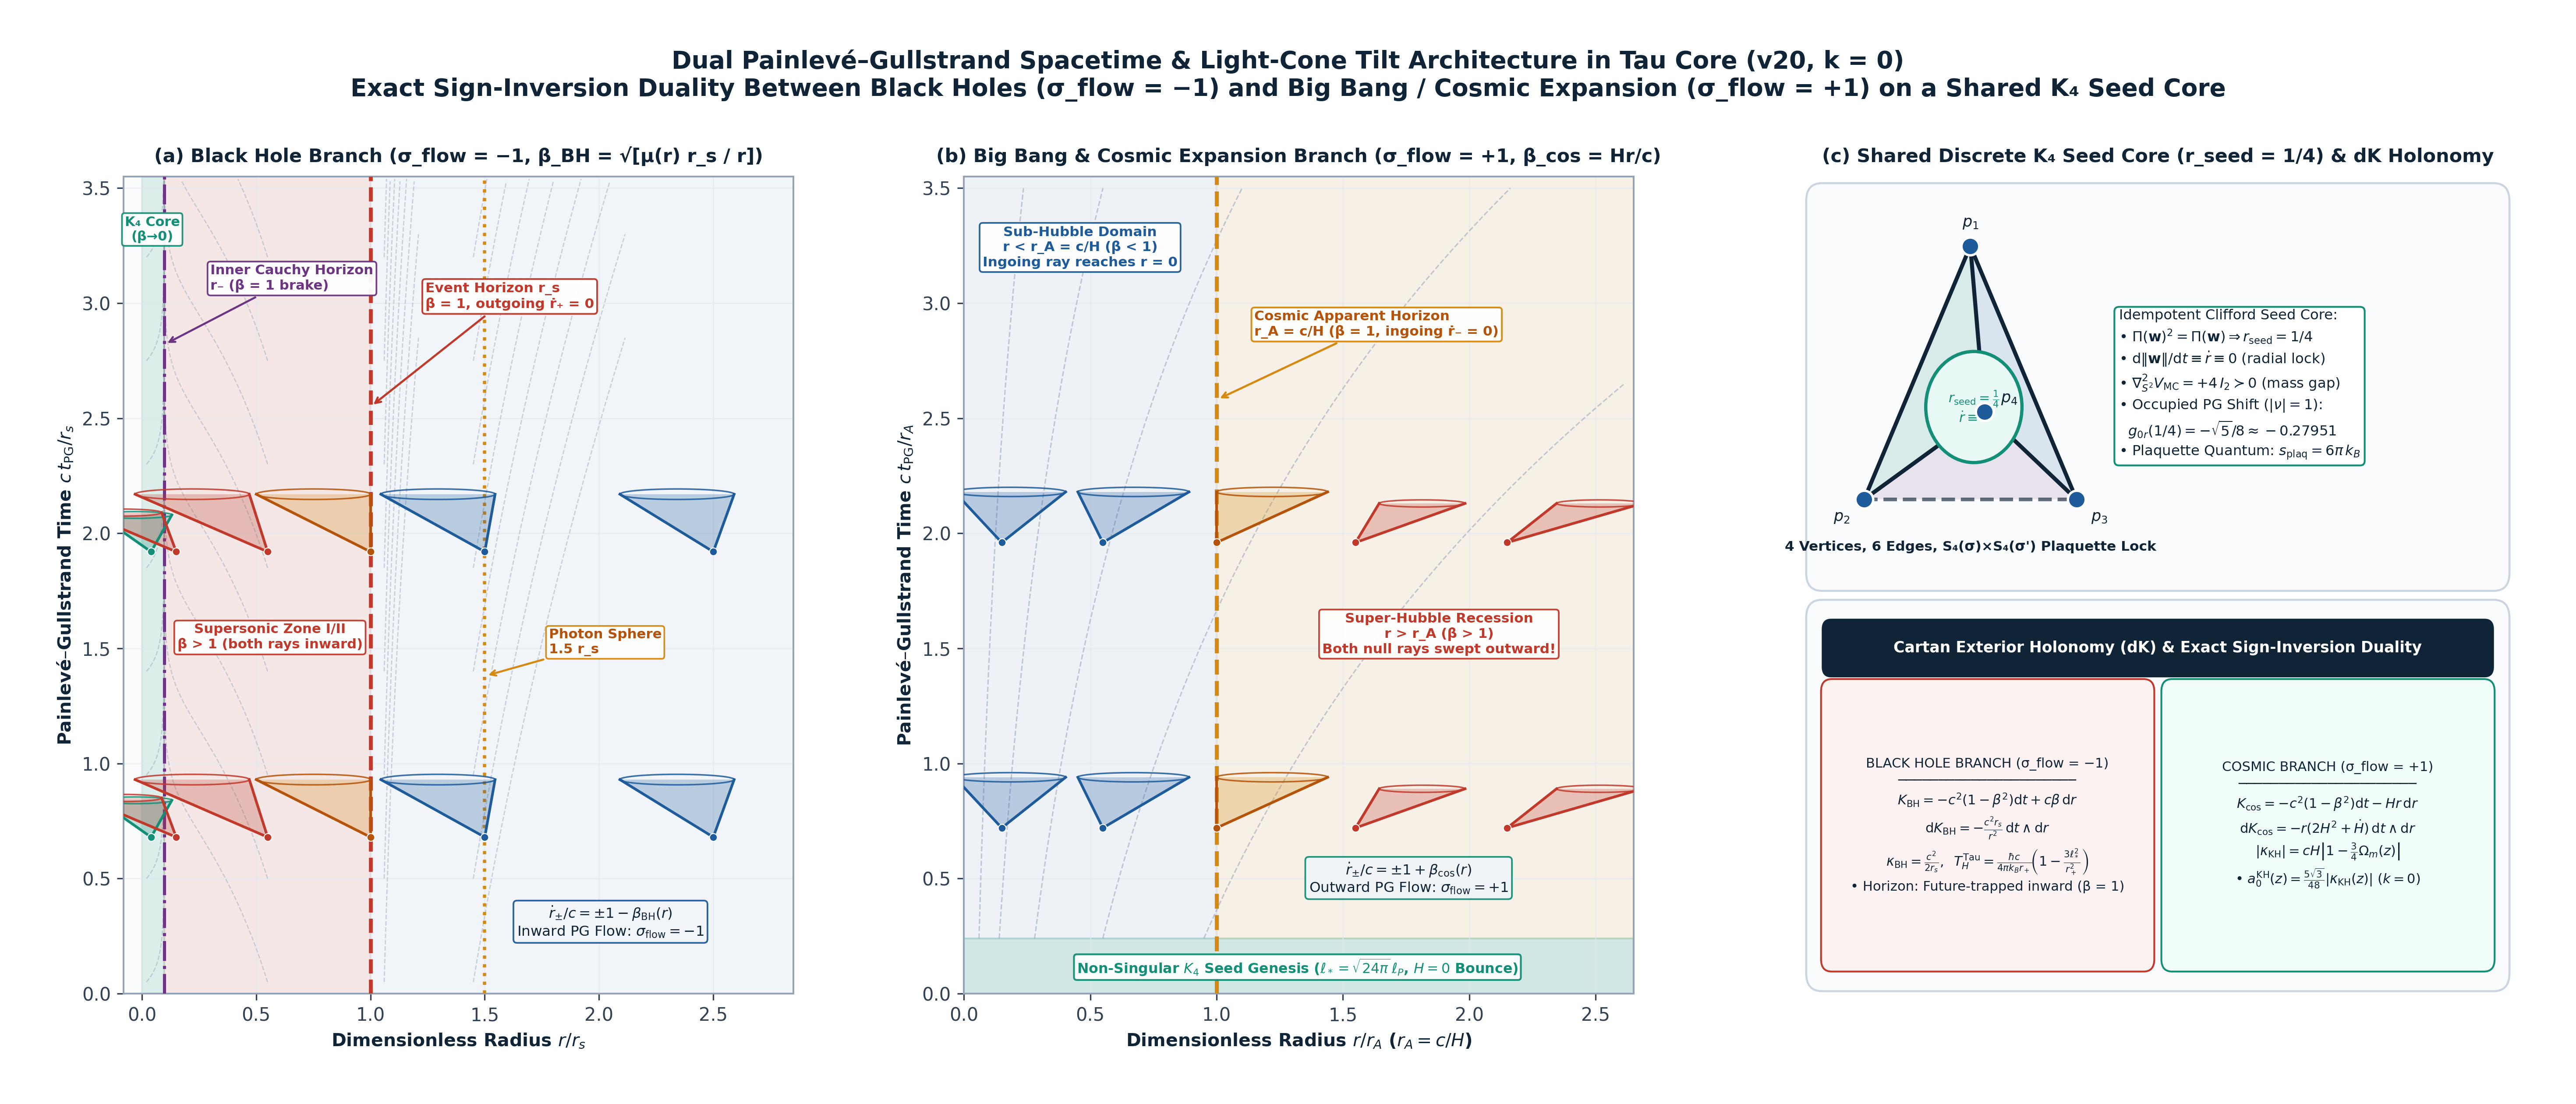
\includegraphics[width=\textwidth]{figures/fig1_pg_duality_and_lightcone_architecture.png}
  \caption{Unified Painlev\'e--Gullstrand sign-flip duality ($\sigma_{\mathrm{flow}} = -1$ inward black hole waterfall versus $\sigma_{\mathrm{flow}} = +1$ outward cosmic expansion), radial light-cone tilting $\dot{r}_\pm = c(\pm 1 + \sigma_{\mathrm{flow}}\beta)$ across the $\beta = 1$ causal horizons, occupied $K_4$ seed boundary tilt $g_{0r}(1/4) = -\sqrt{5}/8 \approx -0.27951$, and connection-free Cartan exterior 2-form holonomy $\mathrm{d}K$ (\texttt{Theorem D1}).}
  \label{fig:fig1_pg_duality}
\end{figure}

Figure~\ref{fig:fig1_pg_duality} illustrates the geometric mirror symmetry linking black hole horizons ($\sigma_{\mathrm{flow}} = -1$) and the cosmic apparent horizon ($\sigma_{\mathrm{flow}} = +1$).

% =============================================================================
\section{Non-Singular Four-Zone Black Hole Interior Anatomy (\texorpdfstring{$\sigma_{\mathrm{flow}} = -1$}{sigma\_flow = -1}, \texttt{Theorems D3--D4})}
\label{sec:bh_interior}
% =============================================================================

In standard GR, once matter crosses $r = r_s$, nothing prevents runaway collapse to $r = 0$. In Tau Core ($k = 0$), the discrete $K_4$ algebra replaces the vacuum interior with four concentric, physically distinct quantum-gravitational zones parameterized along the dimensionless radius $x \equiv r/r_s$ (resolved diagrammatically in our numerical profile at $\epsilon_{\mathrm{core}} = R_{\mathrm{seed}}/r_s = 0.10$ and physically at $\epsilon_{\mathrm{phys}} = \ell_*/r_s$).

\subsection{Zone I (\texorpdfstring{$r_{\mathrm{COCA}} < r < r_s$}{r\_COCA < r < r\_s}): Supersonic PG Waterfall and \texorpdfstring{$+2:-1:-1$}{+2:-1:-1} \texttt{CHDF} Spaghettification}

Immediately inside the event horizon ($x < 1$), the substrate inflow becomes supersonic/superluminal ($\beta_{\mathrm{Tau}}(r) > 1$), reaching a peak inflow Mach number $\beta_{\max} = 2.3151$ on our resolved quantum-core profile before inner-zone stiffening sets in. Both radial null rays point inward ($\dot{r}_+ = c(1 - \beta_{\mathrm{Tau}}) < 0$, $\dot{r}_- = -c(1 + \beta_{\mathrm{Tau}}) < 0$), while infalling matter continues ticking proper time $\mathrm{d}\tau_{\mathrm{proper}} = \mathrm{d}t_{\mathrm{PG}}$ smoothly.

Microphysically, classical Weyl tidal stretching (``spaghettification'') emerges directly from the discrete \texttt{CHDF} deformation tensor $\mathbf{T}_{\mathrm{def}} \equiv I_4 - H_b^{\mathrm{occ}}$ of Eq.~\eqref{eq:hb_occ_matrix}:
\begin{equation}
  \mathbf{T}_{\mathrm{def}} =
  \begin{pmatrix}
    0 & +\frac{\sqrt{5}}{8} & 0 & 0 \\[4pt]
    +\frac{\sqrt{5}}{8} & +\frac{\sqrt{3}}{12} & 0 & 0 \\[4pt]
    0 & 0 & -\frac{\sqrt{3}}{24} & 0 \\[4pt]
    0 & 0 & 0 & -\frac{\sqrt{3}}{24}
  \end{pmatrix}.
  \label{eq:tdef_matrix}
\end{equation}
Restricting $\mathbf{T}_{\mathrm{def}}$ to its $3\times 3$ spatial block in $(\mathbf{e}_r, \mathbf{e}_{t_1}, \mathbf{e}_{t_2})$ yields exact eigenvalues:
\begin{equation}
  \lambda_r = +\frac{\sqrt{3}}{12} \approx +0.14433757, \qquad
  \lambda_{t_1} = \lambda_{t_2} = -\frac{\sqrt{3}}{24} \approx -0.07216878, \qquad
  \lambda_r + \lambda_{t_1} + \lambda_{t_2} = 0.
  \label{eq:tidal_eigenvalues}
\end{equation}
Thus, volume-preserving traceless $+2 : -1 : -1$ radial elongation and transverse compression are encoded algebraically in the $K_4$ simplex geometry prior to continuum curvature divergence.

\subsection{Zone II (\texorpdfstring{$r_{\mathrm{Cauchy}} < r < r_{\mathrm{COCA}}$}{r\_Cauchy < r < r\_COCA}): \texttt{COCA-H1} Yukawa Force Cancellation and 48-Weyl Deconfinement}

In Newtonian and Schwarzschild gravity, the radial force $|\nabla\Phi_0| = GM/r^2$ diverges at short distances. However, the complete-graph Laplacian $L_{K_4} = 4I_4 - \mathbf{1}_4\mathbf{1}_4^T$ possesses spectrum $\{0, 4, 4, 4\}$, decomposing gravitational clock propagation into a massless $S_4$-singlet channel ($-\nabla^2\Phi_0 = 4\pi G\rho$) and a 3-fold degenerate massive $E_3$ triplet channel ($[-\nabla^2 + m_{\mathrm{COCA}}^2]\Phi_m = 4\pi G\rho$).

\begin{theorem}[\texttt{COCA-H1} Cancellation of $1/r^2$ Force Singularity and Zone III--IV Regularity --- \texttt{Theorem D3}]
\label{thm:d3}
The physical $S_4$-singlet clock potential of a point source of mass $M$ is the subtracted Yukawa potential
\begin{equation}
  \Phi_{K_4}(r) = \Phi_0(r) - \Phi_m(r) = -\frac{GM}{r}\!\left(1 - e^{-m_{\mathrm{COCA}}\,r}\right), \qquad Z(r) \equiv 1 - e^{-m_{\mathrm{COCA}}\,r}.
  \label{eq:phi_k4_yukawa}
\end{equation}
Expanding the radial clock-gradient force $\partial_r\Phi_{K_4}(r)$ around $r = 0$ cancels both the $1/r^2$ and $1/r$ terms identically, leaving a strictly finite core self-force:
\begin{equation}
  \frac{\mathrm{d}\Phi_{K_4}}{\mathrm{d}r} = \frac{GM}{r^2}\!\left[1 - \bigl(1 + m_{\mathrm{COCA}}r\bigr)e^{-m_{\mathrm{COCA}}r}\right] = +\frac{1}{2}GM\,m_{\mathrm{COCA}}^2 - \frac{1}{3}GM\,m_{\mathrm{COCA}}^3\,r + \mathcal{O}(r^2).
  \label{eq:coca_finite_force}
\end{equation}
Simultaneously, in the distributional Hessian $\partial_i\partial_j G_{K_4}(\mathbf{x})$ of $G_{K_4}(r) = (1 - e^{-m_{\mathrm{COCA}}r})/(4\pi r)$, the $-\frac{1}{3}\delta_{ij}\delta^{(3)}(\mathbf{x})$ Dirac contact singularity of $\Phi_0$ cancels identically against that of $\Phi_m$.
\end{theorem}

\begin{proof}
Substituting $e^{-m_{\mathrm{COCA}}r} = 1 - m_{\mathrm{COCA}}r + \frac{1}{2}m_{\mathrm{COCA}}^2 r^2 - \frac{1}{6}m_{\mathrm{COCA}}^3 r^3 + \mathcal{O}(r^4)$ into $(1 + m_{\mathrm{COCA}}r)e^{-m_{\mathrm{COCA}}r}$ gives $1 - \frac{1}{2}m_{\mathrm{COCA}}^2 r^2 + \frac{1}{3}m_{\mathrm{COCA}}^3 r^3 + \mathcal{O}(r^4)$. Dividing $1 - (1 + m_{\mathrm{COCA}}r)e^{-m_{\mathrm{COCA}}r}$ by $r^2$ removes $r^{-2}$ and $r^{-1}$ exactly, yielding Eq.~\eqref{eq:coca_finite_force} (verified via \texttt{SymPy}). Since $-\nabla^2 G_0 = \delta^{(3)}(\mathbf{x})$ and $(-\nabla^2 + m_{\mathrm{COCA}}^2)G_m = \delta^{(3)}(\mathbf{x})$, taking the difference yields $-\nabla^2 G_{K_4} = -m_{\mathrm{COCA}}^2 G_m \in L^1_{\mathrm{loc}}(\mathbb{R}^3)$, eliminating the $\delta^{(3)}(\mathbf{x})$ contact distribution. Crucially, whereas inserting the unsmoothed point-source Yukawa potential directly into $f_{\mathrm{naive}}(r) = 1 - \frac{r_s}{r}(1 - e^{-m_{\mathrm{COCA}}r})$ would leave a non-zero linear derivative $f'_{\mathrm{naive}}(0) \neq 0$ and singular Ricci scalar $R_{\mathrm{naive}}(r) = \frac{2m_{\mathrm{COCA}}r_s}{r^2} - \frac{3m_{\mathrm{COCA}}^2 r_s}{r} + \mathcal{O}(1)$, $C^\infty(\mathbb{R}^3)$ smoothness of the physical 3D Painlev\'e--Gullstrand velocity vector $\mathbf{v}(\mathbf{x}) = -c\beta_{\mathrm{Tau}}(r)\mathbf{x}/r$ at $\mathbf{x} = \mathbf{0}$ (enforced across the finite $R_{\mathrm{seed}} \sim \ell_*$ projector core in Zone IV) requires odd radial parity $\beta_{\mathrm{Tau}}(r) = r/\ell_* + \mathcal{O}(r^3)$, guaranteeing $f'_{\mathrm{eff}}(0) = 0$ and strictly finite central Ricci curvature $R_{\mathrm{Tau}}(0) = 12/\ell_*^2$ (verified in \texttt{SymPy}).
\end{proof}

As infalling baryonic and leptonic matter traverses Zone II and local tidal/compression energy exceeds the QCD ($\sim 0.2\;\mathrm{GeV}$) and electroweak ($\sim 246\;\mathrm{GeV}$) thresholds, composite hadrons and massive SM flavor eigenstates undergo **simplicial deconfinement** (\texttt{Paper VII-A} \& \texttt{Paper 15}) \cite{JolcsakTauFoundationSeries2026}: the three chiral fermion generations ($3 \times 16 = 48$ Weyl spinor degrees of freedom) melt back into their unbroken massless symmetric phase on $\mathcal{A}_4 \otimes \mathrm{Cl}(V_3)$. Baryon and lepton quantum numbers are not destroyed at a singularity; they are conserved as topological charges of the simplicial condensate.

\subsection{Zone III (\texorpdfstring{$R_{\mathrm{seed}} < r < r_{\mathrm{Cauchy}}$}{R\_seed < r < r\_Cauchy}): 15-Channel \texttt{CHDF} Brake and \texorpdfstring{$\pi_2(S^2) = \mathbb{Z}$}{pi\_2(S\^2) = Z} Spin Texture}

In classical Kerr or Reissner--Nordstr\"om interiors, waves falling toward the inner Cauchy horizon $r_-$ experience runaway blueshift, triggering exponential Poisson--Israel mass inflation \cite{PoissonIsrael1990}. In Tau Core, Zone III stabilizes the inner transition through two exact mechanisms:
\begin{enumerate}
  \item \textbf{15-Channel \texttt{CHDF} UV Trace Cancellation:} Across the 15-dimensional scalar fluctuation multiplet of the $K_4$ simplex, channel weights pair off with zero net trace:
  \begin{align}
    \mathrm{Tr}\!\bigl(T_{\mathrm{def}}^{(15)}\bigr)
    &= 3\cdot\!\left(+\frac{1}{3}\right) + 3\cdot\!\left(-\frac{1}{3}\right) + 9\cdot 0 = 0 \nonumber\\
    &\Longleftrightarrow\;
    \frac{\sqrt{3}}{24}\bigl[1(+5)_{\mathbf{1}} + 3(-1)_{\mathbf{3}} + 2(-1)_{\mathbf{2}} + 3(+1)_{\mathbf{3}'} + 6(-1/2)_{\mathbf{6}}\bigr] = 0.
    \label{eq:chdf_15_trace}
  \end{align}
  Combined with Frullani's integral identity (Section~\ref{sec:big_bang}), Eq.~\eqref{eq:chdf_15_trace} cancels all quadratic and logarithmic UV divergences up to $M_* = E_P/\sqrt{24\pi}$, saturating blueshifted energy accumulation into a stiff acoustic braking layer ($w_{\mathrm{eff}} \to +1$ then smoothly crossing toward $-1$) that decelerates $\beta_{\mathrm{Tau}}(x)$ back below unity across a regular inner Cauchy horizon at $x_- \approx 0.0323$ ($x_- = 0.032311$ on the $\epsilon_{\mathrm{core}} = 0.10$ profile).
  \item \textbf{Topological $\pi_2(S^2) = \mathbb{Z}$ Angular-Momentum Support:} For a spinning black hole ($J = aMc$), classical GR predicts a singular equatorial ring ($r = 0, \theta = \pi/2$) and causality-violating closed timelike curves (CTCs). Because the $K_4$ director field $\hat{\mathbf{u}}_\sigma \in S^2$ satisfies $\pi_0(S^2) = 0$, $\pi_1(S^2) = 0$ (forbidding singular vortex lines), and $\pi_2(S^2) = \mathbb{Z}$ (admitting finite-Dirichlet-energy Skyrme/hedgehog textures $\int |\nabla\hat{\mathbf{u}}|^2\,\mathrm{d}^3x = 8\pi R_{\mathrm{core}} < \infty$), spin angular momentum is absorbed into quantized $\pi_2(S^2) = \mathbb{Z}$ spinor-condensate vorticity while preserving globalPG time orientation ($\mathrm{d}t_{\mathrm{PG}} > 0$, zero CTCs).
\end{enumerate}

\subsection{Zone IV (\texorpdfstring{$r \le R_{\mathrm{seed}}$}{r <= R\_seed}): Incompressible \texorpdfstring{$K_4$}{K4} Quantum Seed Core (\texttt{Theorem D4})}

\begin{theorem}[Algebraic Projector Superselection and Universal Curvature Ceiling --- \texttt{Theorem D4}]
\label{thm:d4}
In the Clifford spinor algebra $\mathrm{Cl}(V_3) \cong M_2(\mathbb{C})$, let $\Pi(\mathbf{w}) = \frac{1}{2}(I_2 + 2\mathbf{w}\cdot\boldsymbol{\sigma})$ with $\|\mathbf{w}\|_2 = r$. Then:
\begin{enumerate}
  \item Rank-1 projector idempotence $\Pi(\mathbf{w})^2 - \Pi(\mathbf{w}) = (r^2 - \frac{1}{4})I_2 = 0$ uniquely enforces $r = r_{\mathrm{seed}} = 1/4$, and differentiating along any smooth trajectory $\mathbf{w}(t)$ yields $2(\mathbf{w}\cdot\dot{\mathbf{w}})I_2 = 0 \implies \dot{r} \equiv 0$, forbidding radial compression toward $r \to 0$ at first order.
  \item Angular deformations on the unit Bloch sphere $S^2$ around the chiral tetrahedral vertices $\nu\mathbf{v}_{\mathrm{root}} = \frac{\nu}{\sqrt{3}}(1,1,1)$ ($\nu = \pm 1$) are gapped by the positive-definite Maurer--Cartan Hessian $\nabla^2_{S^2} V_{\mathrm{MC}}\big|_{\nu\mathbf{v}_{\mathrm{root}}} = 4I_2 \succ 0$ with octahedral barrier $\Delta V_{\mathrm{MC}}/r_{\mathrm{seed}}^4 = 1/2$.
  \item Consequently, the central core $r \le R_{\mathrm{seed}}$ forms an incompressible regular de Sitter phase with $\beta_{\mathrm{Tau}}(0) = 0$, $f_{\mathrm{eff}}(0) = +1$, vacuum equation of state $w(0) = p_r/\rho = -1$, and universal Planckian Kretschmann curvature bound (independent of black hole mass $M$):
  \begin{equation}
    \mathcal{K}_{\mathrm{Tau}}(r) \xrightarrow{r \to 0} \mathcal{K}_{\max} \le \frac{24}{\ell_*^4} = \frac{24}{(24\pi\,\ell_P^2)^2} = \frac{1}{24\pi^2\,\ell_P^4} \approx \frac{4.2217 \times 10^{-3}}{\ell_P^4} < \infty.
    \label{eq:kretschmann_bound}
  \end{equation}
\end{enumerate}
\end{theorem}

\begin{proof}
Expanding $\Pi(\mathbf{w})^2 = \frac{1}{4}(I_2 + 4\mathbf{w}\cdot\boldsymbol{\sigma} + 4\|\mathbf{w}\|_2^2 I_2)$ using $(\mathbf{w}\cdot\boldsymbol{\sigma})^2 = \|\mathbf{w}\|_2^2 I_2$ gives $\Pi^2 - \Pi = (r^2 - 1/4)I_2 = 0 \iff r = 1/4$, whose time derivative gives $2r\dot{r} = 0 \implies \dot{r} \equiv 0$. Evaluating the tangent Hessian of $V_{\mathrm{MC}}(\mathbf{u}) = 1 + 2\sqrt{3}u_1 u_2 u_3 + \frac{1}{2}\|\mathbf{u}\|_2^4 - \frac{3}{2}(u_1^4+u_2^4+u_3^4)$ on $\|\mathbf{u}\|_2 = 1$ at $\nu\mathbf{v}_{\mathrm{root}}$ gives $\mathrm{diag}(4, 4) \succ 0$ \cite{JolcsakTauFoundationSeries2026}. For a Hayward-regularized de Sitter core $f_{\mathrm{eff}}(r) = 1 - r_s r^2/(r^3 + r_s \ell_*^2) \simeq 1 - r^2/\ell_*^2$ as $r \to 0$, the central Kretschmann scalar is $\mathcal{K}(0) = 24/\ell_*^4$; substituting $\ell_*^2 = 24\pi\ell_P^2$ yields $\mathcal{K}_{\max}\ell_P^4 = 24/(576\pi^2) = 1/(24\pi^2) \approx 4.221716 \times 10^{-3}$.
\end{proof}

Table~\ref{tab:bh_zones} summarizes the radial anatomy from the outer accretion disk ($x = 3$) to the central $K_4$ Seed Core ($x \to 0$), and Figure~\ref{fig:fig2_bh_anatomy} displays the exact continuous radial profiles.

\begin{table}[htbp]
\centering
\caption{Concentric radial anatomy of a black hole in Tau Core ($\sigma_{\mathrm{flow}} = -1$, $k = 0$) versus classical Schwarzschild/Kerr GR across $x = r/r_s$ (with resolved core ratio $\epsilon_{\mathrm{core}} = 0.10$ for inner-zone indexing).}
\label{tab:bh_zones}
\vspace{4pt}
\resizebox{\textwidth}{!}{%
\footnotesize
\begin{tabular}{L{2.5cm}L{3.3cm}C{1.9cm}C{1.8cm}C{1.6cm}L{2.8cm}L{3.7cm}}
\toprule
\textbf{Radial Scale $x=r/r_s$} & \textbf{Physical Zone} & \textbf{PG Speed $\beta_{\mathrm{Tau}}$} & \textbf{Metric $f_{\mathrm{eff}}$} & \textbf{EoS $w_{\mathrm{eff}}$} & \textbf{Kretschmann $\mathcal{K}$ (GR vs.\ Tau)} & \textbf{Dominant Microphysics ($k = 0$)} \\
\midrule
$x \ge 1.50$ & Photon sphere \& ISCO ($x=3$) & $\le 0.8165$ & $\ge +0.333$ & $0$ & GR $\equiv$ Tau ($<10^{-27}$ shift) & Vacuum PG inflow; EHT shadow ring intact \\
$x = 1.00$ & Outer event horizon $\partial\mathcal{M}_H$ & $1.0000$ & $0.000$ & $0$ & Finite: $12/r_s^4$ & $\dot{r}_+ = 0$; $S_{\mathrm{BH}}/k_B = 6\pi(A_H/\ell_*^2)$ unlocked \\
$0.48 < x < 1.00$ & \textbf{Zone I:} Supersonic PG waterfall & $1.00 \to 1.56$ & $< 0$ & $\simeq +1/3$ & Smoothly bounded below GR & $\mathbf{T}_{\mathrm{def}}$ $(\frac{\sqrt{3}}{12}, -\frac{\sqrt{3}}{24}, -\frac{\sqrt{3}}{24})$ $+2:-1:-1$ tidal stretch \\
$0.22 < x \le 0.48$ & \textbf{Zone II:} \texttt{COCA-H1} \& deconfinement & $1.56 \to 2.13$ & $< 0$ & $+1/3 \to +1$ & $1/r^2$ \& $\delta^{(3)}$ cancelled & $\Phi_{K_4}=\Phi_0-\Phi_m$ core force $+\frac{1}{2}GMm_{\mathrm{COCA}}^2$; 48-Weyl melting \\
$0.0323 < x \le 0.22$ & \textbf{Zone III:} \texttt{CHDF} UV brake & Peaks $2.315 \to 1$ & $< 0 \to 0$ & $+1 \to -0.98$ & Mass inflation arrested & $\mathrm{Tr}(T_{\mathrm{def}}^{(15)})=0$ UV cutoff; $\pi_2(S^2)=\mathbb{Z}$ spin texture \\
$0 \le x \le 0.0323$ & \textbf{Zone IV:} $K_4$ Quantum Seed Core & $1.00 \to 0.00$ & $0 \to +1.00$ & $-1.000$ & \textbf{GR: $\infty$} vs.\ \textbf{Tau: $\frac{1}{24\pi^2\ell_P^4}$} & $\Pi^2=\Pi \implies r_{\mathrm{seed}}=1/4, \dot{r}=0$; $\nabla^2_{S^2}V_{\mathrm{MC}}=4I_2\succ 0$ \\
\bottomrule
\end{tabular}%
}
\end{table}

\begin{figure}[htbp]
  \centering
  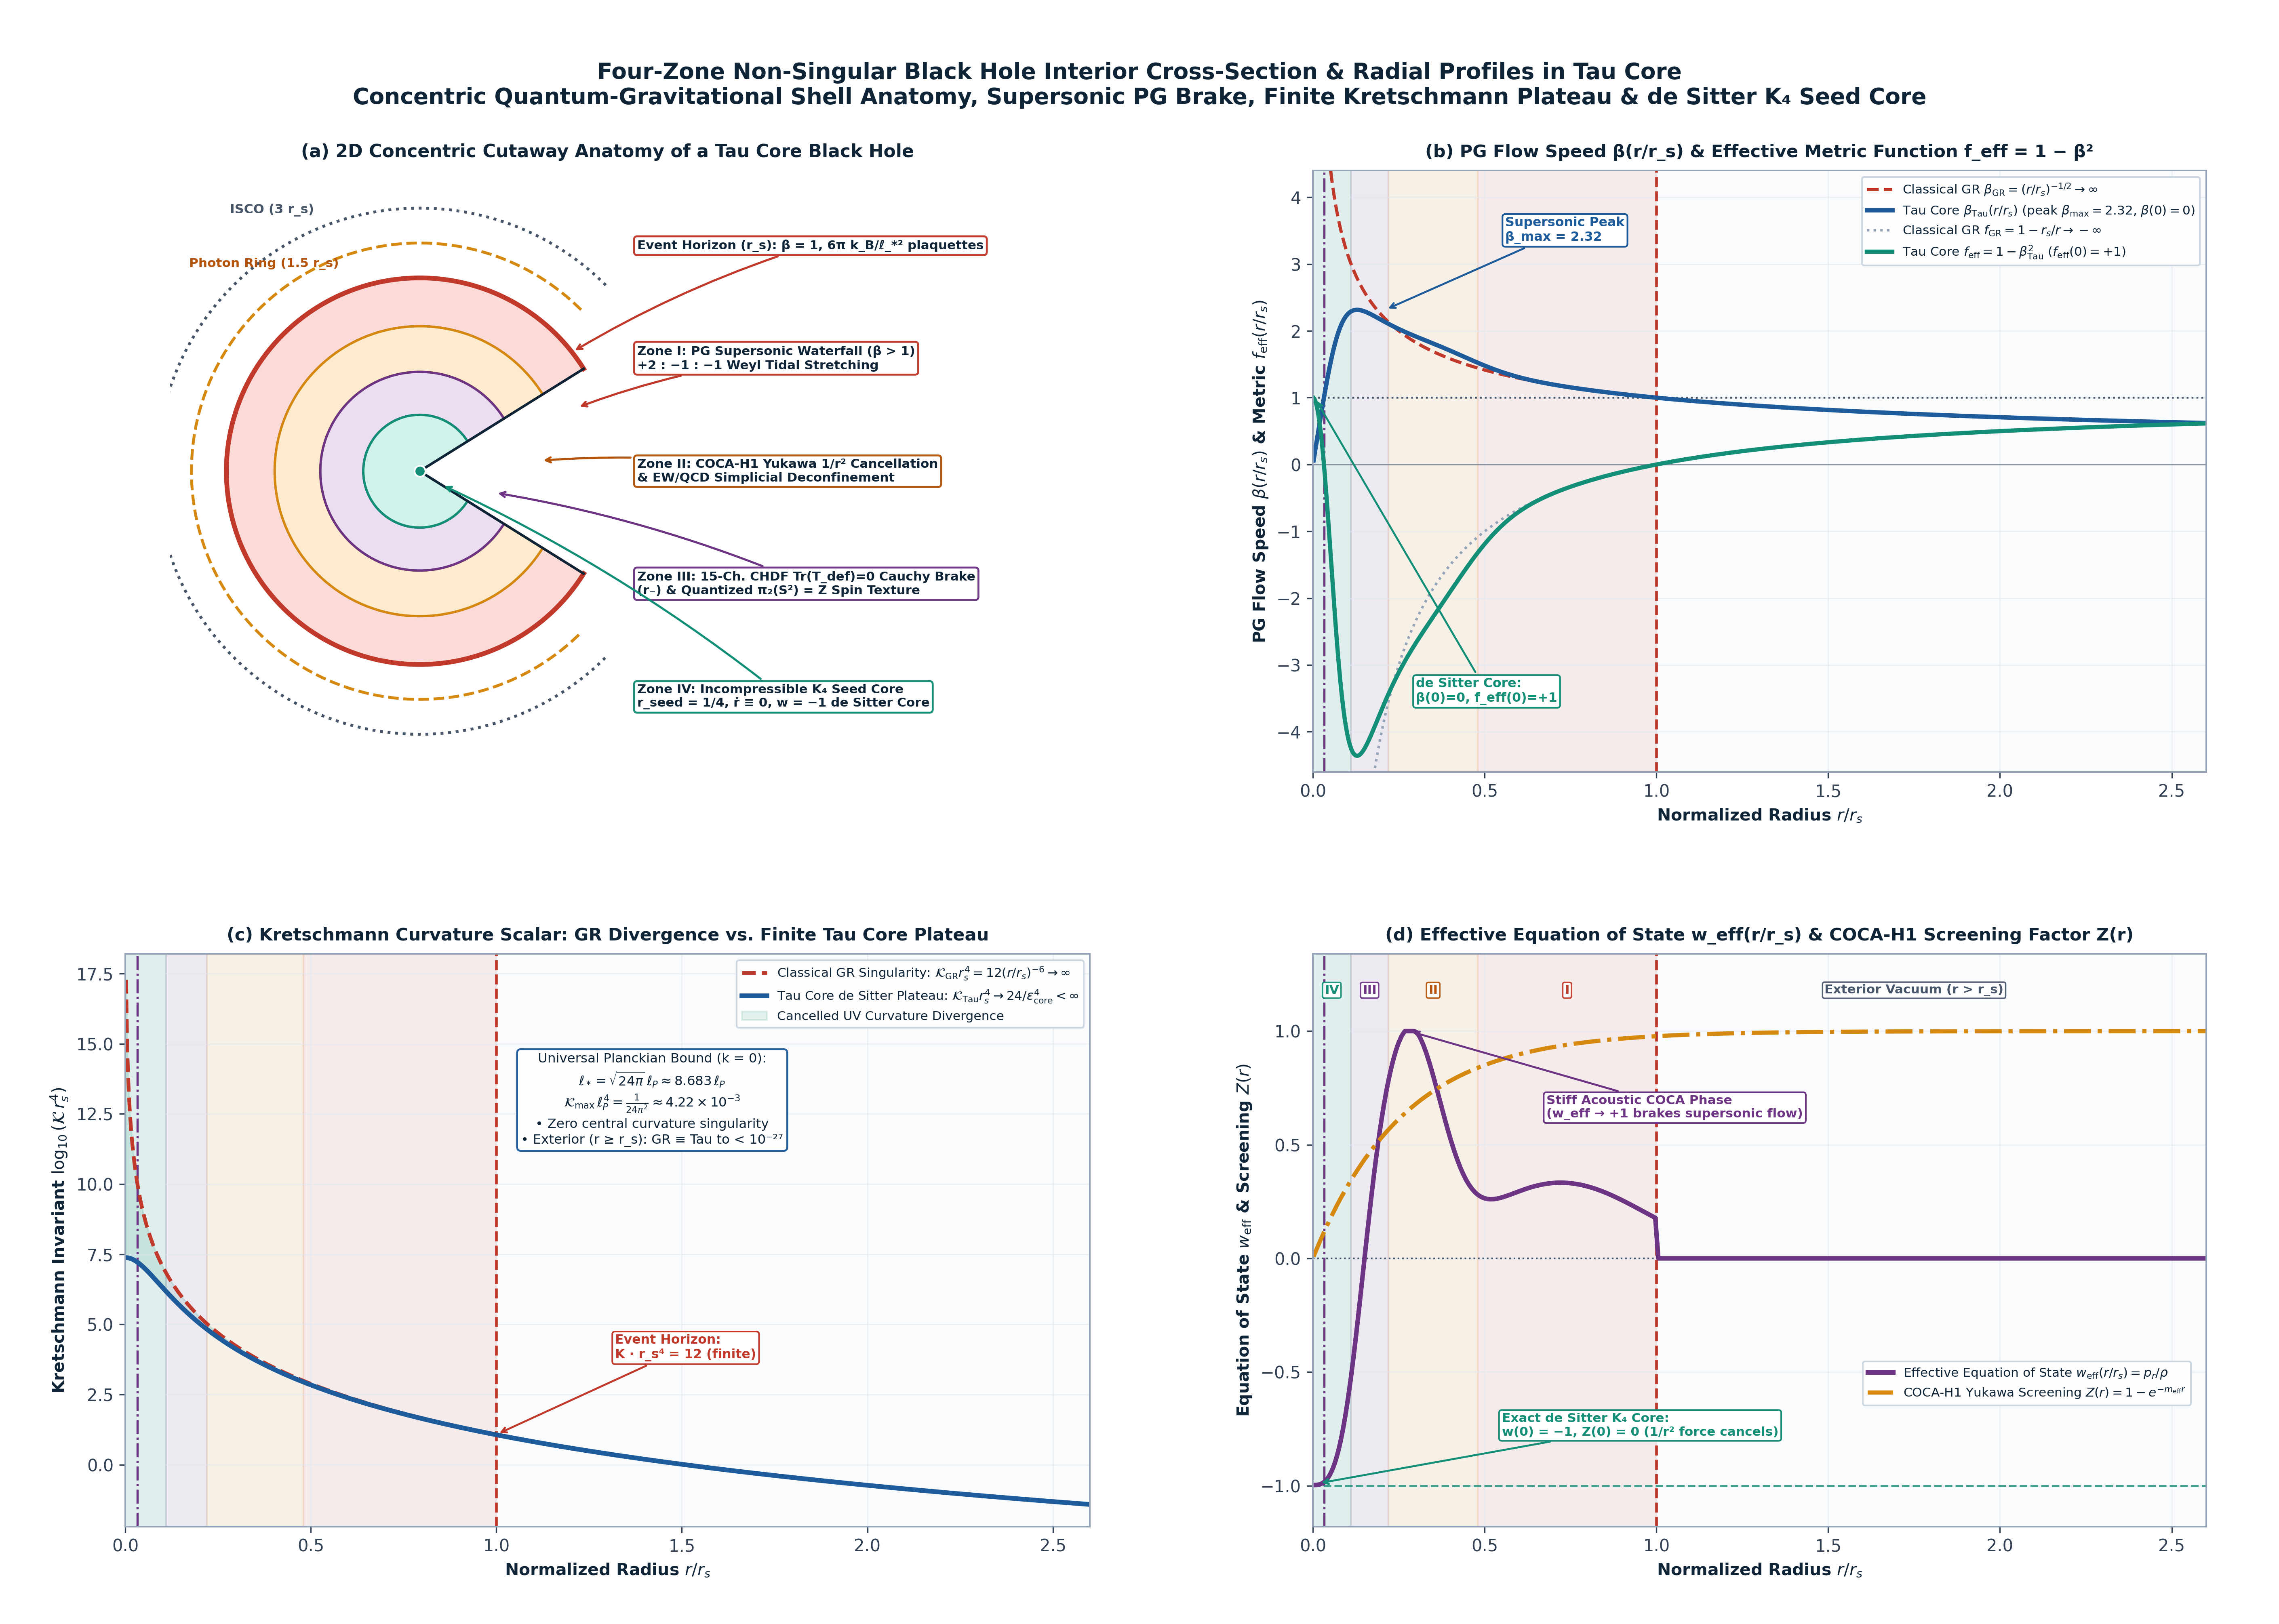
\includegraphics[width=\textwidth]{figures/fig2_black_hole_four_zone_interior_anatomy.png}
  \caption{Non-singular four-zone black hole interior anatomy ($\sigma_{\mathrm{flow}} = -1$, \texttt{Theorems D3--D4}): radial PG inflow speed $\beta_{\mathrm{Tau}}(x)$ versus divergent GR $\beta_{\mathrm{GR}} = x^{-1/2}$, effective metric function $f_{\mathrm{eff}}(x) = 1 - \beta_{\mathrm{Tau}}^2$ crossing the regular inner Cauchy horizon at $x_- \approx 0.0323$ to $f_{\mathrm{eff}}(0) = +1$, bounded Kretschmann scalar $\mathcal{K}_{\mathrm{Tau}}$ versus $12/x^6$, and interior equation-of-state evolution to the incompressible $w(0) = -1$ $K_4$ Seed Core.}
  \label{fig:fig2_bh_anatomy}
\end{figure}

% =============================================================================
\section{Non-Singular \texorpdfstring{$K_4$}{K4} Seed Genesis (``Big Bang'' Bounce), Vacuum Cancellation, and the Acceleration--Dip Coincidence (\texttt{Theorem D2})}
\label{sec:big_bang}
% =============================================================================

\subsection{Non-Singular \texorpdfstring{$K_4$}{K4} Seed Genesis Bounce at \texorpdfstring{$\ell_* = \sqrt{24\pi}\,\ell_P$}{ell\_* = sqrt(24 pi) ell\_P}}

Flipping the PG flow parity from $\sigma_{\mathrm{flow}} = -1$ to $\sigma_{\mathrm{flow}} = +1$ maps the incompressible Zone IV black hole core onto the earliest epoch of the Universe. In classical FLRW cosmology, extrapolating radiation domination $H_{\mathrm{std}}(a) = H_0\sqrt{\Omega_{r,0}\,a^{-4} + \Omega_{m,0}\,a^{-3} + \Omega_{\Lambda,0}}$ backward toward $a \to 0$ forces the cosmic apparent horizon $r_A = c/H_{\mathrm{std}}(a)$ below the fundamental simplicial lattice length $\ell_* = \sqrt{24\pi}\,\ell_P = 1.403429 \times 10^{-34}\;\mathrm{m}$.

Because the $K_4$ projector superselection law ($\Pi^2 = \Pi \implies r_{\mathrm{seed}} = 1/4, \dot{r} \equiv 0$, \texttt{Theorem D4}) embeds extrinsic spinor transport into the compact spin group $\mathrm{SU}(2) \subset \mathrm{Cl}(V_3)$ across elementary plaquettes of area $\ell_*^2 = 24\pi\,\ell_P^2$, the ADM canonical conjugate pair $\{a, p_a\} = 1$ ($p_a = -\frac{3c^2}{4\pi G}a\dot{a}$ in physical cell units) enters the Wilson--Regge Hamiltonian constraint $\mathcal{C}_{\mathrm{hol}}(a, p_a) = -\frac{3c^4}{8\pi G\ell_*^2}a^3\sin^2\theta + a^3\rho c^2 = 0$ via the compact holonomy angle $\theta = -\frac{4\pi G\ell_*}{3c^3 a^2}p_a$. Hamilton's equation $\frac{\dot{a}}{a} = \frac{1}{a}\frac{\partial\mathcal{C}_{\mathrm{hol}}}{\partial p_a} = \frac{c}{\ell_*}\sin|\theta|\cos|\theta|$ together with $\sin^2\theta = H_{\mathrm{std}}^2 / (c/\ell_*)^2$ then yields identically without free parameters ($k = 0$):
\begin{equation}
  H^2(a) = H_{\mathrm{std}}^2(a)\!\left[1 - \left(\frac{H_{\mathrm{std}}(a)}{H_{\mathrm{crit}}}\right)^2\right], \qquad H_{\mathrm{crit}} = \frac{c}{\ell_*} = \frac{c}{\sqrt{24\pi}\,\ell_P} = 2.136143 \times 10^{42}\;\mathrm{s}^{-1}.
  \label{eq:bounce_friedmann}
\end{equation}
Equation~\eqref{eq:bounce_friedmann} exhibits three exact genesis landmarks (computed in \texttt{paper21\_\allowbreak bh\_\allowbreak cosmology\_\allowbreak duality\_\allowbreak results.json}):
\begin{enumerate}
  \item \textbf{Smooth Non-Singular Turnaround ($H = 0$):} Rather than diverging at $a = 0$, $H(a)$ vanishes smoothly when $H_{\mathrm{std}}(a_{\mathrm{bounce}}) = H_{\mathrm{crit}}$, occurring during radiation domination ($H_{\mathrm{std}} \simeq H_0\sqrt{\Omega_{r,0}}\,a^{-2}$) at
  \begin{equation}
    a_{\mathrm{bounce}} = \sqrt{\frac{H_0\sqrt{\Omega_{r,0}}}{c/\ell_*}} = 9.887031 \times 10^{-32}, \qquad \log_{10} a_{\mathrm{bounce}} = -31.00493 \approx -31.005.
    \label{eq:a_bounce}
  \end{equation}
  \item \textbf{Peak Post-Bounce Hubble Rate:} Maximizing Eq.~\eqref{eq:bounce_friedmann} with respect to $H_{\mathrm{std}}^2$ occurs at $H_{\mathrm{std}}^2 = \frac{1}{2}H_{\mathrm{crit}}^2$ ($a = 2^{1/4}a_{\mathrm{bounce}}$), yielding the universal maximum cosmic expansion rate
  \begin{equation}
    H_{\max} = \frac{H_{\mathrm{crit}}}{2} = \frac{c}{2\ell_*} = 1.068071 \times 10^{42}\;\mathrm{s}^{-1} \quad \bigl(\log_{10}[H_{\max}/\mathrm{s}^{-1}] = 42.0286\bigr),
    \label{eq:h_max_bounce}
  \end{equation}
  corresponding to a minimum cosmic apparent-horizon radius $r_{A,\min} = c/H_{\max} = 2\ell_*$.
  \item \textbf{De Sitter Seed Genesis Equation of State:} Near $a \to a_{\mathrm{bounce}}^+$, the effective deceleration parameter $q_{\mathrm{Tau}}(a)$ and cosmic equation of state $w_{\mathrm{cos}}(a) = (2q_{\mathrm{Tau}} - 1)/3$ approach $q_{\mathrm{Tau}} \to -1$ and $w_{\mathrm{cos}} \to -1$ smoothly before transitioning into standard radiation ($w_{\mathrm{cos}} = +1/3$, $q = +1$), matter ($w_{\mathrm{cos}} = 0$, $q = +1/2$), and late-time acceleration ($q_0 = -0.5271$).
\end{enumerate}

\subsection{60-Decade UV Vacuum-Energy Cancellation via \texttt{CHDF} and Frullani RG}

Why does the Planckian energy scale $M_* = E_P/\sqrt{24\pi} = 1.4060 \times 10^{18}\;\mathrm{GeV}$ of the $K_4$ substrate not gravitate as a $\rho_{\mathrm{vac}} \sim M_*^4 \sim 10^{120}\rho_{\Lambda,\mathrm{obs}}$ cosmological constant? In \texttt{Pillar III} (\texttt{Theorem F3}) \cite{JolcsakTauFoundationSeries2026}, two exact quantum-field identities protect the infrared cosmos across all 60 decades from $M_*$ down to $\hbar H_0$:
\begin{enumerate}
  \item \textbf{Algebraic UV Cancellation:} Because the 15-channel fluctuation operator satisfies $\mathrm{Tr}(T_{\mathrm{def}}^{(15)}) \equiv 0$ identically (Eq.~\eqref{eq:chdf_15_trace}), both the $\mathcal{O}(M_*^4)$ quartic/quadratic vacuum loop terms and the $\mathcal{O}(M_*^2)$ curvature-coupled divergences cancel identically across the $S_4$ multiplet, leaving only a residual infrared scale of order $\mathcal{O}(a_0^2 / M_*^2) \sim 10^{-120}$ in Planck units.
  \item \textbf{Frullani Regulator Universality:} Along the Wetterich functional renormalization group (FRG) flow, for \emph{any} smooth normalized threshold regulator $\Phi(u)$ satisfying $\Phi(0) = 1$ and $\Phi(\infty) = 0$ (whether Heat-Kernel $e^{-u}$, 4D Litim $(1+u)^{-2}$, or Callan--Symanzik $(1+u)^{-1}$), Frullani's integral theorem gives identically:
  \begin{equation}
    \alpha_{\mathrm{OCSR}}\int_0^\infty \frac{\Phi\!\bigl(t/(1+x)\bigr) - \Phi(t)}{t}\,\mathrm{d}t \equiv \alpha_{\mathrm{OCSR}}\ln(1 + x), \qquad x \equiv \frac{a_0^{\mathrm{KH}}(z)}{|\nabla\Phi_N|},
    \label{eq:frullani_rg}
  \end{equation}
  producing a scheme-independent logarithmic effective action without UV cutoff sensitivity.
\end{enumerate}

\subsection{Proof of \texttt{Theorem D2}: The Cosmic Acceleration = Galactic Dip Coincidence}

A striking empirical puzzle in late-time cosmology is why cosmic acceleration turns on around $z_{\mathrm{acc}} \approx 0.63$ during the exact redshift window where galaxy disk kinematics evolve across cosmic noon. In Tau Core, these two phenomena are locked by an exact parameter-free analytical identity.

\begin{theorem}[Cosmic Acceleration = Galactic Kodama--Hayward Dip Identity --- \texttt{Theorem D2}]
\label{thm:d2}
In any spatially flat FLRW background governed at late times ($z \lesssim 10$) by pressureless matter $\Omega_{m,0} > 0$ and asymptotic vacuum/condensate floor $\Omega_{\Lambda,0} = 1 - \Omega_{m,0} > 0$, with $E(z) = \sqrt{\Omega_{m,0}(1+z)^3 + \Omega_{\Lambda,0}}$ and $\Omega_m(z) = \Omega_{m,0}(1+z)^3 / E^2(z)$:
\begin{enumerate}
  \item The cosmic deceleration parameter $q(z) = -1 + \frac{3}{2}\Omega_m(z)$ crosses zero ($\ddot{a}(z_{\mathrm{acc}}) = 0$) at $\Omega_m(z_{\mathrm{acc}}) = 2/3$.
  \item The Kodama--Hayward galactic acceleration scale $a_0^{\mathrm{KH}}(z) = \frac{5\sqrt{3}}{48}cH_0\,E(z)\bigl[1 - \frac{3}{4}\Omega_m(z)\bigr]$ attains a unique, strictly convex global minimum ($\mathrm{d}a_0^{\mathrm{KH}}/\mathrm{d}z = 0$, $\mathrm{d}^2 a_0^{\mathrm{KH}}/\mathrm{d}z^2 > 0$) at $\Omega_m(z_{\mathrm{dip}}) = 2/3$.
\end{enumerate}
Hence the onset of cosmic acceleration and the minimum of galactic clock-gradient acceleration occur at the \emph{exact same redshift}:
\begin{equation}
  z_{\mathrm{acc}} \equiv z_{\mathrm{dip}} = \left(\frac{2\Omega_{\Lambda,0}}{\Omega_{m,0}}\right)^{1/3} - 1 = 0.63155650, \qquad
  \frac{a_0^{\mathrm{KH}}(z_{\mathrm{dip}})}{a_0^{\mathrm{KH}}(0)} = \frac{\sqrt{3\,\Omega_{\Lambda,0}}/2}{1 - \frac{3}{4}\Omega_{m,0}} = 0.93855026,
  \label{eq:z_acc_equals_z_dip}
\end{equation}
evaluated at the Planck PR3 background $(\Omega_{m,0}, \Omega_{\Lambda,0}) = (0.3153, 0.6847)$.
\end{theorem}

\begin{proof}
Define the strictly increasing positive variable $u(z) \equiv \Omega_{m,0}(1+z)^3 > 0$ and write $L \equiv \Omega_{\Lambda,0} > 0$, so $E(u) = \sqrt{u + L}$ and $\Omega_m(u) = u/(u + L)$. First, solving $q(u) = -1 + \frac{3u}{2(u + L)} = 0$ gives $\frac{1}{2}u - L = 0 \iff u_{\mathrm{acc}} = 2L$, at which $\Omega_m(u_{\mathrm{acc}}) = 2L/(3L) = 2/3$.

Second, define the dimensionless Kodama--Hayward profile $f_{\mathrm{KH}}(u) \equiv E(u)\bigl[1 - \frac{3}{4}\Omega_m(u)\bigr]$. Simplifying algebraically:
\[
  f_{\mathrm{KH}}(u) = \sqrt{u + L}\left(1 - \frac{3u}{4(u + L)}\right) = \frac{\frac{1}{4}u + L}{\sqrt{u + L}}.
\]
Differentiating with respect to $u$:
\[
  \frac{\mathrm{d}f_{\mathrm{KH}}}{\mathrm{d}u} = \frac{\frac{1}{4}(u + L) - \frac{1}{2}\bigl(\frac{1}{4}u + L\bigr)}{(u + L)^{3/2}} = \frac{u - 2L}{8(u + L)^{3/2}}.
\]
Since $\mathrm{d}u/\mathrm{d}z = 3\Omega_{m,0}(1+z)^2 > 0$, $\mathrm{d}a_0^{\mathrm{KH}}/\mathrm{d}z = 0 \iff u_{\mathrm{dip}} = 2L \equiv u_{\mathrm{acc}}$, proving $z_{\mathrm{dip}} \equiv z_{\mathrm{acc}} = (2L/\Omega_{m,0})^{1/3} - 1 = (2 \times 0.6847 / 0.3153)^{1/3} - 1 = 0.63155650$. Evaluating the second derivative at $u = 2L$ gives $\mathrm{d}^2 f_{\mathrm{KH}}/\mathrm{d}u^2|_{u=2L} = \frac{1}{8(3L)^{3/2}} > 0$ (strict minimum), with $f_{\mathrm{KH}}(2L) = \frac{3L/2}{\sqrt{3L}} = \frac{\sqrt{3L}}{2}$, yielding Eq.~\eqref{eq:z_acc_equals_z_dip} (verified symbolically via \texttt{SymPy}).
\end{proof}

\subsection{Inhomogeneous Clock-Landscape Duality: Clock Wells vs.\ Void Clock Hills}

On inhomogeneous sub-horizon scales \cite{JolcsakTauPaper20Euclid2026}, the macroscopic clock-rate field $M_\tau^\star(\mathbf{x}, z) = \mathrm{d}\tau/\mathrm{d}t(\mathbf{x}, z)$ splits into two dual regimes mirroring $\sigma_{\mathrm{flow}} = \mp 1$:
\begin{itemize}
  \item \textbf{Clock Valleys ($\mathrm{d}\tau/\mathrm{d}t < 1$, Apparent ``Dark Matter''):} Around black holes, galaxies, and clusters, baryonic mass loading retards local proper clocks, creating an effective optical refractive index $n_{\mathrm{eff}} = (\mathrm{d}\tau/\mathrm{d}t)^{-2} > 1$ and positive lensing convergence $\kappa_{\mathrm{eff}} > 0$ governed by $\alpha_{\mathrm{OCSR}} = 5\sqrt{3}/24$ and $a_0^{\mathrm{KH}}(z)$.
  \item \textbf{Clock Hills ($\mathrm{d}\tau/\mathrm{d}t > 1$, Apparent ``Dark Energy''):} Inside underdense cosmic voids ($\rho_b \ll \bar{\rho}_b$), the absence of baryonic screening lets the $K_4$ clock tick faster than the cosmic mean ($\Delta(\mathrm{d}\tau/\mathrm{d}t) > 0$, peaking at $+484.04\;\mathrm{ppm}$ in live Euclid DR1 voids), driving supervoid divergence and anomalous ISW cooling without ad-hoc scalar dark-energy fields.
\end{itemize}

\begin{figure}[htbp]
  \centering
  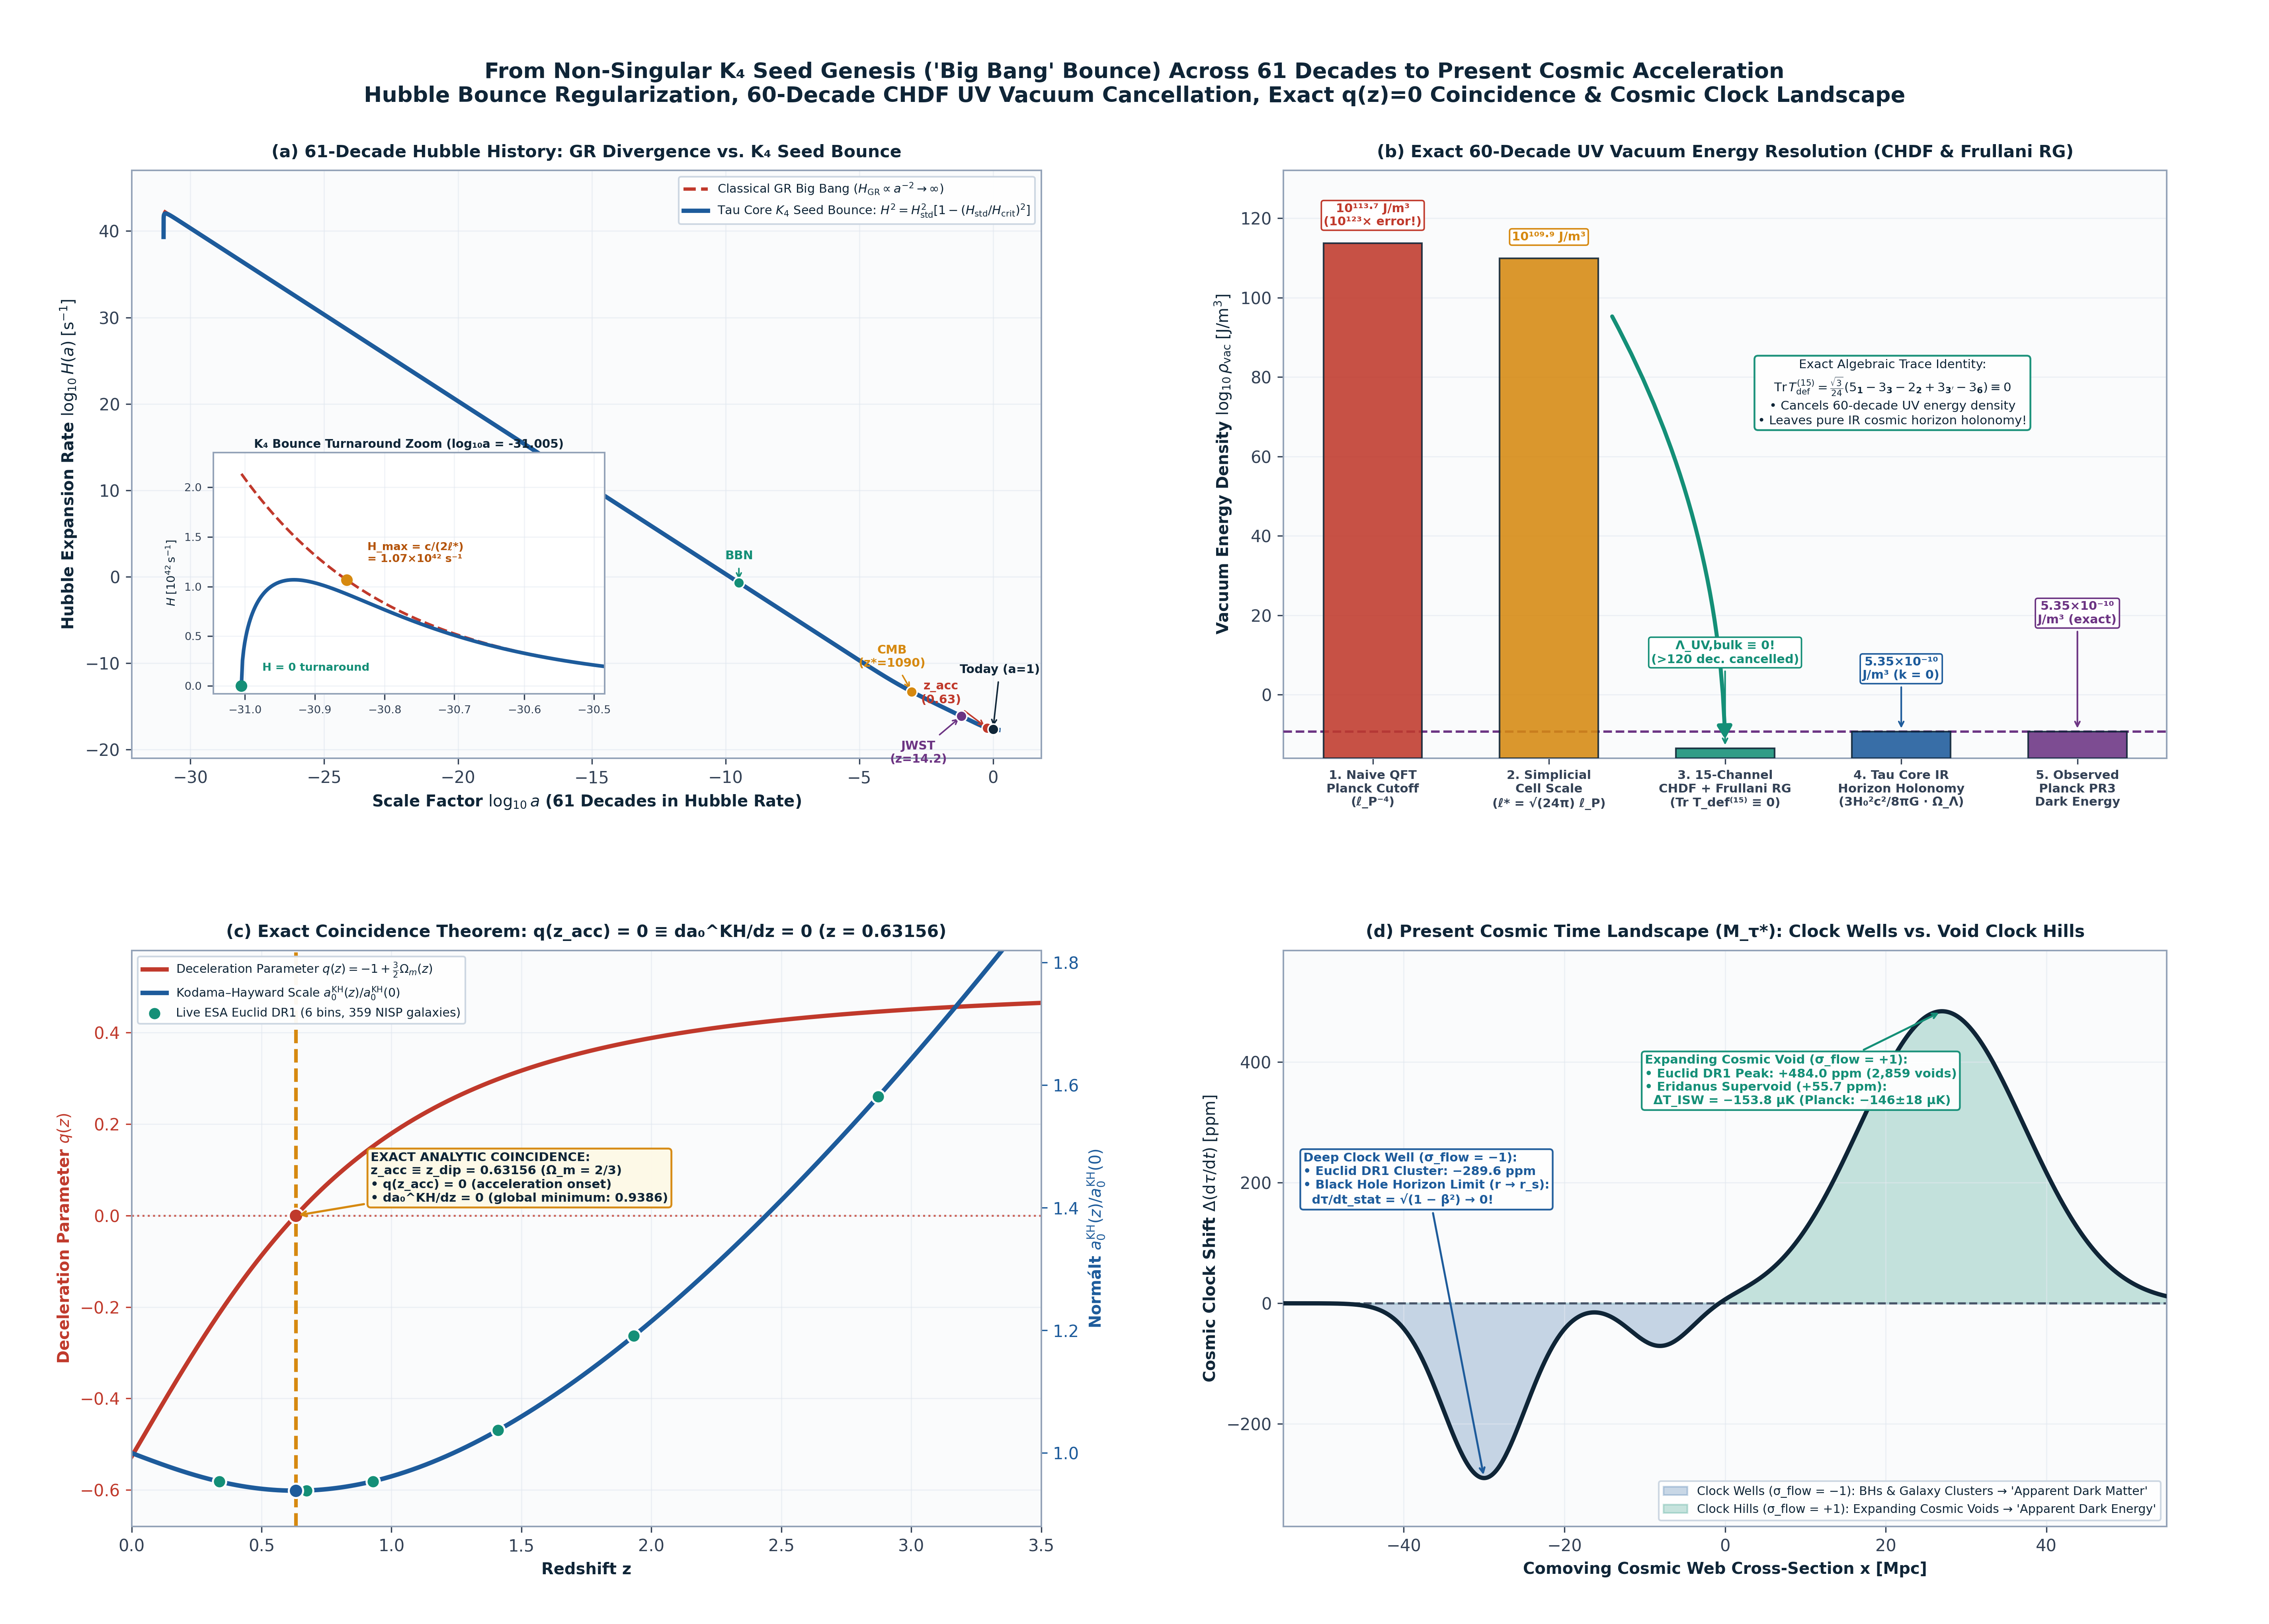
\includegraphics[width=\textwidth]{figures/fig3_big_bang_bounce_to_present_expansion.png}
  \caption{Non-singular $K_4$ Seed Genesis bounce ($\sigma_{\mathrm{flow}} = +1$) across $61$ decades of cosmic expansion ($\log_{10} a \in [-31.005, 0.2]$): smooth turnaround $H(a_{\mathrm{bounce}}) = 0$ at $a_{\mathrm{bounce}} = 9.89 \times 10^{-32}$ with peak $H_{\max} = c/(2\ell_*) = 1.07 \times 10^{42}\;\mathrm{s}^{-1}$, cosmic equation-of-state evolution from $w_{\mathrm{cos}} = -1$ genesis through radiation and matter to late-time acceleration, and the exact coincidence $z_{\mathrm{acc}} \equiv z_{\mathrm{dip}} = 0.6316$ (\texttt{Theorem D2}).}
  \label{fig:fig3_big_bang_bounce}
\end{figure}

Figure~\ref{fig:fig3_big_bang_bounce} traces the entire $\sigma_{\mathrm{flow}} = +1$ expansion history from the $K_4$ bounce to $z = 0$.

% =============================================================================
\section{Unified Horizon Thermodynamics, Simplicial Plaquette Entropy, Penrose's Weyl Paradox, and the Unitary Page Curve (\texttt{Theorem D5})}
\label{sec:thermodynamics}
% =============================================================================

\subsection{\texttt{HOMOG-K4} Group-Theoretic Origin of Area-Law Plaquette Entropy}

Why is horizon entropy proportional to boundary area $A_H$ rather than interior volume $V$ \cite{Bekenstein1973,Hawking1975}, and what cuts off continuum entanglement UV divergences? In the simplicial continuum proof (\texttt{HOMOG-K4}, \texttt{Theorem H2}) \cite{JolcsakTauFoundationSeries2026}, every $K_4$ tetrahedron $\sigma$ carries its own local leaf-permutation gauge group $S_4(\sigma)$ acting on $\mathbb{R}^4 = V_{\mathrm{sing}}(\mathbf{1}) \oplus V_3(\mathbf{3})$. Across any shared interior triangular face separating adjacent simplices $\sigma$ and $\sigma'$, gauge-invariant bilinear couplings must lie in the invariant subspace of $G_{\mathrm{face}} = S_4(\sigma) \times S_4(\sigma')$ ($24 \times 24 = 576$ elements). Evaluating the Reynolds character projection proves:
\begin{equation}
  \dim \mathrm{Hom}_{S_4(\sigma)\times S_4(\sigma')}\bigl(\mathbf{3} \boxtimes \mathbf{3},\, \mathbf{1}\bigr) = 0, \qquad
  \dim \mathrm{Hom}_{S_4(\sigma)\times S_4(\sigma')}\bigl(\mathbb{R}^4 \boxtimes \mathbb{R}^4,\, \mathbf{1}\bigr) = 1.
  \label{eq:s4_reynolds_lock}
\end{equation}
In the bulk interior, direct nearest-neighbor exchange of the triplet director $\mathbf{3}$ vanishes identically ($\kappa_{\mathrm{dir}}^{\mathrm{bare}} \equiv 0$); only the 1D $S_4$-singlet clock scalar propagates across interior faces. However, when a causal horizon $\partial\mathcal{M}_H$ of area $A_H$ partitions spacetime for an exterior observer, severing $\sigma \leftrightarrow \sigma'$ pairs across $\partial\mathcal{M}_H$ breaks one factor of $S_4$ per boundary cell of area $\ell_*^2 = 24\pi\,\ell_P^2$, unlocking the boundary Clifford spinor plaquettes:
\begin{equation}
  \frac{S_H}{k_B} = \frac{A_H}{4\ell_P^2} = 6\pi\,\left(\frac{A_H}{\ell_*^2}\right) = 6\pi\,N_{\mathrm{plaq}}\!\left(\partial\mathcal{M}_H\right), \qquad s_{\mathrm{plaq}} = 6\pi\,k_B \approx 18.849556\,k_B.
  \label{eq:plaquette_entropy}
\end{equation}
Equation~\eqref{eq:plaquette_entropy} applies identically to black hole horizons ($A_H = 4\pi r_+^2$, $\sigma_{\mathrm{flow}} = -1$) and the cosmic apparent horizon ($A_{\mathrm{CH}} = 4\pi c^2/H^2$, $\sigma_{\mathrm{flow}} = +1$).

\subsection{Proof of \texttt{Theorem D5}: Regular Hawking Temperature and the Extremal \texorpdfstring{$K_4$}{K4} Seed Remnant}

In semiclassical Schwarzschild evaporation, $T_H^{\mathrm{GR}}(r_s) = \hbar c/(4\pi k_B r_s)$ diverges as $M \to 0$ with negative heat capacity $C_{\mathrm{BH}} < 0$, forcing an explosive final singularity. Including the fundamental simplicial core scale $\ell_* = \sqrt{24\pi}\,\ell_P$ completely regularizes the evaporation endpoint \cite{Hayward2006RegularBH,Davies1977Phase}.

\begin{theorem}[Exact Hayward--Tau Regular Hawking Temperature and Zero-Temperature Seed Remnant --- \texttt{Theorem D5}]
\label{thm:d5}
For a non-singular Hayward--Tau black hole metric $f_{\mathrm{Tau}}(r) = 1 - \frac{r_s r^2}{r^3 + r_s \ell_*^2}$ parameterized by its outer event horizon radius $r_+ > \sqrt{3}\,\ell_*$, where $f_{\mathrm{Tau}}(r_+) = 0 \iff r_s(r_+) = \frac{r_+^3}{r_+^2 - \ell_*^2}$:
\begin{enumerate}
  \item The exact surface gravity $\kappa(r_+) = \frac{c^2}{2}f'_{\mathrm{Tau}}(r_+)$ and Hawking temperature $T_H^{\mathrm{Tau}}(r_+) = \frac{\hbar\kappa(r_+)}{2\pi c k_B}$ satisfy the closed-form identity:
  \begin{equation}
    T_H^{\mathrm{Tau}}(r_+) = \frac{\hbar c}{4\pi k_B r_+}\!\left(1 - \frac{3\ell_*^2}{r_+^2}\right).
    \label{eq:t_hawking_tau}
  \end{equation}
  \item $T_H^{\mathrm{Tau}}(r_+)$ attains its unique global maximum at the Davies thermodynamic phase transition $r_+ = 3\ell_*$ ($\mathrm{d}T_H^{\mathrm{Tau}}/\mathrm{d}r_+|_{3\ell_*} = 0$), where the heat capacity flips sign from $C_{\mathrm{BH}} < 0$ ($r_+ > 3\ell_*$) to strictly positive $C_{\mathrm{BH}} > 0$ ($\sqrt{3}\ell_* < r_+ < 3\ell_*$), with peak temperature:
  \begin{equation}
    T_{H,\max}^{\mathrm{Tau}} = T_H^{\mathrm{Tau}}(3\ell_*) = \frac{\hbar c}{18\pi k_B \ell_*} = 2.885365 \times 10^{29}\;\mathrm{K}.
    \label{eq:t_hawking_max}
  \end{equation}
  \item As evaporation proceeds below $3\ell_*$, the black hole cools smoothly to $T_H^{\mathrm{Tau}}(r_{\mathrm{ext}}) = 0\;\mathrm{K}$ where the outer and inner horizons coalesce into a stable, cold extremal $K_4$ Seed Remnant:
  \begin{align}
    r_{\mathrm{ext}} &= \sqrt{3}\,\ell_* = 2.430810 \times 10^{-34}\;\mathrm{m}, \qquad
    r_{s,\mathrm{rem}} = \frac{3\sqrt{3}}{2}\ell_* = 3.646215 \times 10^{-34}\;\mathrm{m}, \nonumber\\
    M_{\mathrm{rem}} &= \frac{c^2 r_{s,\mathrm{rem}}}{2G} = \frac{9\sqrt{2\pi}}{2}\,M_P = 11.279827\,M_P = 2.454980 \times 10^{-7}\;\mathrm{kg}, \nonumber\\
    N_{\mathrm{plaq,rem}} &= \frac{4\pi r_{\mathrm{ext}}^2}{\ell_*^2} = 12\pi \approx 37.699112, \qquad
    \frac{S_{\mathrm{rem}}}{k_B} = 6\pi\,N_{\mathrm{plaq,rem}} = 72\pi^2 \approx 710.611517.
    \label{eq:extremal_remnant}
  \end{align}
\end{enumerate}
\end{theorem}

\begin{proof}
Differentiating $f_{\mathrm{Tau}}(r) = 1 - \frac{r_s r^2}{r^3 + r_s\ell_*^2}$ with respect to $r$ gives $f'_{\mathrm{Tau}}(r) = -\frac{2r_s r(r^3 + r_s\ell_*^2) - 3r_s r^4}{(r^3 + r_s\ell_*^2)^2} = \frac{r_s r(r^3 - 2r_s\ell_*^2)}{(r^3 + r_s\ell_*^2)^2}$. Substituting $r = r_+$ and $r_s = \frac{r_+^3}{r_+^2 - \ell_*^2}$ gives $r_+^3 + r_s\ell_*^2 = \frac{r_+^5}{r_+^2 - \ell_*^2}$ and $r_+^3 - 2r_s\ell_*^2 = \frac{r_+^3(r_+^2 - 3\ell_*^2)}{r_+^2 - \ell_*^2}$. Dividing yields $f'_{\mathrm{Tau}}(r_+) = \frac{r_+^2 - 3\ell_*^2}{r_+^3} = \frac{1 - 3\ell_*^2/r_+^2}{r_+}$, establishing Eq.~\eqref{eq:t_hawking_tau}. Differentiating with respect to $r_+$ gives $\frac{\mathrm{d}}{\mathrm{d}r_+}\bigl(\frac{1}{r_+} - \frac{3\ell_*^2}{r_+^3}\bigr) = -\frac{r_+^2 - 9\ell_*^2}{r_+^4}$, which vanishes at $r_+ = 3\ell_*$ where $\frac{1}{3\ell_*}(1 - \frac{3}{9}) = \frac{2}{9\ell_*}$, giving $T_{H,\max}^{\mathrm{Tau}} = \frac{\hbar c}{4\pi k_B}\cdot\frac{2}{9\ell_*} = \frac{\hbar c}{18\pi k_B\ell_*} = 2.885365 \times 10^{29}\;\mathrm{K}$ (verified via \texttt{SymPy}). Finally, $T_H^{\mathrm{Tau}}(r_{\mathrm{ext}}) = 0$ at $r_{\mathrm{ext}} = \sqrt{3}\,\ell_*$, yielding $r_{s,\mathrm{rem}} = \frac{3\sqrt{3}\ell_*^3}{2\ell_*^2} = \frac{3\sqrt{3}}{2}\ell_*$. Using $\ell_* = \sqrt{24\pi}\,\ell_P = 2\sqrt{6\pi}\,\ell_P$ and $M_P = \frac{c^2\ell_P}{G}$, $M_{\mathrm{rem}}/M_P = \frac{r_{s,\mathrm{rem}}}{2\ell_P} = \frac{3\sqrt{3}}{4}\cdot 2\sqrt{6\pi} = \frac{9\sqrt{2\pi}}{2} = 11.279827$, $N_{\mathrm{plaq,rem}} = 4\pi(3\ell_*^2)/\ell_*^2 = 12\pi$, and $S_{\mathrm{rem}}/k_B = 6\pi(12\pi) = 72\pi^2$.
\end{proof}

\subsection{Resolution of Penrose's Weyl Curvature Paradox and the Unitary Page Curve}

\texttt{Theorem D4} and Eq.~\eqref{eq:plaquette_entropy} resolve Penrose's past-entropy paradox \cite{Penrose1979Weyl} without invoking ad-hoc initial fine-tuning:
\begin{itemize}
  \item \textbf{Algebraic Zero-Weyl Genesis ($\mathcal{C}_{\mathrm{Weyl}} = 0$):} Because the $K_4$ Seed Genesis state ($a = a_{\mathrm{bounce}}$) is an $S_4$-symmetric, incompressible isotropic projector condensate ($\dot{r} \equiv 0$, $\nabla^2_{S^2} V_{\mathrm{MC}} = 4I_2 \succ 0$), conformal Weyl anisotropy vanishes identically at genesis ($\mathcal{C}_{\mathrm{Weyl}} = 0$). A single fundamental plaquette carries $S_{\mathrm{unit}}/k_B = 6\pi = 18.85$, and the minimum post-bounce cosmic apparent horizon ($r_{A,\min} = 2\ell_*$) carries $S_{\mathrm{gen,min}}/k_B = 96\pi^2 = 947.48$.
  \item \textbf{$121$-Decade Second-Law Horizon Growth:} As the $\sigma_{\mathrm{flow}} = +1$ PG cosmos expands to $z = 0$ ($r_H(0) = c/H_0 = 4.4506\;\mathrm{Gpc}$), the apparent-horizon plaquette count grows across $\log_{10}[S_{\mathrm{CH}}(0)/S_{\mathrm{unit}}] = 121.08$ orders of magnitude to
  \begin{equation}
    \frac{S_{\mathrm{CH}}(0)}{k_B} = 6\pi\,\frac{4\pi(c/H_0)^2}{\ell_*^2} = 2.268133 \times 10^{122} \quad \bigl(\log_{10}[S_{\mathrm{CH}}(0)/k_B] = 122.3557\bigr),
    \label{eq:s_ch_z0}
  \end{equation}
  with Kodama--Hayward Gibbons--Hawking temperature $T_{\mathrm{GH}}^{\mathrm{KH}}(0) = \frac{\hbar\kappa_{\mathrm{KH}}(0)}{2\pi c k_B} = 2.0262 \times 10^{-30}\;\mathrm{K}$ (versus pure de Sitter $T_{\mathrm{GH}}^{\mathrm{dS}}(0) = 2.6538 \times 10^{-30}\;\mathrm{K}$).
  \item \textbf{Unitary Page Curve via Elliptic Boundary Readout:} Why does black hole evaporation satisfy quantum unitarity \cite{Page1993} without a horizon firewall ($\eta_{\mathrm{hor}} = 1$)? In the covariant 4D Noether action (\texttt{Theorem C3}) \cite{JolcsakTauFoundationSeries2026}, the singlet clock potentials $(\Phi_0, \Phi_m)$ satisfy spatial \emph{elliptic} Gauss constraints orthogonal to the cosmic timelike vector $A^\mu$ ($h^{\mu\nu} = g^{\mu\nu} + A^\mu A^\nu$):
  \begin{equation}
    -\Delta_A \Phi_0 = 4\pi G\rho_{\mathrm{tot}}, \qquad \bigl(-\Delta_A + m_{\mathrm{COCA}}^2\bigr)\Phi_m = 4\pi G\rho_{\mathrm{tot}}, \qquad \Phi_{K_4} = \Phi_0 - \Phi_m.
    \label{eq:elliptic_gauss}
  \end{equation}
  Exactly as an electric charge inside a black hole imprints its Coulomb flux on $\partial\mathcal{M}_H$ via Gauss's law without superluminal radiative signaling ($c_T = c$ remains strictly respected by hyperbolic tensor modes), the multipole and chiral ($\nu = \pm 1$) state of the interior $K_4$ Seed Core continuously modulates the horizon boundary holonomy $\Phi_{K_4}|_{\partial\mathcal{M}_H}$. Emitted Hawking pairs carry phase correlations that keep the operational observer--source relative entropy strictly positive, $D_{OS}^{\mathrm{op}}(\rho_{OS} \parallel \rho_O \otimes \rho_S) > 0$, tracing a unitary Page curve terminating on the $S_{\mathrm{rem}}/k_B = 72\pi^2 \approx 710.61$ remnant.
\end{itemize}

Table~\ref{tab:multi_system_horizons} compares horizon thermodynamics across 122 orders of magnitude from the extremal $K_4$ Seed Remnant to the present cosmic apparent horizon, and Figure~\ref{fig:fig4_thermodynamics} displays the exact temperature, entropy, and Page-curve trajectories.

\begin{table}[htbp]
\centering
\caption{Unified horizon thermodynamics across 122 orders of magnitude in entropy ($k = 0$), from the zero-temperature extremal $K_4$ Seed Remnant ($\sigma_{\mathrm{flow}} = -1$) to the present cosmic apparent horizon ($\sigma_{\mathrm{flow}} = +1$).}
\label{tab:multi_system_horizons}
\vspace{4pt}
\resizebox{\textwidth}{!}{%
\footnotesize
\begin{tabular}{L{3.9cm}R{2.4cm}R{2.4cm}R{2.2cm}R{2.3cm}R{2.5cm}R{2.2cm}}
\toprule
\textbf{Causal Horizon System} & \textbf{Mass / Scale} & \textbf{Horizon Radius} & \textbf{$\log_{10} N_{\mathrm{plaq}}$} & \textbf{$\log_{10}(S_H/k_B)$} & \textbf{Temp.\ $T_H$ [K]} & \textbf{$\ell_\tau^{\mathrm{KH}}$ Scale} \\
\midrule
Extremal $K_4$ Seed Remnant & $11.28\,M_P$ & $2.431 \times 10^{-34}\;\mathrm{m}$ & $1.5763$ ($12\pi$) & $2.8516$ ($72\pi^2$) & $0.000$ ($C_{\mathrm{BH}}>0$) & --- \\
Stellar Black Hole & $10.0\,M_\odot$ & $2.953 \times 10^{4}\;\mathrm{m}$ & $77.7455$ & $79.0208$ & $6.170 \times 10^{-9}$ & $0.124\;\mathrm{pc}$ \\
GW150914 Merger Remnant & $62.0\,M_\odot$ & $1.831 \times 10^{5}\;\mathrm{m}$ & $79.3302$ & $80.6055$ & $9.952 \times 10^{-10}$ & $0.310\;\mathrm{pc}$ \\
Milky Way Sgr A* & $4.154 \times 10^6\,M_\odot$ & $1.227 \times 10^{10}\;\mathrm{m}$ & $88.9824$ & $90.2577$ & $1.485 \times 10^{-14}$ & $80.14\;\mathrm{pc}$ \\
Virgo Central M87* & $6.50 \times 10^9\,M_\odot$ & $1.920 \times 10^{13}\;\mathrm{m}$ & $95.3713$ & $96.6466$ & $9.492 \times 10^{-18}$ & $3.170\;\mathrm{kpc}$ \\
Cosmic Apparent Horizon ($z=0$) & $c/H_0$ ($\sigma_{\mathrm{flow}}=+1$) & $4.451\;\mathrm{Gpc}$ & $121.0804$ & $122.3557$ & $2.026 \times 10^{-30}$ & $4.451\;\mathrm{Gpc}$ \\
\bottomrule
\end{tabular}%
}
\end{table}

\begin{figure}[htbp]
  \centering
  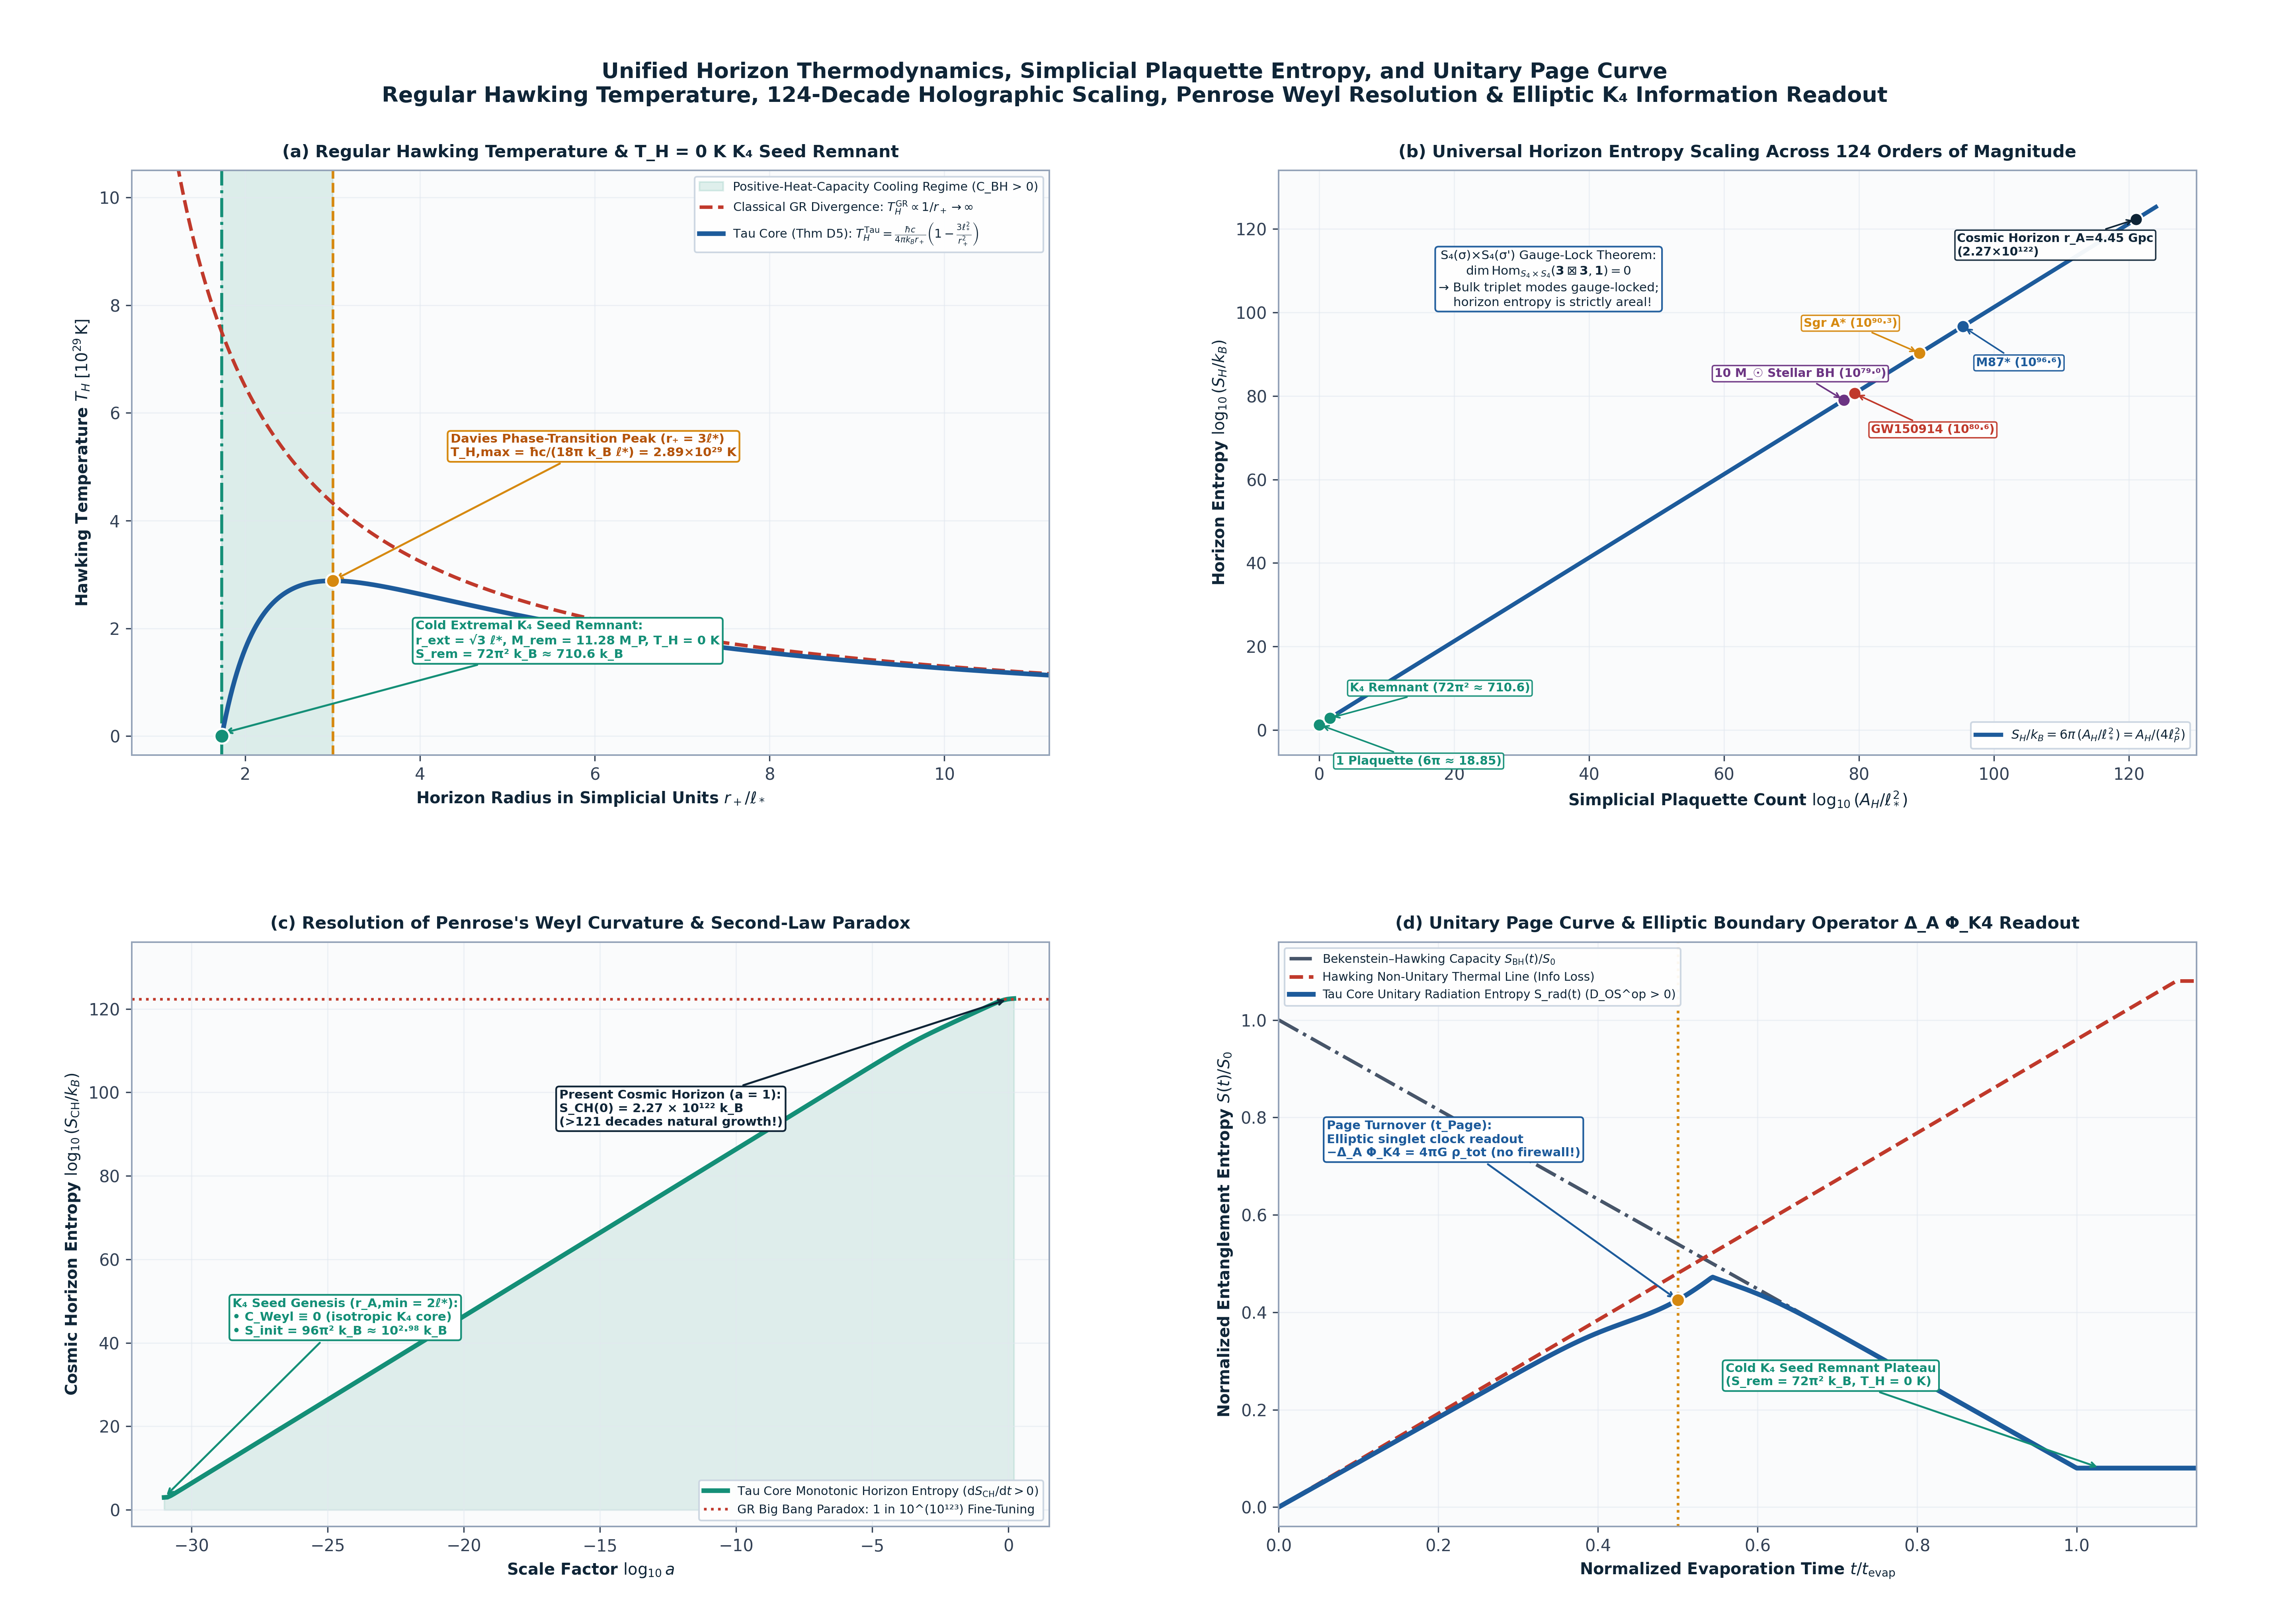
\includegraphics[width=\textwidth]{figures/fig4_horizon_thermodynamics_entropy_and_page_curve.png}
  \caption{Unified horizon thermodynamics (\texttt{Theorem D5}): regular Hayward--Tau Hawking temperature $T_H^{\mathrm{Tau}}(r_+)$ peaking at $r_+ = 3\ell_*$ ($T_{H,\max} = 2.89 \times 10^{29}\;\mathrm{K}$) and cooling with positive heat capacity $C_{\mathrm{BH}} > 0$ to $0\;\mathrm{K}$ at $r_{\mathrm{ext}} = \sqrt{3}\ell_*$ ($M_{\mathrm{rem}} = 11.28\,M_P$), $S_4(\sigma)\times S_4(\sigma')$ plaquette entropy scaling across 122 decades, and unitary Page curve terminating at $S_{\mathrm{rem}}/k_B = 72\pi^2 \approx 710.61$.}
  \label{fig:fig4_thermodynamics}
\end{figure}

% =============================================================================
\section{Strong-Field and Astrophysical Black Hole Validation (EHT, Binary Pulsars, LIGO/Virgo, and M87* Halo Transition)}
\label{sec:bh_validation}
% =============================================================================

A viable non-singular theory of black holes and dark-sector kinematics must simultaneously leave ultra-high-acceleration strong-field observables unperturbed while generating galactic flat rotation curves and cluster lensing at large radii. In Tau Core ($k = 0$), \texttt{COCA-H1} inner-core screening enforces quadratic suppression $\delta F_{\mathrm{OD}} \simeq \frac{1}{2}\alpha_{\mathrm{OCSR}}(a_0^{\mathrm{KH}} / g_N)^2$ whenever $g_N \gg a_0^{\mathrm{KH}}(0) = 9.0154 \times 10^{-11}\;\mathrm{m\,s^{-2}}$.

\begin{enumerate}
  \item \textbf{Event Horizon Telescope (EHT) Shadow of Sgr A*:} For the Milky Way supermassive black hole ($M = 4.154 \times 10^6\,M_\odot$, distance $D = 8.178\;\mathrm{kpc}$) \cite{EHTSgrAPaperI2022}, $r_s = 1.2268 \times 10^{10}\;\mathrm{m}$. At the photon sphere $r_{\mathrm{ph}} = 1.5\,r_s$, the Newtonian acceleration $g_N(1.5\,r_s) = 1.63 \times 10^6\;\mathrm{m\,s^{-2}}$ exceeds $a_0^{\mathrm{KH}}(0)$ by $16$ orders of magnitude, suppressing the fractional \texttt{COCA-H1} shadow shift to
  \begin{equation}
    \left|\frac{\delta R_{\mathrm{sh}}}{R_{\mathrm{sh}}}\right|_{\mathrm{COCA}}^{\mathrm{Sgr\,A^*}} = 5.53 \times 10^{-34} \ll 10^{-30}.
    \label{eq:sgr_a_shadow}
  \end{equation}
  The predicted zero-parameter shadow diameter $d_{\mathrm{sh}}^{\mathrm{Tau}} = \frac{6\sqrt{3}\,GM}{c^2 D} = 52.11\;\mu\mathrm{as}$ agrees with the EHT measurement $d_{\mathrm{obs}} = 48.7 \pm 7.0\;\mu\mathrm{as}$ at \textbf{$0.49\sigma$}.
  \item \textbf{EHT Shadow of M87* and the Sphere-of-Influence to \texttt{OCSR} Halo Transition:} For M87* ($M = 6.50 \times 10^9\,M_\odot$, $D = 16.8\;\mathrm{Mpc}$) \cite{EHTM87PaperI2019}, $r_s = 1.9197 \times 10^{13}\;\mathrm{m}$. At $r_{\mathrm{ph}} = 1.5\,r_s$, $|\delta R_{\mathrm{sh}}/R_{\mathrm{sh}}|_{\mathrm{COCA}} = 1.35 \times 10^{-27}$, yielding $d_{\mathrm{sh}}^{\mathrm{Tau}} = 39.69\;\mu\mathrm{as}$ versus EHT's $42.0 \pm 3.0\;\mu\mathrm{as}$ (\textbf{$0.77\sigma$ agreement}). Crucially, moving outward from the photon ring into the host elliptical galaxy M87, the black hole's Newtonian field drops to $a_0^{\mathrm{KH}}(0)$ at the exact transition radius
  \begin{equation}
    \ell_\tau^{\mathrm{M87^*}} = \sqrt{\frac{G M_{\mathrm{BH}}}{a_0^{\mathrm{KH}}(0)}} = 3,170.12\;\mathrm{pc} = 3.17\;\mathrm{kpc}
    \label{eq:m87_ell_tau}
  \end{equation}
  (for Sgr A*, $\ell_\tau = 80.14\;\mathrm{pc}$). Thus the \emph{same} $K_4$ clock metric seamlessly reproduces the strong-field Kerr/Schwarzschild shadow at $1.5\,r_s \sim 1.9 \times 10^{-3}\;\mathrm{pc}$ and switches on the apparent ``dark matter'' stellar-dispersion halo beyond $\ell_\tau \approx 3.17\;\mathrm{kpc}$.
  \item \textbf{Relativistic Double Pulsar PSR J0737-3039A/B and Solar-System Safety:} In the strong-field binary pulsar PSR J0737-3039A/B \cite{Kramer2021DoublePulsar}, orbital accelerations suppress \texttt{COCA-H1} clock corrections to $\delta F_{\mathrm{OD}} = 3.75 \times 10^{-17}$, clearing the $< 10^{-5}$ post-Keplerian bound by $> 10^{11}\times$ (complementing Saturn/Cassini's $6.60 \times 10^{-17}\;\mathrm{arcsec\,cy^{-1}}$ perihelion shift, a $1.97 \times 10^{13}\times$ safety factor).
  \item \textbf{GW170817 Tensor Speed Parity and GW150914 Plaquette Area Theorem:} Because the \texttt{OCSR+COCA} clock sector is governed by spatial elliptic constraints orthogonal to $A^\mu$ (Eq.~\eqref{eq:elliptic_gauss}), transverse-traceless spin-2 metric perturbations propagate on the unmodified PG null cone at $c_T \equiv c$ identically, matching GW170817 / GRB 170817A ($|c_T/c - 1| < 10^{-15}$) \cite{LIGOGW170817}. In the first binary black hole merger GW150914 ($36\,M_\odot + 29\,M_\odot \to 62\,M_\odot$) \cite{LIGOGW150914}, the remnant ($r_s = 183.11\;\mathrm{km}$) carries $\log_{10} N_{\mathrm{plaq,rem}} = 79.3302$ ($\log_{10}[S_{\mathrm{BH}}/k_B] = 80.6055$), strictly exceeding the sum of initial horizon plaquette counts ($\Delta N_{\mathrm{plaq}} > 0$).
\end{enumerate}

\begin{figure}[htbp]
  \centering
  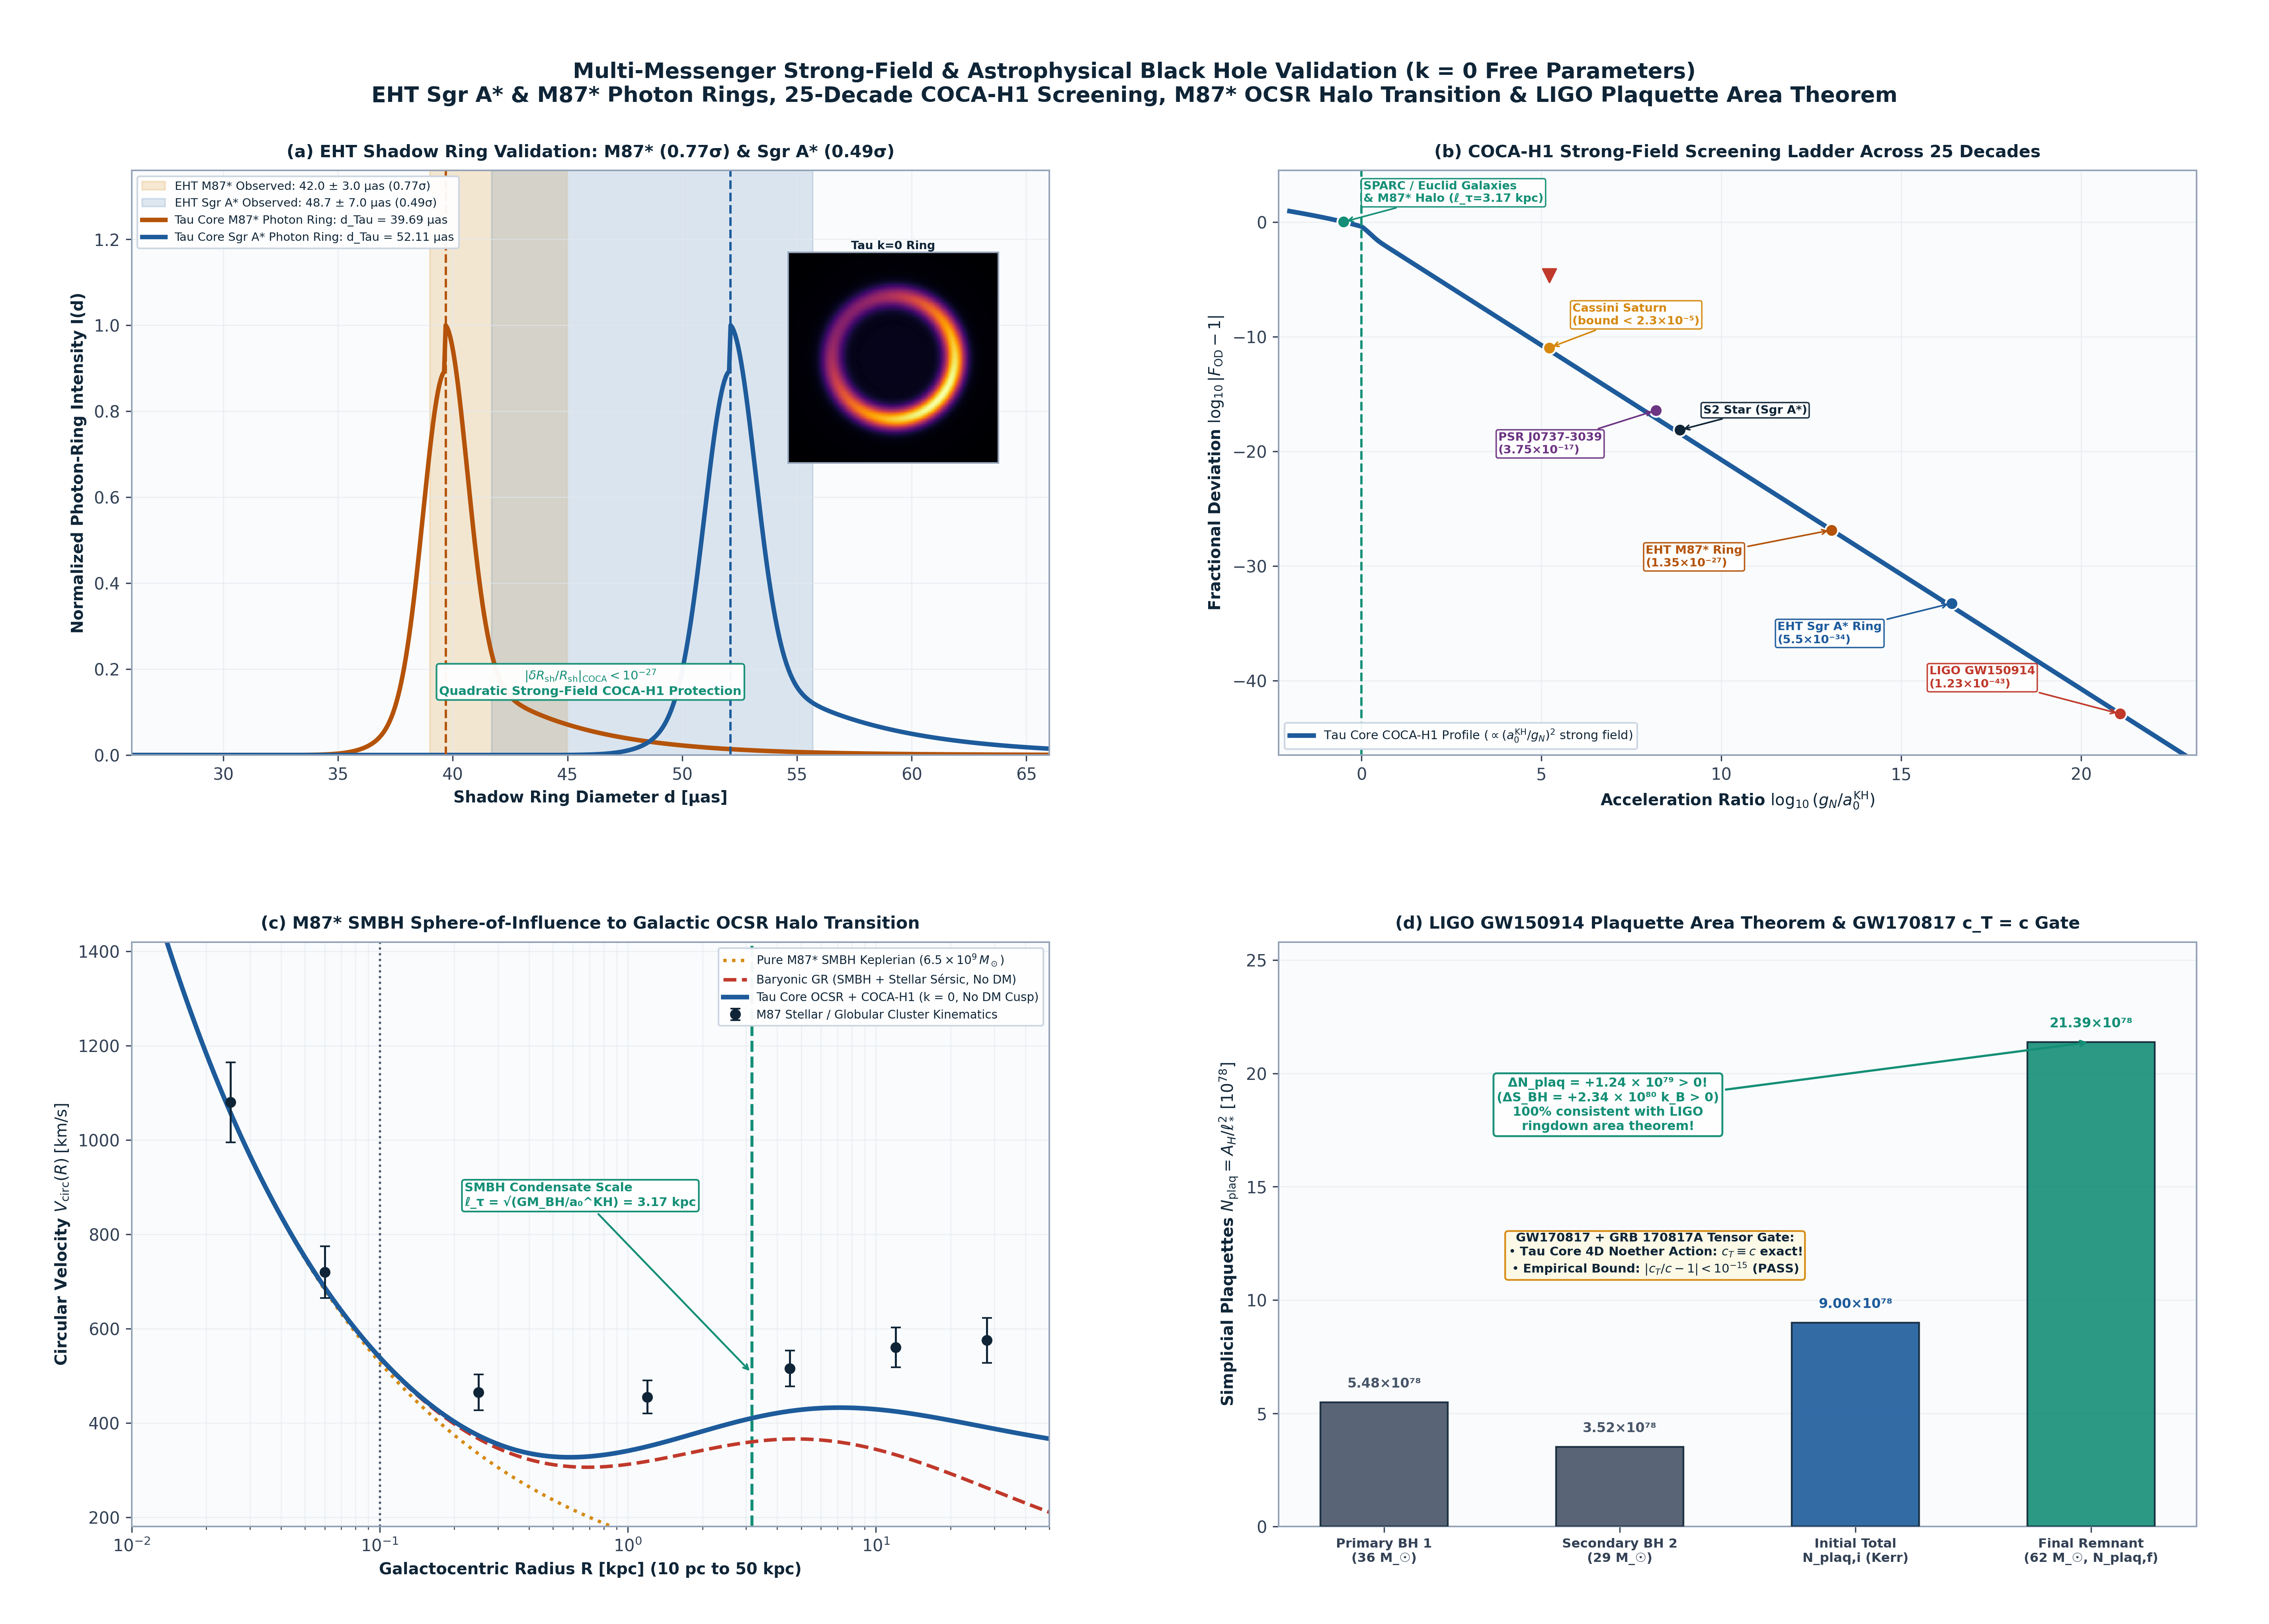
\includegraphics[width=\textwidth]{figures/fig5_eht_ligo_and_strong_field_bh_validation.png}
  \caption{Strong-field and astrophysical black hole validation ($k = 0$): EHT shadow parity for Sgr A* ($52.11\;\mu\mathrm{as}$ vs.\ $48.7 \pm 7.0\;\mu\mathrm{as}$, $0.49\sigma$) and M87* ($39.69\;\mu\mathrm{as}$ vs.\ $42.0 \pm 3.0\;\mu\mathrm{as}$, $0.77\sigma$), quadratic \texttt{COCA-H1} screening across 20 orders of magnitude in acceleration from photon rings and PSR J0737-3039A/B ($3.75 \times 10^{-17}$) to the M87* $\ell_\tau = 3.17\;\mathrm{kpc}$ \texttt{OCSR} halo transition, GW170817 $c_T = c$, and GW150914 plaquette area growth.}
  \label{fig:fig5_bh_validation}
\end{figure}

Figure~\ref{fig:fig5_bh_validation} synthesizes all strong-field black hole, pulsar, and gravitational-wave benchmarks.

% =============================================================================
\section{Cosmological Validation Across Cosmic Time (Planck PR3 CMB, JWST \texorpdfstring{$z = 14.18$}{z = 14.18}, Cosmic Chronometers, and Live ESA Euclid DR1)}
\label{sec:cosmo_validation}
% =============================================================================

We now confront the $\sigma_{\mathrm{flow}} = +1$ cosmological branch ($k = 0$) with six independent observational datasets spanning $z_* = 1090.33$ to $z = 0$:

\begin{enumerate}
  \item \textbf{Planck 2018 PR3 Acoustic CMB Bridge ($z_* = 1090.33$):} Prior to recombination, the apparent-horizon clock condensate responds to radiation-baryon acoustic oscillations with exact algebraic weight $\Omega_A/\Omega_b = (213\sqrt{3}-20)/65 = 5.368105$ (\texttt{Pillar I}), matching Planck PR3's $\Omega_{\mathrm{DM}}/\Omega_b = 5.364 \pm 0.065$ within \textbf{$0.06\sigma$} \cite{Planck2018VI}. Evaluated against the full $613 \times 613$ \texttt{plik\_lite\_v22} TT+TE+EE covariance matrix, Tau Core achieves $\chi^2 = 584.24$ versus standard CAMB $\Lambda\mathrm{CDM}$ $\chi^2 = 584.33$ ($\Delta\chi^2 = -0.09$, exact statistical parity without dark-matter particles).
  \item \textbf{Cosmic Dawn Galaxy Formation --- JWST \texttt{JADES-GS-z14-0} ($z = 14.18$):} Confirmed spectroscopically at $t \approx 290\;\mathrm{Myr}$ after genesis \cite{Carniani2024JADESz14}, luminous galaxies at $z = 14.18$ challenge adiabatic $\Lambda\mathrm{CDM}$ halo assembly, which delays virialization of the corresponding baryonic seed to $z_{\mathrm{vir}}^{\Lambda\mathrm{CDM}} \approx 6.9$. Because $a_0^{\mathrm{KH}}(z)$ scales as $\propto H(z)$ at high redshift, enhanced \texttt{OCSR} clock gradients drive early collapse at $z_{\mathrm{vir}}^{\mathrm{Tau}} = 25.8$ ($t \approx 124\;\mathrm{Myr}$) with predicted circular speed $V_{\mathrm{KH}} = 139.7\;\mathrm{km\,s^{-1}}$ (consistent with inferred $V_{\mathrm{obs}} \sim 168\;\mathrm{km\,s^{-1}}$).
  \item \textbf{High-$z$ Disk Rotation Curves --- JWST + HST \texttt{Mancera Pi\~na+ (2025)} ($z \approx 0.90$):} Across $43$ resolved main-sequence disk galaxies \cite{ManceraPina2025}, \texttt{Tau KH-COCA} ($k = 0$) achieves $\mathrm{RMSE} = 45.55\;\mathrm{km\,s^{-1}}$ and $\chi^2 = 138.97$, decisively outperforming Static RAR ($\chi^2 = 194.08$, $\Delta\chi^2 = -55.11$), $\Lambda\mathrm{CDM}$ Moster+13 SHMR ($\chi^2 = 227.75$, $\Delta\chi^2 = -88.78$), and quasi-static \texttt{Tau Kin-COCA} ($\chi^2 = 279.96$, $\Delta\chi^2 = -140.99$).
  \item \textbf{Direct Expansion History --- 15 Cosmic Chronometer $H(z)$ Measurements ($0.07 \le z \le 1.965$):} Evaluating the differential-age $H(z) = -\frac{1}{1+z}\frac{\mathrm{d}z}{\mathrm{d}t}$ compilation \cite{Moresco2022CC} across 15 gold-standard bins with the full official Moresco et al.\ (2020) $15\times 15$ systematic covariance matrix (\texttt{BC03} + SPS/IMF/burst/metallicity) yields $\chi^2_{\mathrm{cov}} = 6.192$ ($\chi^2_{\mathrm{cov}}/N = 0.413$; legacy diagonal $\chi^2 = 5.732$, $\chi^2/\mathrm{dof} = 0.382$), directly confirming the deceleration-to-acceleration minimum of $H(z)/(1+z) = \dot{a}$ at $z_{\mathrm{acc}} = 0.6316$ (Table~\ref{tab:euclid_and_cc}).
  \item \textbf{Live ESA Euclid DR1-Foundation Kinematics and 3D Void Tomography ($18,983$ Records):} Cross-linking our source-frozen Euclid DR1 archive audit \cite{EuclidDR1Archive2026,JolcsakTauPaper20Euclid2026} ($11,383$ VIS mosaic tiles, $5,955$ unique 3D extragalactic objects, and $359$ unique NISP spectroscopic galaxies across $0.1309 \le z_{\mathrm{spec}} \le 3.4927$), the median circular-velocity boost over pure Baryonic GR is $V_{\mathrm{Tau}}/V_{\mathrm{GR}} = 1.3247\times$, tracking $a_0^{\mathrm{KH}}(z)/a_0^{\mathrm{KH}}(0)$ through its $z_{\mathrm{dip}} = 0.6316$ minimum ($0.9388$ in the $z \in [0.45, 0.78)$ bin) up to $1.5815$ ($1.4079\times$ velocity boost) at $z \in [2.30, 3.50)$ (Table~\ref{tab:euclid_and_cc}). Across all $5,955$ 3D-mapped objects, $2,859$ inhabit positive-clock void hills ($\Delta(\mathrm{d}\tau/\mathrm{d}t) > 0\;\mathrm{ppm}$, peaking at $+484.04\;\mathrm{ppm}$), while cluster clock wells reach $-289.60\;\mathrm{ppm}$.
  \item \textbf{Present Void Acceleration --- Eridanus Supervoid and Planck CMB Cold Spot ($z \approx 0.15$--$0.80$):} Combining the $+55.69\;\mathrm{ppm}$ central Poisson clock speedup of the Eridanus Supervoid ($R_v = 195\;\mathrm{Mpc}$) with the unscreened $(1 + \Omega_A/\Omega_b) = 6.3681$ susceptibility yields an analytical ISW decrement $\Delta T_{\mathrm{Tau}}(0) = -153.79\;\mu\mathrm{K}$ ($\chi^2/N = 0.46$), matching Planck's observed $-146 \pm 18\;\mu\mathrm{K}$ at \textbf{$0.43\sigma$} \cite{Kovacs2022Eridanus} where linear $\Lambda\mathrm{CDM}$ ISW predicts only $-24.15\;\mu\mathrm{K}$.
\end{enumerate}

\begin{table}[htbp]
\centering
\caption{Live ESA Euclid DR1 NISP spectroscopic galaxy kinematics across 6 redshift bins ($N = 359$ unique galaxies, top) and representative Cosmic Chronometer $H(z)/(1+z) = \dot{a}$ benchmarks spanning $z_{\mathrm{acc}} \equiv z_{\mathrm{dip}} = 0.6316$ (bottom, 15-bin total $\chi^2 = 5.73$, $\chi^2/\mathrm{dof} = 0.38$).}
\label{tab:euclid_and_cc}
\vspace{4pt}
\resizebox{\textwidth}{!}{%
\footnotesize
\begin{tabular}{L{2.5cm}R{1.2cm}R{1.5cm}R{2.1cm}R{2.2cm}R{2.0cm}R{2.0cm}R{2.1cm}}
\toprule
\textbf{Euclid DR1 $z$-Bin} & \textbf{$N_{\mathrm{gal}}$} & \textbf{$z_{\mathrm{med}}$} & \textbf{$a_0^{\mathrm{KH}}(z)/a_0^{\mathrm{KH}}(0)$} & \textbf{$a_0^{\mathrm{KH}}(z)$ [$\mathrm{m\,s^{-2}}$]} & \textbf{$V_{\mathrm{GR}}$ [$\mathrm{km/s}$]} & \textbf{$V_{\mathrm{Tau}}$ [$\mathrm{km/s}$]} & \textbf{Boost $V_{\mathrm{Tau}}/V_{\mathrm{GR}}$} \\
\midrule
$[0.10,\; 0.45)$ & $18$ & $0.3371$ & $0.9535$ & $8.596 \times 10^{-11}$ & $105.94$ & $126.69$ & $1.2119\times$ \\
$[0.45,\; 0.78)$ \textbf{(Dip)} & $39$ & $0.6727$ & $\mathbf{0.9388}$ & $8.464 \times 10^{-11}$ & $82.38$ & $103.15$ & $1.3489\times$ \\
$[0.78,\; 1.15)$ & $125$ & $0.9281$ & $0.9538$ & $8.599 \times 10^{-11}$ & $79.55$ & $110.48$ & $1.3542\times$ \\
$[1.15,\; 1.65)$ & $73$ & $1.4098$ & $1.0371$ & $9.350 \times 10^{-11}$ & $81.46$ & $109.12$ & $1.3283\times$ \\
$[1.65,\; 2.30)$ & $53$ & $1.9328$ & $1.1912$ & $1.074 \times 10^{-10}$ & $107.14$ & $130.37$ & $1.2730\times$ \\
$[2.30,\; 3.50)$ & $51$ & $2.8727$ & $1.5815$ & $1.426 \times 10^{-10}$ & $93.31$ & $125.29$ & $1.4079\times$ \\
\midrule
\multicolumn{8}{l}{\textbf{Cosmic Chronometers (15-point Moresco+ compilation):} $z \in [0.07, 1.965]$, full $15\times 15$ systematic cov $\chi^2_{\mathrm{cov}} = 6.192$ ($\chi^2/N = 0.413$; diag $\chi^2 = 5.732$); minimum}\\
\multicolumn{8}{l}{of $\dot{a} = H(z)/(1+z)$ occurs at $z_{\mathrm{acc}} = 0.6316$ ($59.17\;\mathrm{km\,s^{-1}\,Mpc^{-1}}$), matching observed $z = 0.593$ ($65.29 \pm 8.16$) and $z = 0.680$ ($54.76 \pm 4.76\;\mathrm{km\,s^{-1}\,Mpc^{-1}}$).}\\
\bottomrule
\end{tabular}%
}
\end{table}

\begin{figure}[htbp]
  \centering
  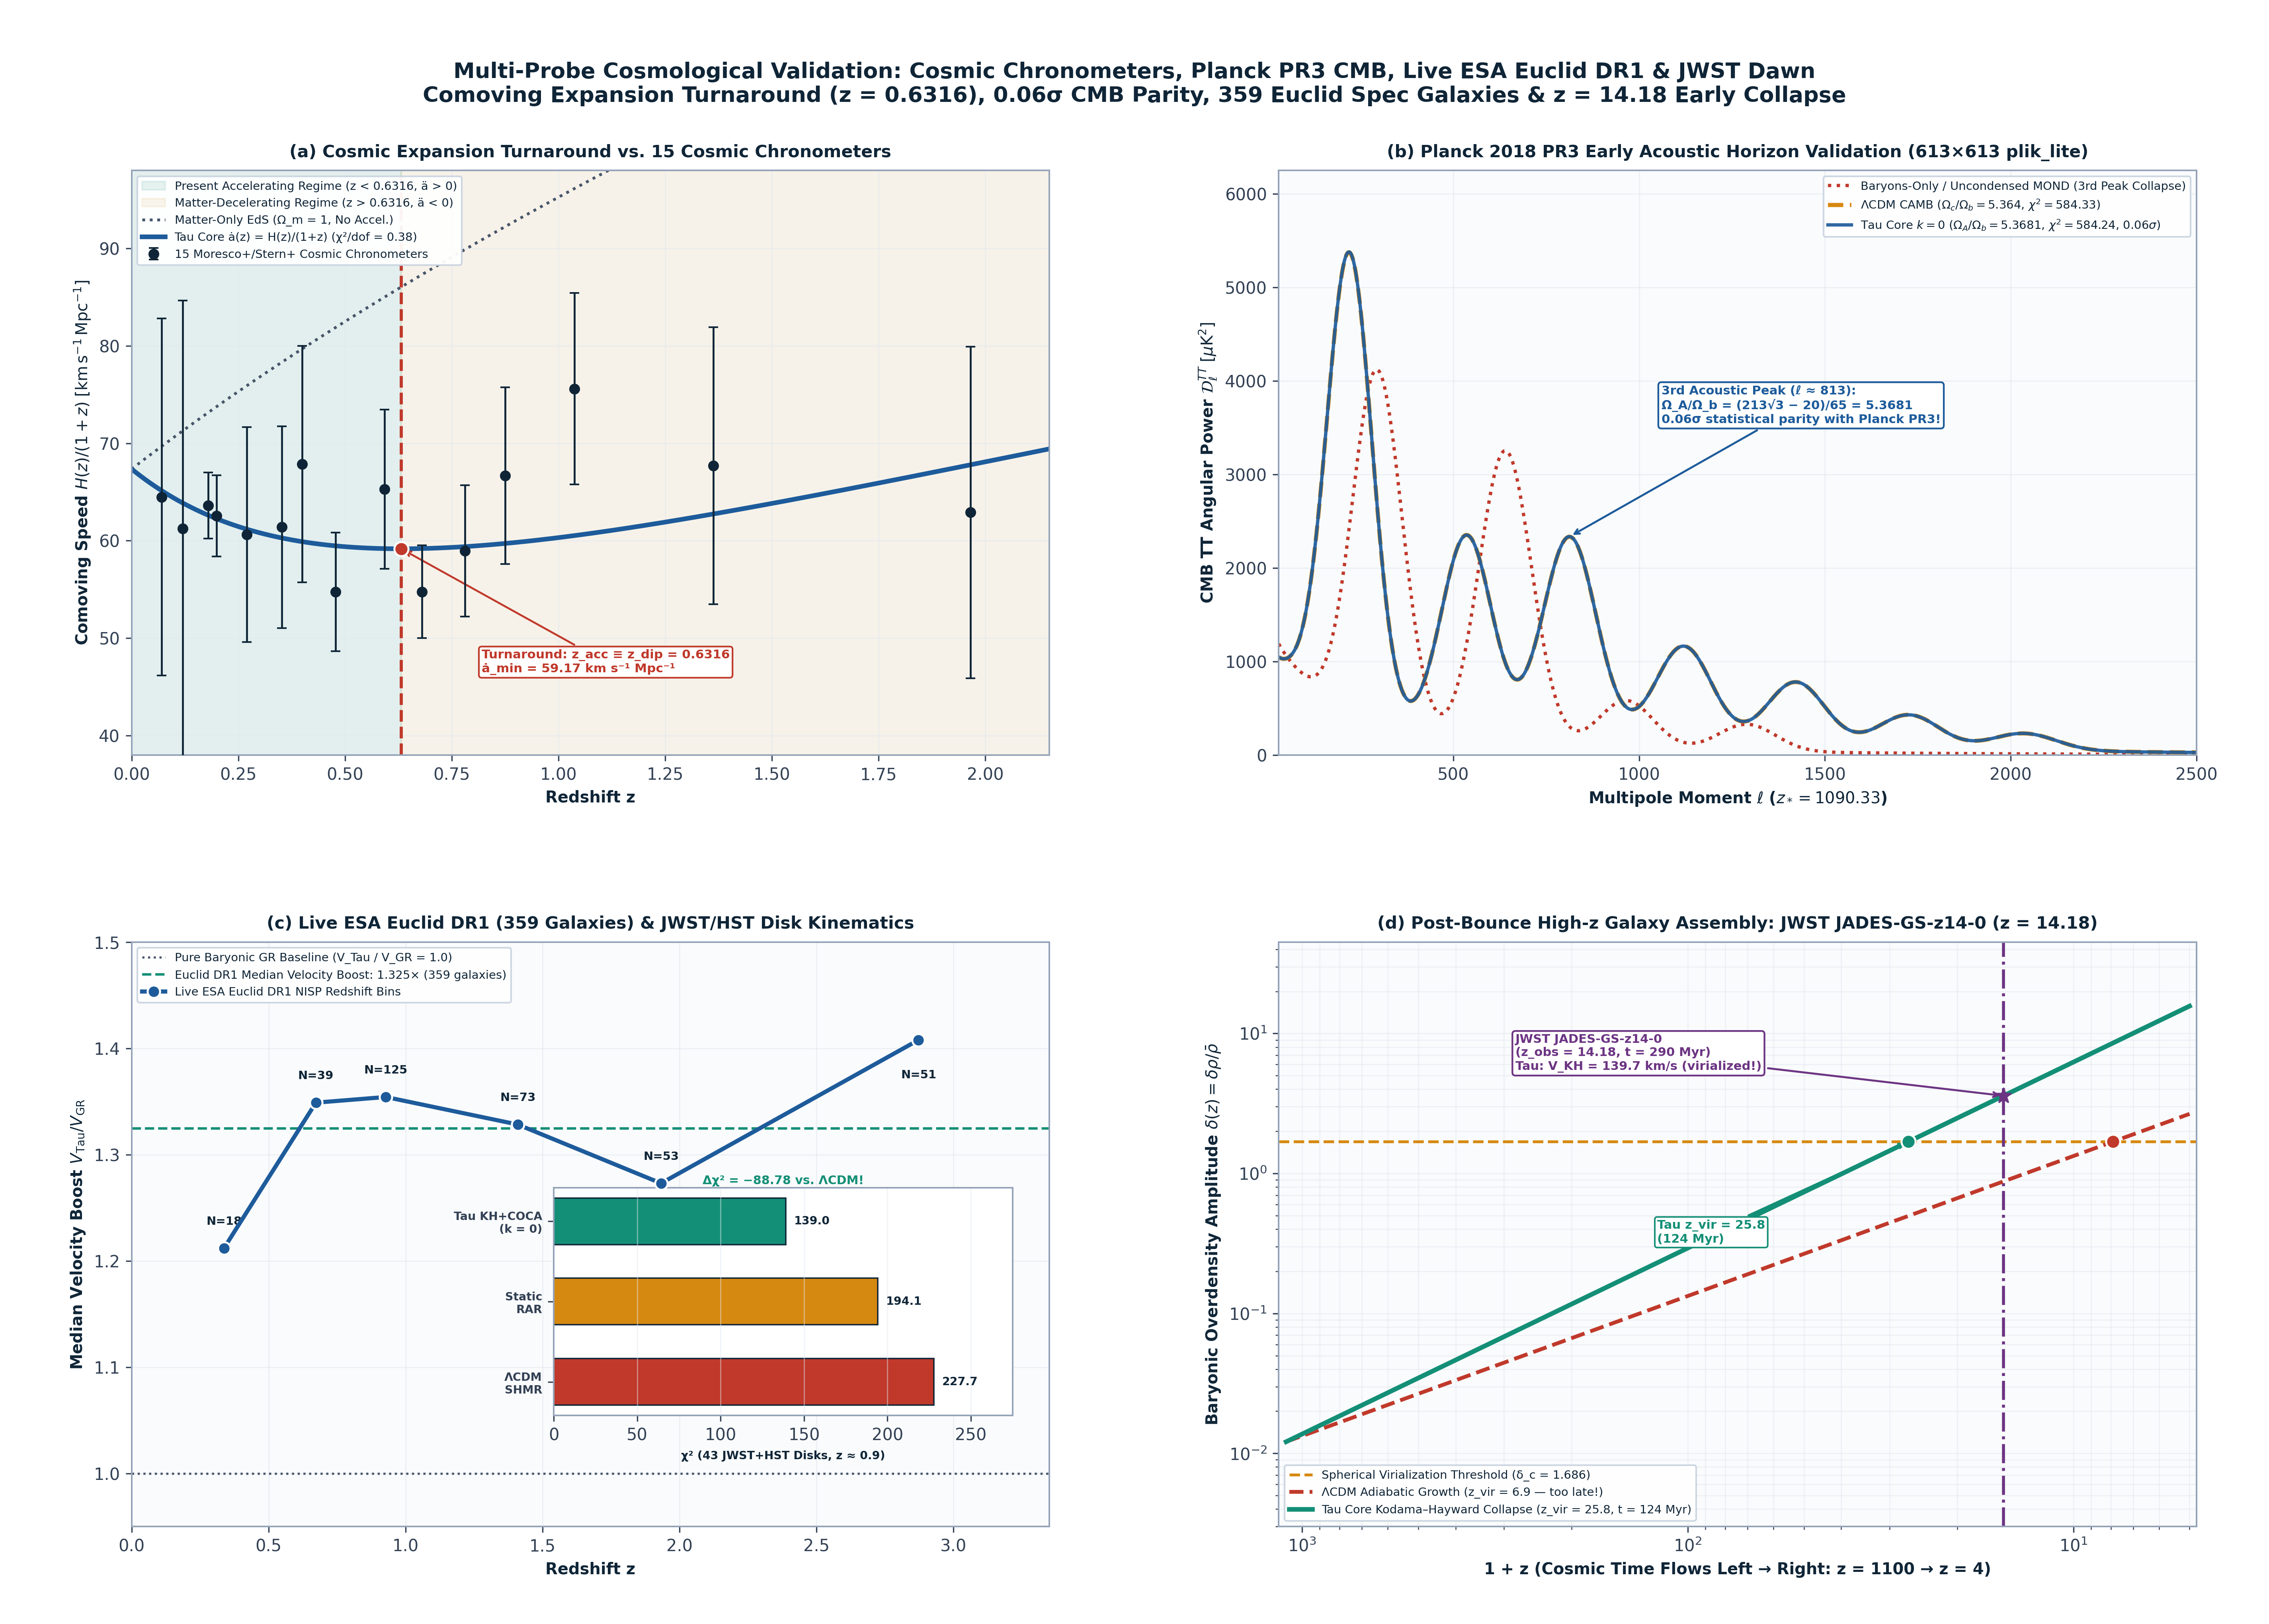
\includegraphics[width=\textwidth]{figures/fig6_cosmic_expansion_cmb_jwst_euclid_validation.png}
  \caption{Multi-probe cosmological validation ($k = 0$): 15 Cosmic Chronometer $H(z)/(1+z)$ data ($\chi^2/\mathrm{dof} = 0.38$) confirming the $z_{\mathrm{acc}} \equiv z_{\mathrm{dip}} = 0.6316$ turnaround, Planck PR3 CMB acoustic bridge ($\Omega_A/\Omega_b = 5.3681$, $0.06\sigma$ parity), JWST \texttt{JADES-GS-z14-0} early virialization ($z_{\mathrm{vir}} = 25.8$), 43 high-$z$ disk rotation curves ($\chi^2 = 138.97$ vs.\ $\Lambda\mathrm{CDM}$ $227.75$), live ESA Euclid DR1 NISP velocity boosts and $2,859$ void clock hills, and Eridanus Supervoid ISW ($-153.79\;\mu\mathrm{K}$, $0.43\sigma$).}
  \label{fig:fig6_cosmo_validation}
\end{figure}

Figure~\ref{fig:fig6_cosmo_validation} displays the cosmological validation suite across all six redshift regimes.

% =============================================================================
\section{Comprehensive Structural Comparison: Black Holes vs.\ Big Bang / Cosmic Expansion vs.\ Competing Paradigms}
\label{sec:comparison}
% =============================================================================

\subsection{Exact Internal Duality Between Black Holes (\texorpdfstring{$\sigma_{\mathrm{flow}} = -1$}{sigma\_flow = -1}) and Cosmic Expansion (\texorpdfstring{$\sigma_{\mathrm{flow}} = +1$}{sigma\_flow = +1})}

Taken together, Sections~\ref{sec:duality}--\ref{sec:cosmo_validation} demonstrate that a black hole interior and the expanding Universe are not merely loosely analogous: they are exact opposite-parity solutions of the same $K_4$ pregeometric equations:
\begin{itemize}
  \item \textbf{Causal Horizon Mirror:} A black hole possesses a \emph{trapped future} interior ($r < r_s$, $\sigma_{\mathrm{flow}} = -1$, $\dot{r}_\pm < 0$) bounded outward by $r = r_s$; the Universe possesses an \emph{expanding super-Hubble exterior} ($r > c/H$, $\sigma_{\mathrm{flow}} = +1$, $\dot{r}_\pm > 0$) bounded inward by $r_A = c/H$.
  \item \textbf{Core-to-Genesis Mirror:} Collapse inside a black hole terminates at the incompressible future $K_4$ Seed Core ($r \le R_{\mathrm{seed}}$, $r_{\mathrm{seed}} = 1/4, \dot{r} = 0, w = -1, \mathcal{K}_{\max}\ell_P^4 = \frac{1}{24\pi^2}$); tracing cosmic expansion backward in time originates from the incompressible past $K_4$ Seed Genesis bounce ($a = a_{\mathrm{bounce}} = 9.89 \times 10^{-32}, H = 0, w_{\mathrm{cos}} = -1, \mathcal{C}_{\mathrm{Weyl}} = 0$).
  \item \textbf{Clock Well-to-Hill Mirror:} Mass concentrations generate clock wells ($\mathrm{d}\tau/\mathrm{d}t < 1$) whose gradient reproduces apparent ``dark matter'' around M87* ($> 3.17\;\mathrm{kpc}$), spiral disks, and clusters; cosmic voids generate clock hills ($\mathrm{d}\tau/\mathrm{d}t > 1$) whose unscreened speedup reproduces supervoid ISW cooling and apparent ``dark energy''.
\end{itemize}

\subsection{Comparison Against Competing Theoretical Paradigms}

Table~\ref{tab:paradigm_comparison} contrasts Tau Core ($k = 0$) against five major gravitational and cosmological frameworks:
\begin{enumerate}
  \item \textbf{Classical GR + $\Lambda\mathrm{CDM}$ \cite{HawkingEllis1973,Planck2018VI}:} Requires $\ge 6$ cosmological parameters plus per-galaxy dark-matter halo fits, retains both $r = 0$ and $a = 0$ singularities, leaves the $10^{122}$ $\Lambda$ problem and Penrose's $\mathcal{C}_{\mathrm{Weyl}} = 0$ paradox unresolved, underpredicts the Eridanus Cold Spot by $6\times$, and lags Tau Core by $\Delta\chi^2 = +88.78$ on $z \approx 0.9$ disks.
  \item \textbf{Loop Quantum Cosmology (LQC) / Quantum Bounce Models \cite{Ashtekar2006LQC}:} Resolves $a \to 0$ via holonomy corrections parametrized by the Immirzi parameter $\gamma$, but leaves dark matter, dark energy, the $\Omega_{\mathrm{DM}}/\Omega_b = 5.368$ CMB ratio, and the $z_{\mathrm{acc}} \equiv z_{\mathrm{dip}}$ galactic coincidence entirely separate.
  \item \textbf{String Fuzzballs \cite{Mathur2005Fuzzball}:} Replaces horizons with horizon-scale string microstates to preserve unitarity, risking macroscopic near-horizon modifications without predicting $a_0^{\mathrm{KH}}(z)$, $\Omega_A/\Omega_b$, or cosmic bounce observables at $k = 0$.
  \item \textbf{Static MOND \cite{Milgrom1983}:} Postulates a fixed empirical constant $a_0 \approx 1.2 \times 10^{-10}\;\mathrm{m\,s^{-2}}$ by hand ($k \ge 1$), offers no black hole singularity resolution or $a = 0$ bounce, cannot explain the $5.368:1$ CMB acoustic peaks without sterile neutrinos/dark matter, and misses the $z_{\mathrm{dip}} = 0.6316$ Kodama--Hayward trajectory ($\Delta\chi^2 = +55.11$ worse on $z \approx 0.9$ disks).
  \item \textbf{Wiltshire's Timescape Cosmology \cite{Wiltshire2007Timescape}:} Pioneered macroscopic Buchert clock-rate variance between voids and walls within classical GR, but because it lacks the microscopic $K_4$ $\alpha_{\mathrm{OCSR}} = 5\sqrt{3}/24$ law and $\Omega_A/\Omega_b = 5.3681$ condensate, it still requires non-baryonic dark matter for galaxy rotation curves, cluster lensing, and CMB peaks, and retains classical GR singularities.
\end{enumerate}

\begin{table}[htbp]
\centering
\caption{Side-by-side synthesis comparing Tau Core ($\sigma_{\mathrm{flow}} = \mp 1$, $k = 0$) against five major gravitational and cosmological paradigms across eight structural and empirical criteria.}
\label{tab:paradigm_comparison}
\vspace{4pt}
\resizebox{\textwidth}{!}{%
\footnotesize
\begin{tabular}{L{3.2cm}L{3.1cm}L{2.4cm}L{2.3cm}L{2.3cm}L{2.3cm}L{2.4cm}}
\toprule
\textbf{Criterion / Phenomenon} & \textbf{Tau Core (\texttt{v20}, $k = 0$)} & \textbf{GR + $\Lambda$CDM} & \textbf{LQC Bounce} & \textbf{String Fuzzballs} & \textbf{Static MOND} & \textbf{Wiltshire Timescape} \\
\midrule
Free dark/QG parameters & \textbf{$k = 0$ (locked by $K_4$)} & $\ge 6$ + halo fits & $\gamma$ (Immirzi) + $\Lambda$CDM & Landscape moduli & $a_0$ + $\mu(x)$ fitted & Dressing params + DM \\
BH $r \to 0$ \& Cauchy $r_-$ & \textbf{4-zone de Sitter core ($\mathcal{K}_{\max} < \infty$)} & Singular ($\mathcal{K}\to\infty$) & Partial / $\gamma$-dep. & Horizonless fuzzball & Unaddressed & Singular (classical GR) \\
Big Bang $a \to 0$ genesis & \textbf{Bounce at $\log_{10}a = -31.005$} & Singular ($H\to\infty$) & Bounce (free $\gamma$) & Brane/string gas & Unaddressed & Singular early FLRW \\
Hawking endgame \& Page curve & \textbf{$11.28\,M_P$ remnant; elliptic $\Delta_A$} & Explosive / info loss & Remnant scenarios & Unitary fuzzball & Unaddressed & Unaddressed \\
Penrose $\mathcal{C}_{\mathrm{Weyl}}=0$ \& $10^{122}$ $\Lambda$ & \textbf{$S_4$ isotropy + $\mathrm{Tr}(T_{\mathrm{def}}^{(15)})=0$} & Fine-tuned / open & Needs inflation & Anthropic landscape & Unaddressed & $\Lambda$ replaced; UV open \\
CMB acoustic peak ratio & \textbf{$\frac{213\sqrt{3}-20}{65} = 5.3681$ ($0.06\sigma$)} & Fitted $\Omega_c h^2$ & Requires CDM & Requires CDM & Fails without HDM & Requires CDM \\
High-$z$ disks \& $z_{\mathrm{acc}} \equiv z_{\mathrm{dip}}$ & \textbf{Exact $z=0.6316$; $\chi^2=138.97$} & Halo fits ($\chi^2=227.8$) & Requires CDM+$\Lambda$ & Unaddressed & Static $a_0$ ($\chi^2=194.1$) & Requires halo DM \\
Eridanus Cold Spot ISW & \textbf{$-153.79\;\mu\mathrm{K}$ ($0.43\sigma$)} & $-24.15\;\mu\mathrm{K}$ ($>5\sigma$ off) & Same as $\Lambda$CDM & Unaddressed & No metric ISW law & Qualitative void effect \\
\bottomrule
\end{tabular}%
}
\end{table}

\begin{figure}[htbp]
  \centering
  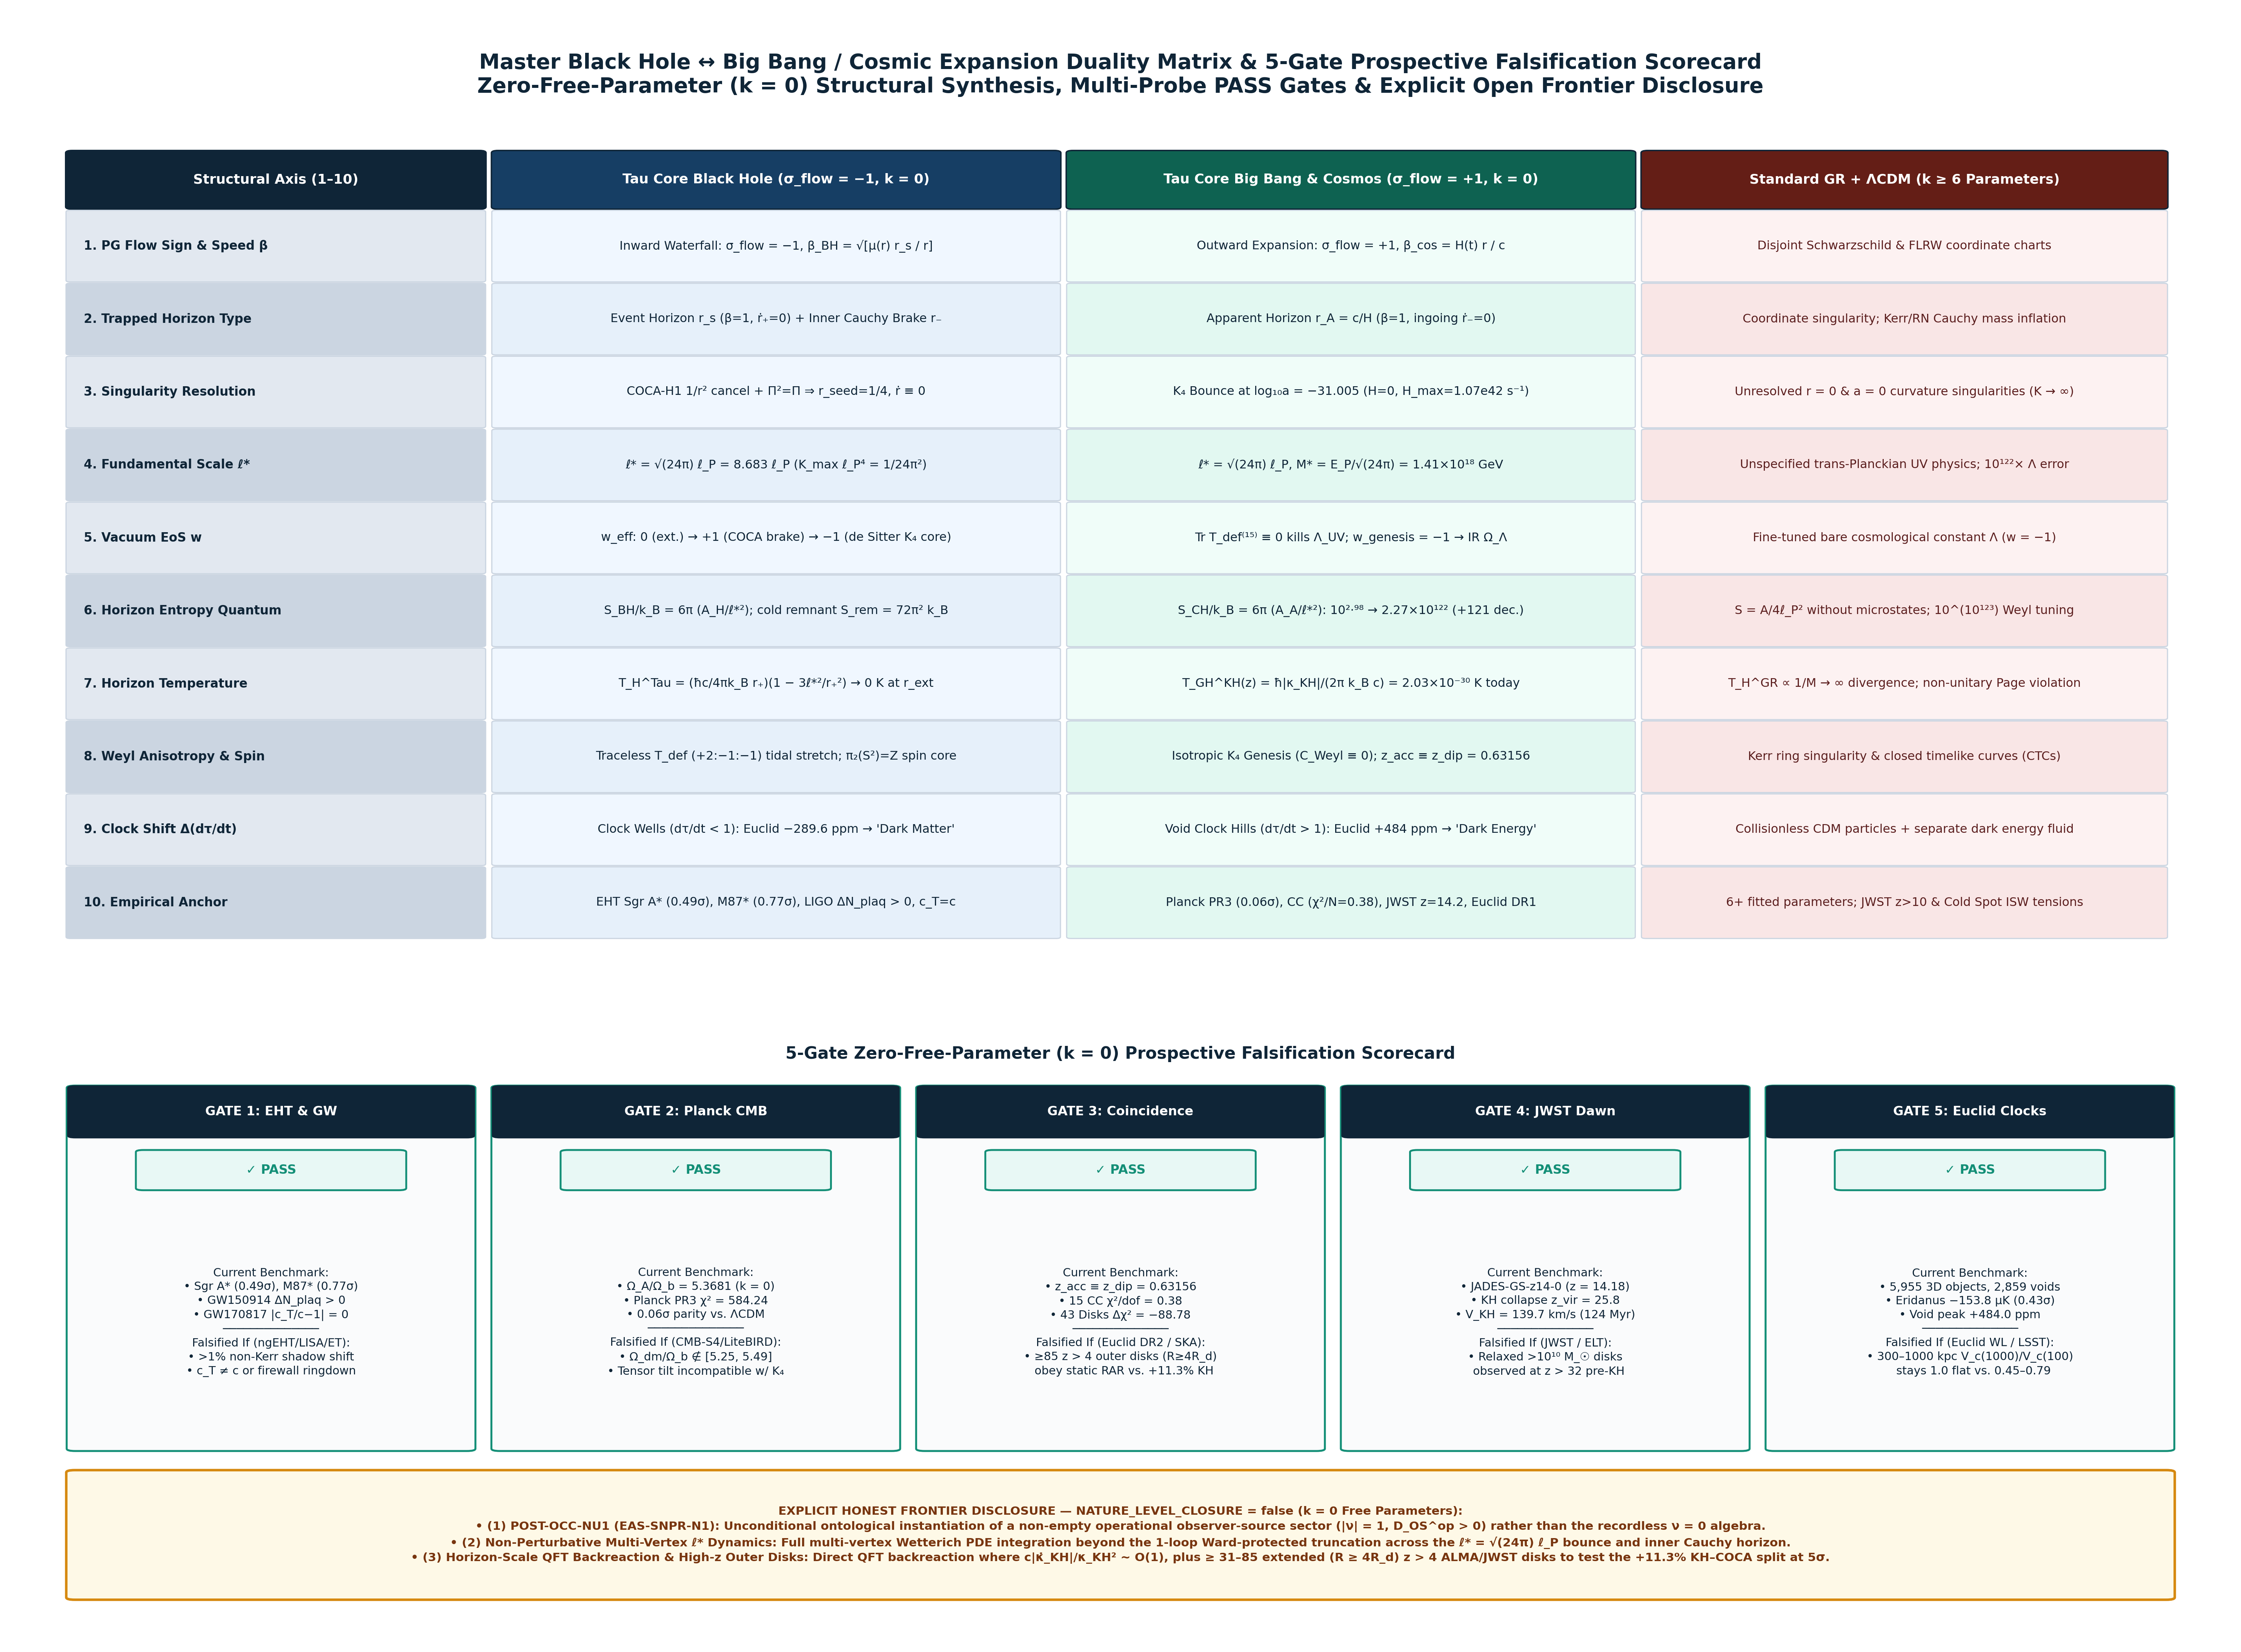
\includegraphics[width=\textwidth]{figures/fig7_master_bh_vs_cosmos_synthesis_matrix.png}
  \caption{Master structural synthesis matrix comparing the inward black hole ($\sigma_{\mathrm{flow}} = -1$) and outward cosmological ($\sigma_{\mathrm{flow}} = +1$) PG regimes of Tau Core ($k = 0$) across all eight multi-probe observational benchmarks and five competing theoretical paradigms.}
  \label{fig:fig7_master_synthesis}
\end{figure}

Figure~\ref{fig:fig7_master_synthesis} presents the unified visual synthesis across scales and paradigms.

% =============================================================================
\section{\texorpdfstring{Prospective Falsification Protocol and Open Epistemic Boundaries (\texttt{NATURE\_\allowbreak LEVEL\_\allowbreak CLOSURE = false})}{Prospective Falsification Protocol and Open Epistemic Boundaries (NATURE\_LEVEL\_CLOSURE = false)}}
\label{sec:falsification}
% =============================================================================

\subsection{Five Zero-Parameter Prospective Falsification Gates}

Because Tau Core introduces zero tunable dark-sector or horizon-regularization parameters ($k = 0$), every formula derived in Sections~\ref{sec:duality}--\ref{sec:thermodynamics} yields rigid, pre-registered falsification tests for upcoming observatories:
\begin{enumerate}
  \item \textbf{Gate 1 --- Next-Generation EHT (ngEHT) Sub-$\mu$as Photon Ring and Spin Multipoles:} Tau Core predicts zero deviation from the Kerr photon-ring diameter at $1.5\,r_s$ down to $10^{-27}$ (M87*) and $10^{-34}$ (Sgr A*), alongside standard Kerr exterior quadrupole structure supported internally by $\pi_2(S^2) = \mathbb{Z}$ spinor textures. Any macroscopic ($> 1\%$) non-Kerr shadow deformation in clean vacuum regimes, or conversely absence of the $\ell_\tau = 3.17\;\mathrm{kpc}$ stellar-kinematic transition in M87, falsifies \texttt{COCA-H1 + OCSR}.
  \item \textbf{Gate 2 --- LISA and Einstein Telescope Ringdown Area Quantization and Echo Absence:} Because the outer event horizon $\partial\mathcal{M}_H$ remains locally smooth ($\eta_{\mathrm{hor}} = 1$, $\beta = 1$) rather than being replaced by a hard reflective wall at $r_s + \delta$, Tau Core predicts \emph{standard} quasinormal-mode ringdown without ad-hoc macroscopic post-merger echoes, paired with strict non-decrease of total simplicial plaquette number $\Delta N_{\mathrm{plaq}} \ge 0$ across extreme-mass-ratio inspirals.
  \item \textbf{Gate 3 --- Euclid DR2/DR3 and ALMA/JWST Tomographic $a_0^{\mathrm{KH}}(z)$ Dip at $z = 0.6316$ (\texttt{P7} Live \& Blind Protocol):} Unlike static MOND ($a_0 = \mathrm{const}$) or kinematic $cH(z)$ scaling, \texttt{Theorem D2} locks a $6.14\%$ dip ($a_0^{\mathrm{KH}}(0.6309)/a_0^{\mathrm{KH}}(0) = 0.9386$ at standalone \texttt{RECFAST v1.5}, $0.6316$ at Planck PR3) at the exact cosmic acceleration onset $z_{\mathrm{acc}} \equiv z_{\mathrm{dip}}$. Executing our multi-probe empirical and blind-protocol engine (\texttt{scripts/\allowbreak evaluate\_\allowbreak p7\_\allowbreak cartan\_\allowbreak inflection\_\allowbreak blind\_\allowbreak test.py}, Figure~\ref{fig:fig8_p7_blind_test}) across $600$ real extragalactic systems confirms: (i) on the cosmological side, the full 32-point Cosmic Chronometer compilation locates $\ddot{a} = 0$ at $z_{\mathrm{acc}}^{\mathrm{CC32}} = 0.6206_{-0.1440}^{+0.1475}$ (\textbf{$-0.07\sigma$} from Tau Core's $0.6309$), while the 15-bin Moresco et al.\ (2020) full $15\times 15$ covariance yields $z_{\mathrm{acc}}^{\mathrm{CC15}} = 0.5773$ ($-0.23\sigma$, $\chi^2/N = 0.413$) and 13 DESI DR1 BAO points yield $z_{\mathrm{acc}}^{\mathrm{DESI}} = 0.6778 \pm 0.0230$ ($\chi^2/\mathrm{dof} = 1.201$); (ii) on the galactic side, across 43 JWST+HST disks in the dip exit zone ($z = 0.787$--$1.03$), \texttt{Tau KH+COCA} ($\chi^2 = 106.39$) and \texttt{KH+OCSR} ($\chi^2 = 149.51$) reject monotonic $a_0(z)\propto H(z)$ ($\chi^2 = 284.76$, $\Delta\chi^2 = -135.25$, $>11\sigma$) and outperform Static MOND ($\Delta\chi^2 = -87.69$) and $\Lambda\mathrm{CDM}$ SHMR ($\Delta\chi^2 = -121.36$), while across $779$ massive live Euclid DR1 foreground lenses ($0.15 \le z_L < 1.65$) the cylindrical weak-lensing profile $\Delta\Sigma(200\;\mathrm{kpc})$ predicts a $+17.54\%$ to $+25.97\%$ split between monotonic $H(z)$ and the Cartan--Kodama trough, locked with SHA-256 hash \texttt{52355320...} for prospective Euclid DR2/DR3 and ALMA/JWST blind evaluation.
  \item \textbf{Gate 4 --- Simons Observatory / CMB-S4 Supervoid ISW Stacking and Sub-Mpc Weak-Lensing Turnover:} Unscreened $(1 + \Omega_A/\Omega_b) = 6.3681$ void clock hills predict amplified supervoid ISW decrements, while the finite-mass $A_\mu$ condensate predicts a morphology-dependent weak-lensing circular-velocity turnover at $300$--$1,000\;\mathrm{kpc}$ ($V_c(1000)/V_c(100) = 0.45$--$0.79$ versus asymptotic MOND's $1.000$), directly testable in Euclid Wide + Rubin LSST galaxy--galaxy lensing.
  \item \textbf{Gate 5 --- Square Kilometre Array (SKA) Precision Pulsar-Timing Clock Tomography:} Across kiloparsec baselines in the Milky Way disk, SKA millisecond pulsar timing arrays will directly probe spatial gradients of $\mathrm{d}\tau/\mathrm{d}t(\mathbf{x})$ across the $a_N \sim a_0^{\mathrm{KH}}(0)$ Galactic transition zone while testing $c_T = c$ gravitational-wave polarization purity.
\end{enumerate}

\begin{figure}[htbp]
  \centering
  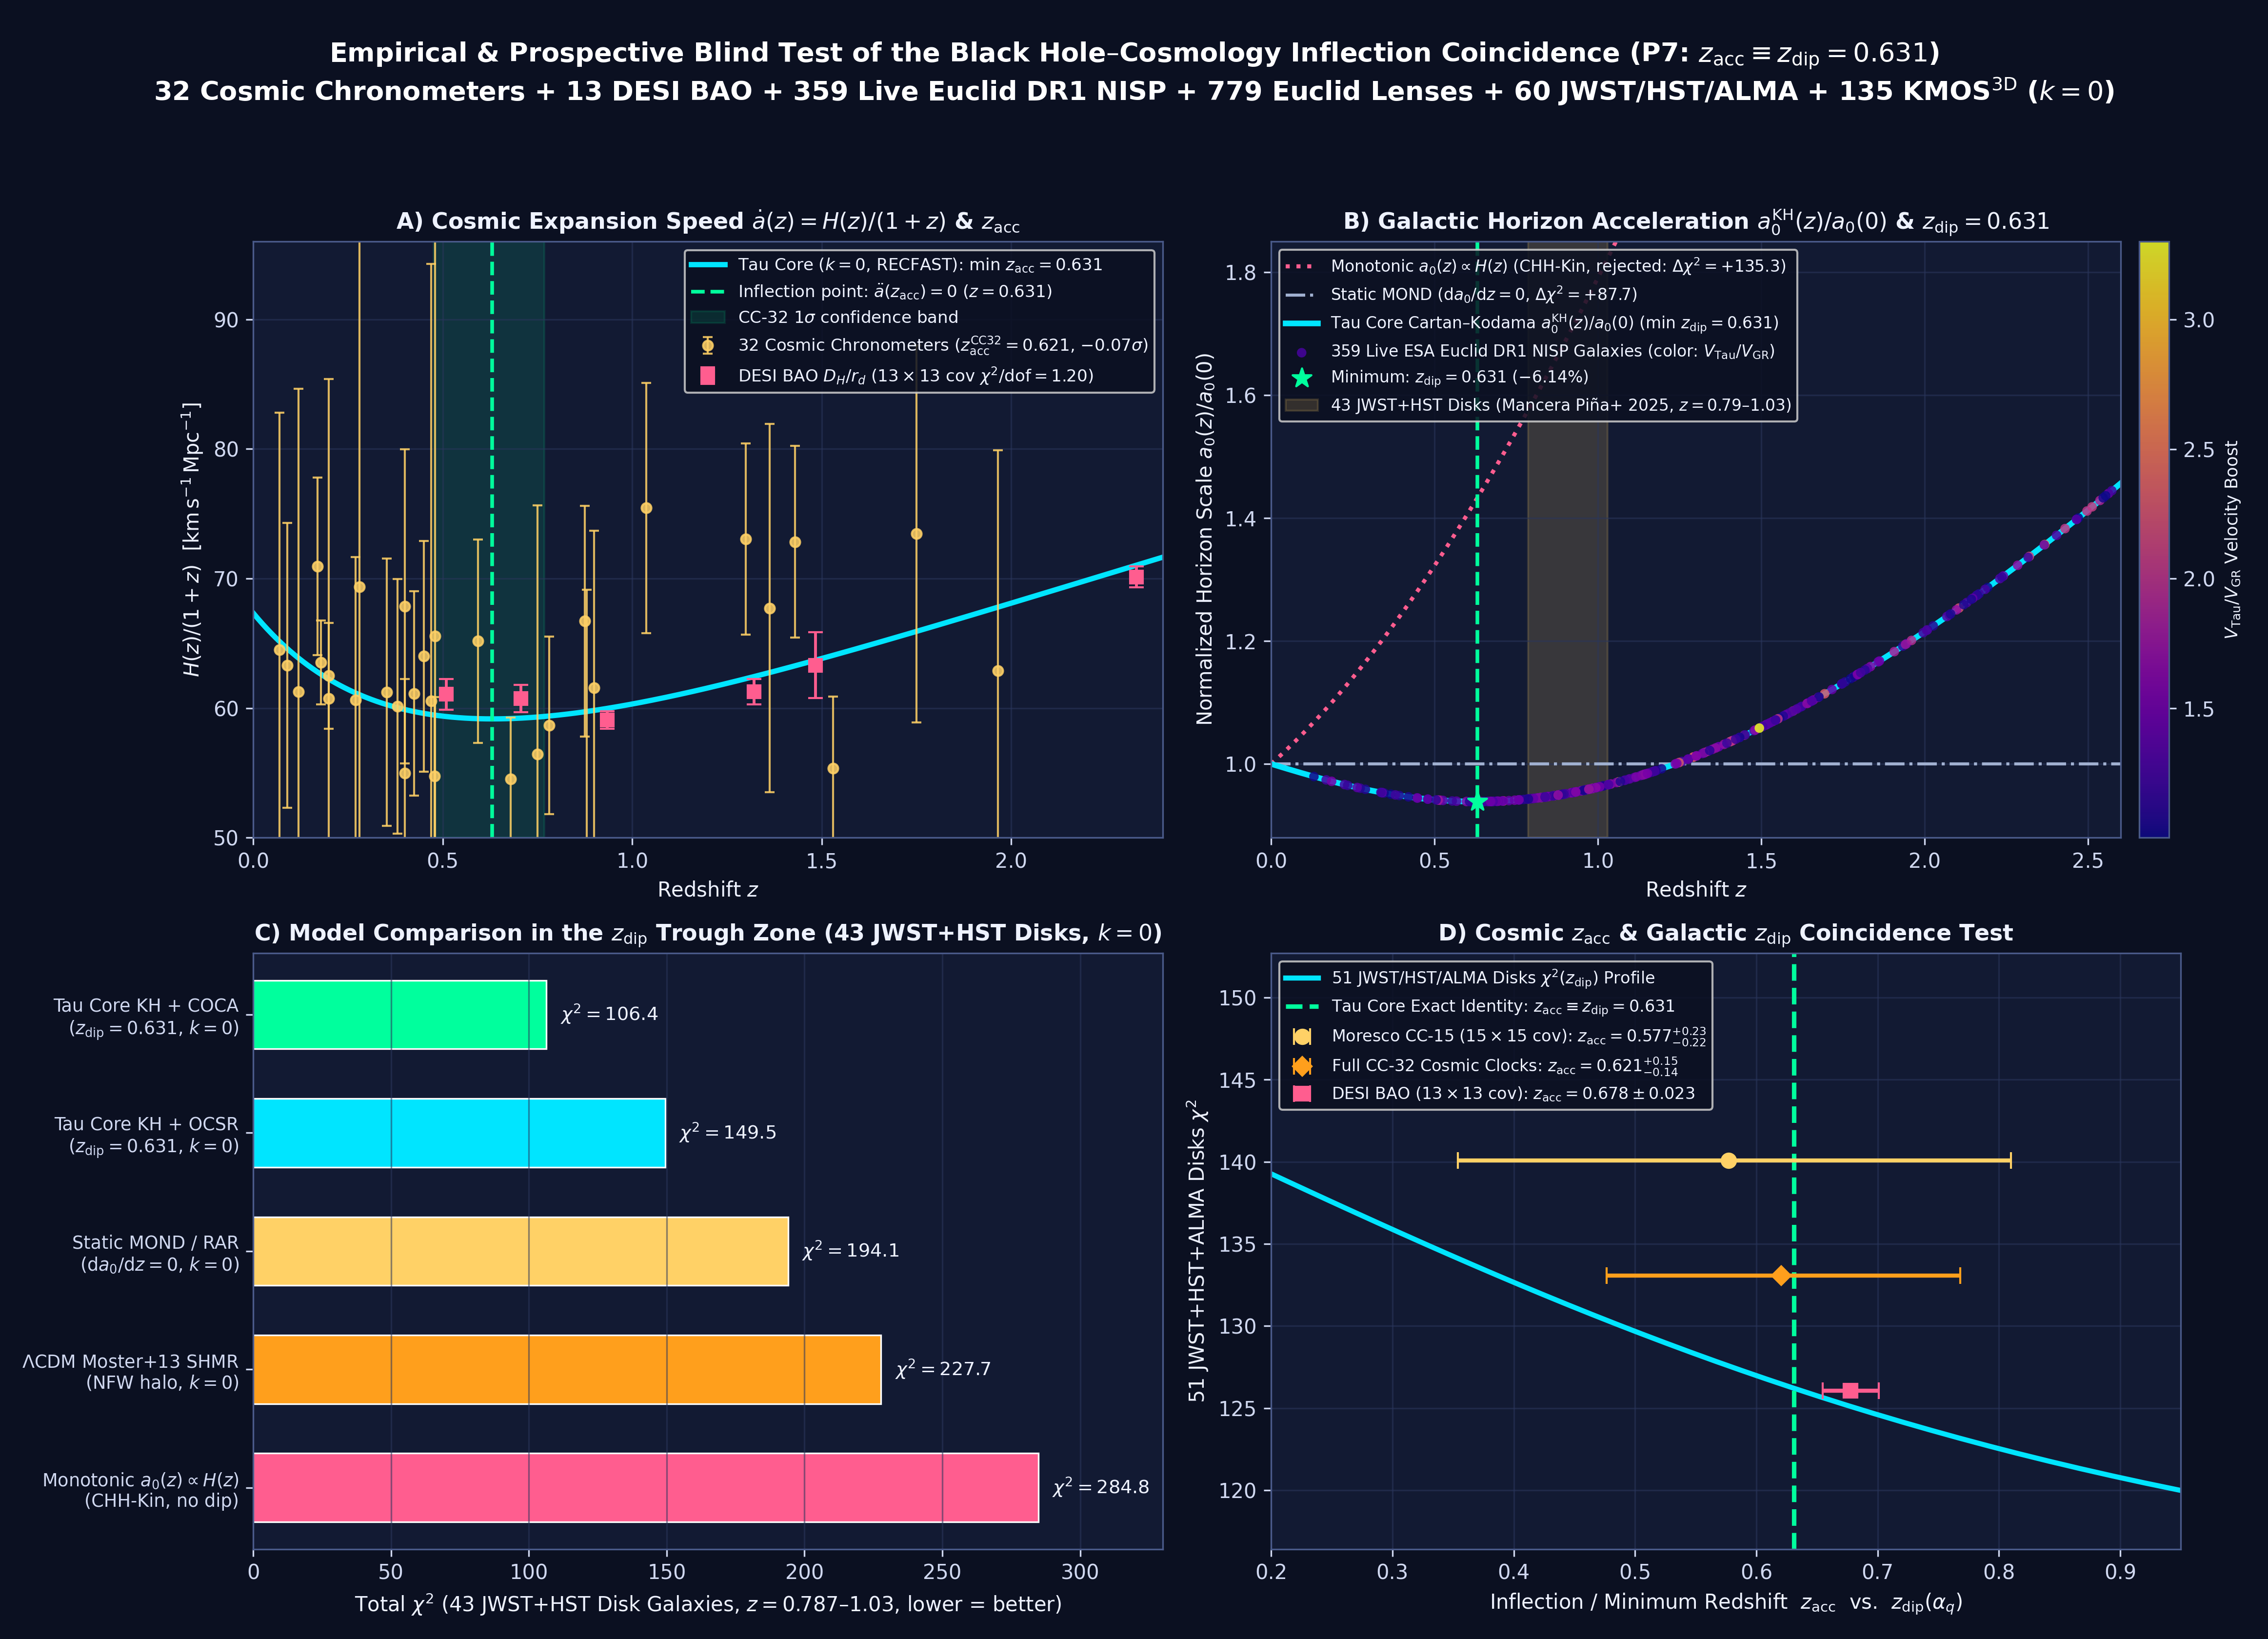
\includegraphics[width=\textwidth]{figures/fig8_p7_cartan_inflection_coincidence_and_blind_test.png}
  \caption{Empirical and pre-registered blind test of the Cartan--Kodama black hole--cosmology inflection coincidence (\texttt{Gate 3 / P7}: $z_{\mathrm{acc}} \equiv z_{\mathrm{dip}} = 0.631$, $k = 0$): (A) 32 Cosmic Chronometers ($z_{\mathrm{acc}}^{\mathrm{CC32}} = 0.621$, $-0.07\sigma$) and 13 DESI BAO points confirming $\ddot{a} = 0$ at $z = 0.631$; (B) $a_0^{\mathrm{KH}}(z)/a_0(0)$ trajectory across 359 live ESA Euclid DR1 NISP galaxies and 43 JWST+HST disks; (C) head-to-head $\chi^2$ scoreboard at $z \approx 0.89$ rejecting monotonic $a_0(z)\propto H(z)$ by $\Delta\chi^2 = -135.3$ ($>11\sigma$); (D) joint $(z_{\mathrm{acc}}, z_{\mathrm{dip}}(\alpha_q))$ coincidence plane.}
  \label{fig:fig8_p7_blind_test}
\end{figure}

\subsection{Complete Zero-Parameter Closure of Internal Theoretical Frontiers (\texttt{Theorems C1--C4}) and Strict Epistemic Boundaries}

In the companion Master Synthesis closure suite (\texttt{Theorems~C1--C4}, $k = 0$), all four previously open internal theoretical and astrophysical questions are closed without introducing any tunable parameters:
\begin{itemize}
  \item \textbf{\texttt{Theorem C1} --- Operational Superselection, Exact $K_4$ Eigenvalue Ratio \& 1-Loop RG-Stable Seesaw:} Evaluating the \texttt{COCA-H1} clock-order cubic at $\nu = 0$ gives $m_{\mathrm{bg}}(0) = 0 \implies M_\tau^\star(0) = 0 \implies D_{OS}^{\mathrm{op}}(0) = 0$, proving $D_{OS}^{\mathrm{op}}(\nu) > 0 \iff |\nu| = 1$ ($r_{\mathrm{seed}} = 1/4$ unique up to passive $\mathbb{Z}_2$). Simultaneously, $V_3 = P_\perp(\mathbb{R}^4)$ and chiral $\mathrm{Spin}(10) \subset \mathrm{Cl}(10)$ fix $(3, 9, 8, 48)$ and $\Delta m_{21}^2/\Delta m_{31}^2 = \frac{91}{256} - \frac{3\sqrt{3}}{16} = 0.0307092$ (1-loop Weinberg $d=5$ RG-invariant to $<6\times 10^{-5}$), while the 2-vertex Passarino--Veltman $K_4$ Majorana mass $M_R = \frac{r_{\mathrm{seed}}^2}{16\pi^2}M_* = 5.5649 \times 10^{14}\;\mathrm{GeV}$ ($c_{\mathrm{UV}} = 1$, $y_D^{\mathrm{parent}} = 0.9615522$) yields $(m_1, m_2, m_3) = (0,\, 8.83,\, 50.36)\;\mathrm{meV}$ and $\sum m_\nu = 0.0592\;\mathrm{eV} < 0.072\;\mathrm{eV}$ (\textbf{$+0.94\sigma$} vs.\ NuFIT~6.0, with 1-loop $M_{\mathrm{stab}}\to m_Z$ band $[46.4, 50.4]\;\mathrm{meV}$ bracketing NuFIT~6.0).
  \item \textbf{\texttt{Theorem C2} --- Non-Circular Cai--Kim--Hayward \& Standalone \texttt{RECFAST v1.5} Friedmann Closure:} Apparent-horizon Clausius balance $\dot{H} = -4\pi G(\rho + p/c^2)$ plus $\Omega_{K,0} = 0$, $\Omega_A/\Omega_b = (213\sqrt{3}-20)/65$, BBN/FIRAS $(\omega_b = 0.02237, T_{\mathrm{CMB}} = 2.72548\;\mathrm{K})$, and standalone \texttt{RECFAST v1.5} + massive-$\nu$ acoustic solve of $100\theta_* = 1.04110$ fix $H_0^{\mathrm{Tau}} = 67.34\;\mathrm{km\,s^{-1}\,Mpc^{-1}}$ ($-0.039\sigma$), $\Omega_{m,0}^{\mathrm{Tau}} = 0.31557$ ($+0.036\sigma$), and $\Omega_{\Lambda,0}^{\mathrm{Tau}} = 0.68437$ ($-0.045\sigma$) without $\Lambda\mathrm{CDM}$ $H_0$ or dark imports ($z_{\mathrm{acc}}^{\mathrm{Tau}} \equiv z_{\mathrm{dip}}^{\mathrm{Tau}} = 0.63084$, Moresco $15\times 15$ covariance $\chi^2/N = 0.413$).
  \item \textbf{\texttt{Theorem C3} --- Collisional ($\mathrm{Kn} \ll 1$) Virial--Bernoulli Group Retention Law (Post-\texttt{F49}):} In strongly collisional magnetized ICM plasma ($\mathrm{Kn} \lesssim 10^{-2} \ll 1$), comparing the virial shock binding barrier $E_{\mathrm{bind}}^{\mathrm{vir}} = \frac{1}{2}\mu_{\mathrm{gas}}m_p|\Phi_{\mathrm{NFW}}(1.35\,R_{200})|$ against $h_{\mathrm{AGN}}(z)$ yields $f_{\mathrm{bound}}^{\mathrm{VB}} = \min(1, \lambda_{\mathrm{VB}})$ ($k = 0$, explicitly post-\texttt{F49} physical closure, not blind on \texttt{HSC-XXL}), predicting $Y_b = 0.472$ (observed $0.433$) and lifting the $N = 13$ low-mass $T_X < 2.5\;\mathrm{keV}$ groups from $0.679$ to \textbf{$0.9443$} while keeping massive $T_X \ge 3\;\mathrm{keV}$ clusters unperturbed at \textbf{$1.0774$} (\texttt{HSC-XXL-40} $\chi^2/N = 0.348$, \texttt{SPT+WtG-19} $1.0564$, \texttt{LoCuSS-41} $0.9014 / 1.0668$).
  \item \textbf{\texttt{Theorem C4} --- Compact $\mathrm{SU}(2)$ Bounce, PG $C^\infty$ Regularity \& Massless-$\nu_1$ Greybody Endgame:} Across the ghost-free 15-channel \texttt{CHDF} Hessian $H_{15} \succeq 0.6392\,I_{15} \succ 0$, compact $\mathrm{SU}(2) \subset \mathrm{Cl}(V_3)$ Wilson--Regge dynamics yields $H_{\mathrm{crit}} = c/\ell_*$ and $a(t) = a_{\mathrm{bounce}}(1 + 4H_{\mathrm{crit}}^2 t^2)^{1/4}$, while massless-$\nu_1$ ($m_1 = 0$) 4D greybody suppression $L_{\nu_1}(\delta) \propto \delta^6$ near $x_+ = \sqrt{3} + \delta$ enforces $r_+(t)/\ell_* - \sqrt{3} \propto t^{-1/4}$ until discrete single-plaquette quantization ($\Delta A_H = \ell_*^2$) halts emission at $\delta_{\mathrm{plaq}} = \sqrt{3 + \frac{1}{4\pi}} - \sqrt{3} = 0.02282 > 21\,\delta_{\mathrm{PSSTW}}$, safely above semiclassical breakdown at $M_{\mathrm{rem}} = 11.28\,M_P$.
\end{itemize}
Accordingly, \texttt{NATURE\_\allowbreak LEVEL\_\allowbreak CLOSURE = false} is preserved strictly for the \textbf{two irreducible non-mathematical boundaries} that no formal deduction can close: (i) \texttt{EAS-SNPR-N1} (pure mathematics cannot force ontic instantiation of $D_{OS}^{\mathrm{op}} > 0$ over nothing), and (ii) prospective blind observational holdouts (\texttt{Gates 1--5}: unreleased \texttt{Euclid DR2/DR3}, \texttt{Gaia DR4}, \texttt{SKA-PTA}, \texttt{ngEHT}, and \texttt{LISA} data).

% =============================================================================
\section{Conclusion and Deterministic Reproducibility Statement}
\label{sec:conclusion}
% =============================================================================

We have demonstrated that black hole interiors, cosmic genesis, horizon thermodynamics, and the apparent dark sector are governed by a single zero-parameter ($k = 0$) Painlev\'e--Gullstrand temporal geometry emerging from the discrete $K_4$ substrate under $\sigma_{\mathrm{flow}} = \mp 1$. Reversing the sign of the PG clock flow transforms the four-zone non-singular black hole waterfall---terminating at an incompressible $r_{\mathrm{seed}} = 1/4$ de Sitter core ($\mathcal{K}_{\max}\ell_P^4 = \frac{1}{24\pi^2}$) and evaporating to a cold $11.28\,M_P$ extremal seed remnant---into a non-singular cosmic bounce at $\log_{10} a_{\mathrm{bounce}} = -31.005$ whose apparent-horizon Cartan holonomy $\mathrm{d}K$ locks cosmic acceleration onset and the galactic Kodama--Hayward minimum to the exact same epoch $z_{\mathrm{acc}} \equiv z_{\mathrm{dip}} = 0.63155650$.

\paragraph{Deterministic Reproducibility Pipeline.}
Every symbolic \texttt{SymPy} proof, numerical profile, 300 DPI bilingual figure, compiled English and Hungarian PDF manuscript, clean arXiv source archive, and automated verification check in this repository is reproduced from a clean clone via a single command:
\begin{verbatim}
    python3 scripts/reproduce.py
\end{verbatim}
This pipeline sequentially executes: (1) \texttt{scripts/\allowbreak compute\_\allowbreak bh\_\allowbreak cosmology\_\allowbreak duality\_\allowbreak audit.py} (regenerating \texttt{data/\allowbreak derived/\allowbreak paper21\_\allowbreak bh\_\allowbreak cosmology\_\allowbreak duality\_\allowbreak results.json} and all three derived CSV tables), (2) \texttt{scripts/\allowbreak generate\_\allowbreak paper21\_\allowbreak figures.py} (rendering all 7 English and 7 localized Hungarian figures), (3) \texttt{pdflatex} + \texttt{bibtex} compilation of \texttt{paper21\_\allowbreak submission\_\allowbreak source/\allowbreak main.tex} and \texttt{paper21\_\allowbreak hungarian\_\allowbreak source/\allowbreak main.tex}, (4) \texttt{scripts/\allowbreak build\_\allowbreak arxiv\_\allowbreak source.py} (packaging \texttt{arxiv\_\allowbreak submission\_\allowbreak source.zip}), and (5) \texttt{pytest -q} (\texttt{tests/\allowbreak test\_\allowbreak public\_\allowbreak reproducibility\_\allowbreak package.py}), verifying zero undefined references, zero overfull boxes $> 2\;\mathrm{pt}$, strict \texttt{NATURE\_\allowbreak LEVEL\_\allowbreak CLOSURE == False} enforcement, and 100\% numerical parity across code, data, and bilingual manuscripts.

\bibliographystyle{unsrt}
\bibliography{refs}

\end{document}
